\chapter{Analysis I: The first 5 \fbinv of 8 \TeV data}
\label{analysis_1_overview}

\par The search for $t\bar{t}H$ production begins by identifying $pp$
collisions consistent with the production of a top quark pair with
additional $b$ jets.  Top quarks decay $\sim100\%$ of the time to a
bottom quark and a $W$ boson, and the $W$ boson can decay either into
a charged lepton and a neutrino or into a pair of quarks.  Since there are two $W$ bosons in
the event, the decays of the $W$ bosons determine the specific top
pair signatures recorded in the detector.  The decay of the two $W$
bosons define the categorizations of $t\bar{t}$-like events as either
all-hadronic, in the case of zero charged leptons; semi-leptonic, in
the case of one charged lepton; and di-leptonic in the case of two
charged leptons.  the detector. This analysis describes the
Lepton+Jets (LJ) channel, where one of the $W$ bosons has decayed to an
electron or a muon and the corresponding neutrino, while the other $W$
boson decays into two quarks.  To compensate for the low production
rate, the analysis is optimized to search for the Higgs boson decaying
to a $b$-quark pair.  The final state is then $l \nu qqbbbb$, where
$l$ refers to either an electron or a muon.  In the case of an ideal
reconstruction of the event, the LJ signal events contains six jets,
four of which are $b$-tagged. However, to accommodate jets lost to
detector acceptance and merging between separate partons, and the
$b$-tagging efficiency, events with four or more jets and two or more
$b$-tags are included in the signal region.  

\begin{figure}[h]
  \centering
  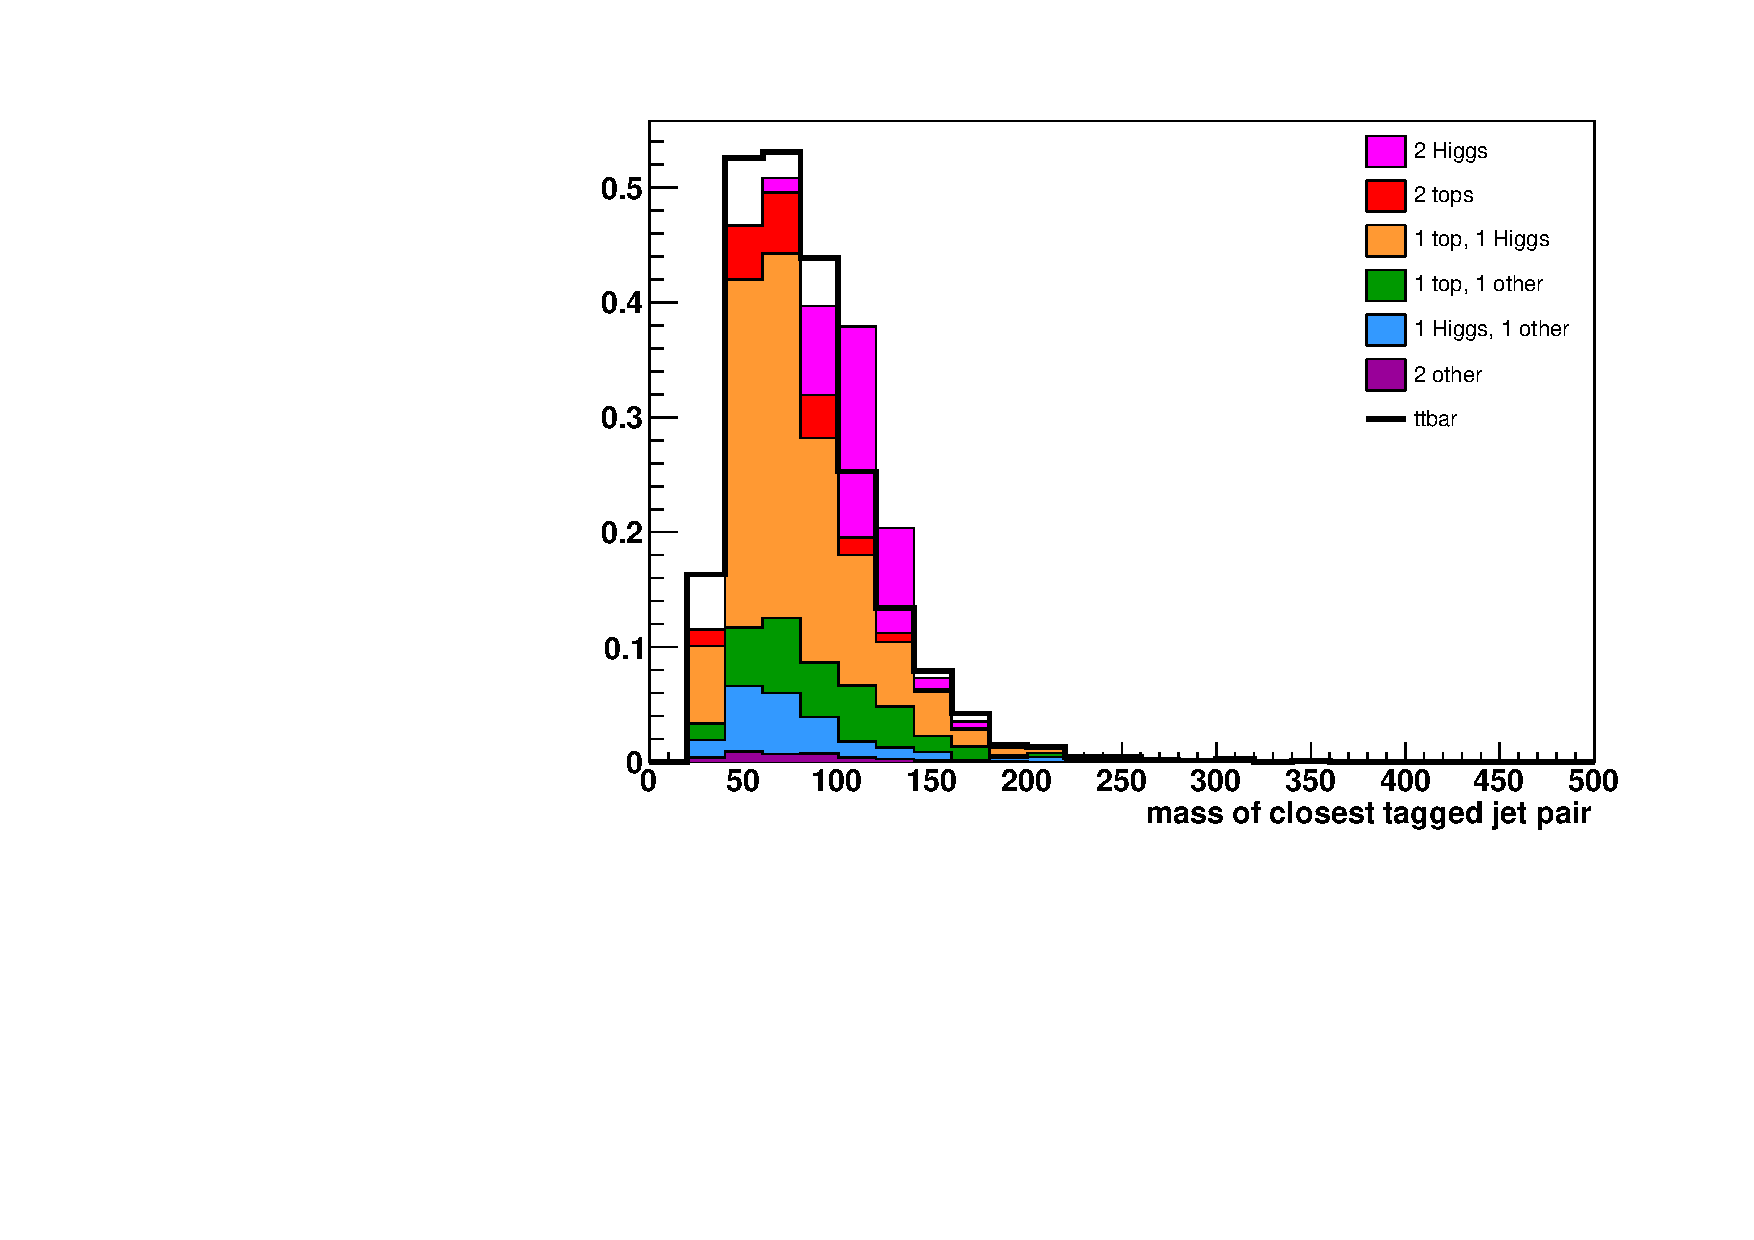
\includegraphics[width=0.7\textwidth]{Figures/Analysis_1_Diagrams/h_closestDR_mass_tag_tag_ge4t_rebin.pdf}
  \caption{This figure shows the breakdown of jet-to-parton
   assignments for the two jets with the minimum $\Delta R$
  separation in the event for events with greater or equal 4
  $b$-tagged jets.}\label{fig:tagMassCombinatorics}  
\end{figure}

\par The largest background contribution is $t\bar{t}+$jets
production.  This process can be decomposed in terms of the flavour of
the extra jets produced in the event.  For this analysis, the
inclusive $t\bar{t}$jets process is broken into three sub-proccesses:
$t\bar{t}+$ light flavor jets where one or more 
of the jets is mistagged, $t\bar{t}+c\bar{c}$ and $t\bar{t}+b\bar{b}$.
Smaller background contributions come from $W+$jets, $Z+$jets, single
top quark, diboson, and $t\bar{t}+W/Z$ production.  

\par In other Higgs searches involving the decay to two $b$-quarks,
the most powerful discriminating variable is the invariant mass of the
$b\bar{b}$ pair, which has a peak at the mass of the Higgs.  However, for
$t\bar{t}H$ production, with a final state of four $b$-quarks, the
combinatorics of selecting the quarks coming from the Higgs, instead
of the $t\bar{t}$ system, prevents the reconstruction of a clear
resonant peak, as shown in figure \ref{fig:tagMassCombinatorics}.
This results in an additional loss of mass resolution, or smearing,
on the $b\bar{b}$ invariant mass spectrum. 

\par Although there is poor resolution on the Higgs boson resonance in
the $b$-quark dijet mass spectrum, there are a number of kinematic
variables that can be used to discrminate betweenthe $t\bar{t}+$jets
background and the $t\bar{t}H$ signal.  For example, the recoil of
the Higgs off of the $t\bar{t}$ system, the decay products of the top
quarks from the $t\bar{t}H$ signal will have, on average, a slightly
larger component of momentum transverse to the beam-line.
Additionally, the lager number of authentic $b$-jets in $t\bar{t}H$
events can be exploited through the likelihood value returned by a
$b$-tagging algorithm for all of the jets in the event.  By
themselves, none of these variables provide a large degree of
discriminating power to separate the $t\bar{t}H$ signal from the
large, and kinematically similar background.  Therefore, the
discriminating power of several variables is combined using a
multivariate analysis technique (MVA), which is used to set upper
limits on $t\bar{t}H$ production in the data set. 

\par The following sections will describe the analysis that was
carried out on the first 5 \fbinv~of data collected by the CMS
detector.  This includes definitions of the simulatied samples used to
estimate the expected backgrounds in data, the event selection used to
isolate the $t\bar{t}H$ signal, the application of MVA techniques,
evaluation of systematic uncertainties, and upper limit setting on the
production rate of $t\bar{t}H$. 


\section{Data and Simulated Samples}
\label{data_and_mc_overview}

\par $pp$ collision data is collected by the CMS detector, as
described in previous chapters.  The signal and background signatures
are estimated using Monte Carlo simulation techniques.  The simulation
involves the combination of the most current theoretical and emperical
information about the interactions of the known particles.  The
simulation of an event is decomposed into a sequence of calculations and
each signal and background process is calculated seperately.
Information about Monte Carlo event simulation techniques is taken
from reference \cite{Agashe:2014kda}.  

\par The first stage of event simulation for a given signal or
background process is to calculate the probability that some set
initial state particles with a certain momentum will create a final
state of particles with a certain momentum.  For example, in the case of
the \ttH signal, this is the probability that two protons travelling
towards each other along the z-axis (beam-line), each with a given
energy and momentum, will produce a top quark pair and a Higgs boson,
each with some momentum vector, $\hat{p}_{t}$, $\hat{p}_{\bar{t}}$,
$\hat{p}_{H}$, which points into the hermetic CMS detector.  As
discused in section \ref{qft_overview}, this probability is calculated
by examing the lagrangian of the theory describing the process and
calculating its scattering amplitude, to some order in perturbation
theory, using the Feynman rules derived from the lagrangian.  The
scattering amplitude is a multi-dimensional probability function,
which depends on the inital and final state momentum of the particles
in the process.  Thus, given some intial state momentum, $p_{i}$, it tells you
the probability to produce a final state particle with mometum
$p_{f}$.  It is understandable that the scattering amplitude is
often reffered to as a matrix element, since given a vector of initial
state particles with a certain momentum, the scattering amplitude
would be a matrix, whose elements would give the probability of
creating the vector of final state particles.  

\par Since protons are composite objects, when they
collide, it is their quarks or gluons which are actually interacting.
The momentum distribution of each of the valence quarks, the gluons,
and the sea quarks, which account for quantum fluctuations that
temporarily create all other quark flavours inside the proton, is described by
a Parton Distribution Function (PDF).  The PDF describes what fraction
of the proton's momentum is distributed among each of its
constituents.  Due to the large strength of the QCD interactions that
bind the quarks together, the PDF cannot be calculated perturbitavely
from QCD.  It has been measured empircally, and is composition of the
results of several experiments over the past decades.  

\par Event generator algorithms are computer programs
that, given a lagrangian of particle theory, will calculate the
matrix element for a given process.  Then, the generator is provided
with values of the momentum of the intial state particles.  For
protons, this would the beam energy of the LHC.  To assign mometum
values to the constinuent quarks or gluons that actually participate
in the interaction, random values are sampled from the probability
distributions described by a PDF that is provided to the algorithm.
Given a choice of momentum for the input particles, a value and
direction of the momentum for each of the final state particles is
sampled from the probability function provided by the calculated the
matrix element (ME).  The process of randomly sampling a probability
function, in order to conduct a calculation, is known as a Monte Carlo
sampling technique.    

\par In the case where final state particles are quarks or gluons,
also known as partons, an additional calculation is necessary to
create the physical hadron states.  First, the decay sequence of each
parton is calculated until the decay products reach a user defined
value, known as the hadronization scale.  This decay sequence is
referred to as the parton shower (PS), since each parton creates a
multitude, or a shower, of additional partons.  Once the parton shower
is calculated, each of the colored partons are transformed into
color-singlet primary hadrons, which themselves decay, and form
secondary hadrons.  This process, known as hadronization, results in a
collimated spray of hadrons, each with a component of momentum along
the original parton's direction.  These hadrons are clustered together
and referred to as a hadron jet.   

\par Once the hadronization is completed, the next stage of the event
generation is to simulate the response of the CMS detector when this
process occurs at the interaction point where the LHC beams are made
to collide.  The Geant 4 detector simulation framework is used to
create a model of each and every detector element, electronic readout,
and mechanical support structures that make compose CMS.  Geant 4 is
also about to describe how energy is deposited into the different
types of material as a particle passes through each detector element,
simulating the response each element to presence of a particle in the
detector.  The digitization and signal acquisition of the electronics
that read-out the detector elements is also simulated.  

\par The final stage the generation of an event is the reconstruction
of the simulated detector signals into physics objects.  This process
is described in detail in the previous chapter.  It proceeds with
simulated, instead of real detector signals.  

\par The entire event simulation, reconstruction, and subsequent
anlaysis is implemented in a software framework that is known as CMS
Software (CMSSW).  

\subsection{Data Samples}
\label{data_overview}

\par The results presented here are based on the first 5.08\fbinv of the
2012 CMS dataset.  Data-sets are collected through HLT triggers and
stored offline for analysis.  Table~\ref{tab:dataSamples} lists the datasets used
for this analysis, which is composed of two runs of data collection
triggered on the presence of one muon or electron in an event.
The luminosities are quoted from a calculation performed with
minimum-bias events measured with the HF detector and have been
determined to have a 2.2\% uncertainty.   

\begin{table}[hbtp]\footnotesize
\centering
\begin{tabular}{|l|c|r|}
\hline\hline
 Dataset & Run Range & Integrated Luminosity \\
\hline
/SingleMu/Run2012A-PromptReco-v1/AOD & 190645--193621 & 0.87 fb$^{-1}$ \\
/SingleMu/Run2012B-PromptReco-v1/AOD & 193834--196531 & 4.21 fb$^{-1}$ \\
{\bf Total SingleMu} & {\bf 190645--196531} & {\bf 5.08 fb$\mathbf{^{-1}}$} \\
\hline
/SingleElectron/Run2012A-PromptReco-v1/AOD & 190645--193621 & 0.87 pb$^{-1}$ \\
/SingleElectron/Run2012B-PromptReco-v1/AOD & 193834--196531 & 4.21 pb$^{-1}$ \\
{\bf Total SingleElectron} & {\bf 190645--196531} & {\bf 5.08 fb$\mathbf{^{-1}}$} \\
\hline\hline
\end{tabular}
\caption{The datasets analyzed for this analysis.}
\label{tab:dataSamples}
\end{table}

\subsection{Signal Samples}
\label{signal_sample_overview}

\par The $t\bar{t}H$ signal is modeled using the Pythia Monte Carlo
generator.  Signal events were generated privately using the same
conditions and configuration as the "Summer'' MC campaign, which
generated the background samples used in this analysis and is a
central effort by a dedicated team of collaborators within the CMS
experiment.  The samples and associated cross sections used are listed in
Table~\ref{tab:sigSamples}.
 
\begin{table}[hbtp]\footnotesize
\centering
\begin{tabular}{|l|p{0.75\textwidth}|r|}
\hline\hline
Mass & Dataset & Cross Sect. \\
\hline
110 GeV/c$^2$ & /TTH\_HToAll\_M\_110\_8TeV\_FastSim\_pythia6/lannon-TTH\_HToAll\_M\_110\_8TeV \_FastSim\_pythia6-dff75535147f54d9d70123289019ff88/USER & 0.1887 pb \\
\hline
115 GeV/c$^2$ & /TTH\_HToAll\_M\_115\_8TeV\_FastSim\_pythia6/lannon\-TTH\_HToAll\_M\_115\_8TeV \_FastSim\_pythia6\-f8fb6149649333009ec8462da200312d/USER & 0.1663 pb \\
\hline
120 GeV/c$^2$ & /TTH\_HToAll\_M\_120\_8TeV\_FastSim\_pythia6/puigh\-TTH\_HToAll\_M\_120\_8TeV \_FastSim\_pythia6\-95111b4e2be5b1aa536a508d15d97f92/USER & 0.1470 pb \\
\hline
122.5 GeV/c$^2$ & /TTH\_HToAll\_M\_122p5\_8TeV\_FastSim\_pythia6/slaunwhj\-TTH\_HToAll\_M\_122p5\_8TeV \_FastSim\_pythia6\-1e2fdcc9a937df208692b27cb39e0444/USER & 0.1383 pb \\
\hline
125 GeV/c$^2$ & /TTH\_HToAll\_M\_125\_8TeV\_FastSim\_pythia6/lwming\-TTH\_HToAll\_M\_125\_8TeV \_FastSim\_pythia6\-191b19832235558f2b51f7486e9bfa14/USER & 0.1302 pb \\
\hline
127.5 GeV/c$^2$ & /TTH\_HToAll\_M\_127p5\_8TeV\_FastSim\_pythia6\_crabv2/jgwood\-TTH\_HToAll \_M\_127p5\_8TeV\_FastSim\_pythia6\_crabv2\-8cc2ab68d00e069563cff89a5be0e271/USER & 0.1227 pb \\
\hline
130 GeV/c$^2$ & /TTH\_HToAll\_M\_130\_8TeV\_FastSim\_pythia6/neu\-TTH\_HToAll\_M\_130\_8TeV \_FastSim\_pythia6\-5052c957a6363e9b1d5c2be444ffc86d/USER & 0.1157 pb \\
\hline
135 GeV/c$^2$ & /TTH\_HToAll\_M\_135\_8TeV\_FastSim\_pythia6/lwming\-TTH\_HToAll\_M\_135\_8TeV \_FastSim\_pythia6\-c8734ad98f674743d713309ea4b6ad34/USER & 0.1031 pb \\
\hline
140 GeV/c$^2$ & /TTH\_HToAll\_M\_140\_8TeV\_FastSim\_pythia6/lwming\-TTH\_HToAll\_M\_140\_8TeV \_FastSim\_pythia6\-cf0b11a8bdd755ec1ec3d7a35c9a88be/USER & 0.09207 pb \\
\hline\hline
\end{tabular}
\caption{List of signal MC datasets and cross sections used to determine the SM expectation.}
\label{tab:sigSamples}
\end{table}


\subsection{Background Samples}
\label{background_sample_overview}

\par In order to estimate the rate and kinematic behavior of the
backgrounds, this analysis primarily uses Monte Carlo (MC) samples
from the "Summer12'' MC campaign.  Most of the samples are
generated either with the Madgraph tree-level matrix element generator
matched to Pythia for the parton shower, or with the NLO
generator Powheg combined with Pythia.  These samples are
reconstructed with the same CMSSW version as the data samples listed
above.  Table~\ref{tab:bkgSamples} lists the
background MC samples and associated cross sections. 

\begin{table}[hbtp]\footnotesize
\centering
\begin{tabular}{|p{0.21\textwidth}|p{0.65\textwidth}|r|}
\hline\hline
Sample & Dataset & Cross Sect. \\
\hline
$t\bar{t}+$jets & /TTJets\_MassiveBinDECAY\_TuneZ2star\_8TeV\-madgraph\-tauola/Summer12\-PU\_S6\_START52\_V9\-v1/AODSIM & 225.197 pb \\
\hline
$t\bar{t}+W$ & /TTWJets\_8TeV\-madgraph/Summer12\-PU\_S7\_START52\_V9\-v1/AODSIM & 0.249 pb \\
\hline
$t\bar{t}+Z$ & /TTZJets\_8TeV\-madgraph\_v2/Summer12\-PU\_S7\_START52\_V9\-v1/AODSIM & 0.208 pb \\
\hline
$W+$jets & /WJetsToLNu\_TuneZ2Star\_8TeV\-madgraph\-tarball/Summer12\-PU\_S7\_START52\_V9\-v1/AODSIM & 36257.2 pb \\
\hline
$Z/\gamma^* +$~jets & & \\
$M\_{\ell\ell} > $50 GeV/c$^2$ & /DYJetsToLL\_M\-50\_TuneZ2Star\_8TeV\-madgraph\-tarball/Summer12\-PU\_S7\_START52\_V9\-v2/AODSIM & 3503.17 pb \\
10 GeV/c$^2 < M\_{\ell\ell} < $50 GeV/c$^2$ & /DYJetsToLL\_M\-10To50filter\_8TeV\-madgraph/Summer12\-PU\_S7\_START52\_V9\-v1/AODSIM & 860 pb \\
\hline
Single $t$ & & \\
$s$\-channel & /T\_s\-channel\_TuneZ2star\_8TeV\-powheg\-tauola/Summer12\-PU\_S7\_START52\_V9\-v1/AODSIM & 3.79 pb\\
$t$\-channel & /T\_t\-channel\_TuneZ2star\_8TeV\-powheg\-tauola/Summer12\-PU\_S7\_START52\_V9\-v1/AODSIM &  56.4 pb \\
$tW$ & /T\_tW\-channel\-DR\_TuneZ2star\_8TeV\-powheg\-tauola/Summer12\-PU\_S7\_START52\_V9\-v1/AODSIM & 11.1 pb \\
\hline
Single $\bar{t}$ & & \\
$s$\-channel & /Tbar\_s\-channel\_TuneZ2star\_8TeV\-powheg\-tauola/Summer12\-PU\_S7\_START52\_V9\-v1/AODSIM & 1.76 pb\\
$t$\-channel & /Tbar\_t\-channel\_TuneZ2star\_8TeV\-powheg\-tauola/Summer12\-PU\_S7\_START52\_V9\-v1/AODSIM & 30.7 pb \\
$tW$ & /Tbar\_tW\-channel\-DR\_TuneZ2star\_8TeV\-powheg\-tauola/Summer12\-PU\_S7\_START52\_V9\-v1/AODSIM  & 11.1 pb \\
\hline
$WW$ & /WW\_TuneZ2star\_8TeV\_pythia6\_tauola/Summer12\-PU\_S7\_START52\_V9\-v1/AODSIM & 54.8 pb \\
\hline
$WZ$ & /WZ\_TuneZ2star\_8TeV\_pythia6\_tauola/Summer12\-PU\_S7\_START52\_V9\-v1/AODSIM & 32.3 pb \\
\hline
$ZZ$ & /ZZ\_TuneZ2star\_8TeV\_pythia6\_tauola/Summer12\-PU\_S7\_START52\_V9\-v1/AODSIM & 7.7 pb \\
\hline\hline
\end{tabular}
\caption{List of background MC datasets and cross sections used for normalization.}
\label{tab:bkgSamples}
\end{table}

\subsection{MC pileup reweighting}
\label{mc_pileup_reweight_overview}

\par During 2012 data collection, the LHC provided increasingly
large instantaneous luminosities to the CMS experiment.  Consequently,
the average number of overlapping events reconstructed in single
detector readout window has also increased.  When these overlapping
events, known as pileup events, occur within the same bunch crossing,
which as reffered to as "in-time'' pileout.  Alternatively,
"out-of-time'' pileup, comes from energy deposits in the detector from
previous bunch crossings and from very early arrivals of particles
from the forthcoming bunch crossing.  Pileup events can affect many
aspects of the reconstruction a more interesting event, such as the
degradation of lepton isolation and jet energy resolution.  The
simulated samples used in the analysis must also have the same
distribution of pilup events as what was measured in the data.

\par During the generation of the simulated samples used in the
analysis, the average amount of expected pileup was unknown.  Events
were thus simulated with a conservatively large estimate of the pileup
distribution, so that if the measured data revealed a smaller average
value, the simulation could be reweighted to match the data.  
For the simulation, number of interactions is a user defined value
added to every generated event.  For the data, the number of pileup
interactions for each unit of time depends on the instantaneous luminosity for each bunch pair and the
total inelastic cross section, $\sigma_{inelastic}$, of the proton.
The value of $\sigma_{inelastic} = 69.4$ mb was found to describe the data
well.  To estimate the effect of the systematic uncertainty of this
choice, the value was varied by $\pm 7\%$.  

\par To guage the accuracy of the calibration of the pileup
distribution used in the simulated samples, a comparison of the
number of reconstruced vertices between data and the simulated
$t\bar{t}$ MC sample is shown in figure~\ref{fig:PUrewgt}.  The
unweighted MC distribution is shown in blue, the reweighted
distribution in red, and the measured data in black points.  After
reweighting, there is a good level of agreement between the data and
MC distributions.  

\begin{figure}[hbtp]
 \begin{center}
   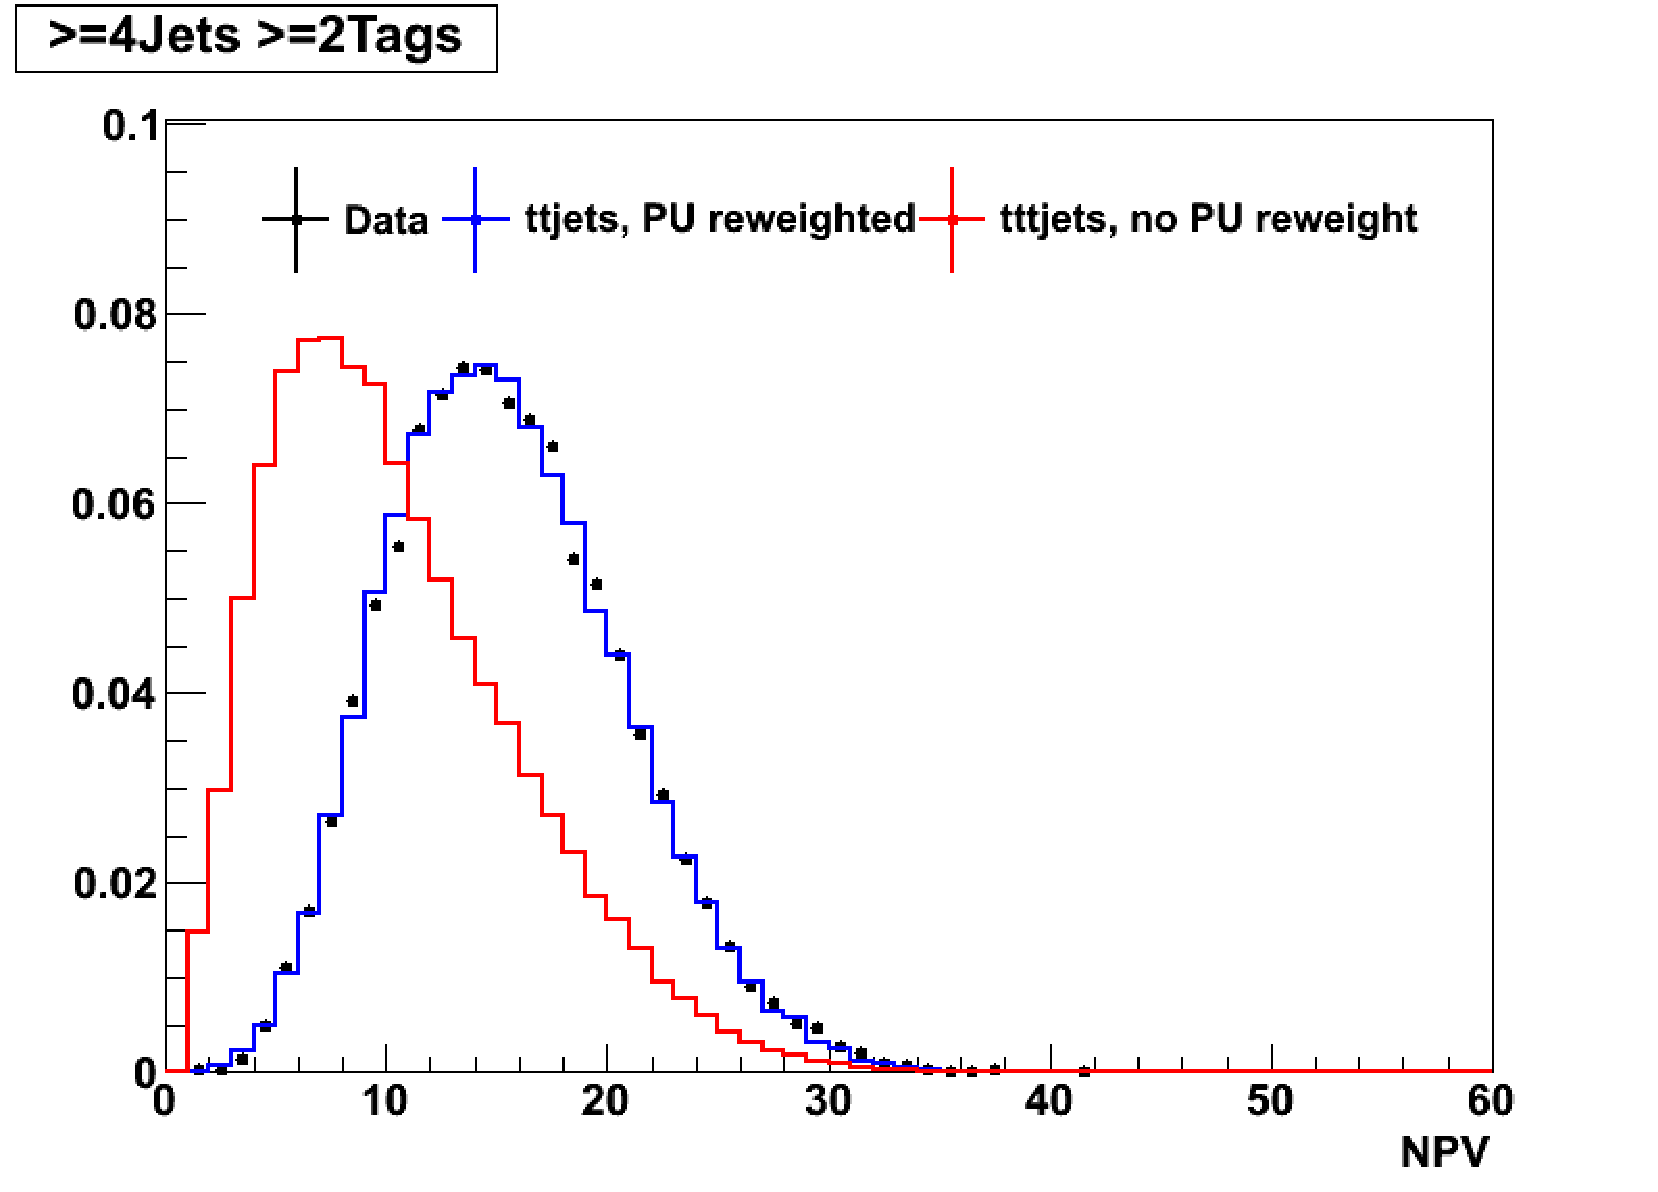
\includegraphics[width=0.5\textwidth]{Figures/Analysis_1_Diagrams/pileUpReWeighting_4Jincl2Tincl.pdf}
   \caption{Comparison of number of reconstructed vertices for data
     (black) and the $t\bar{t}$ MC sample before (blue) and after
     (red) pileup reweighting.  After pileup reweighting, the MC
     matches the data well.} \label{fig:PUrewgt}
 \end{center}
\end{figure}


\subsection{Additional Pileup Corrections}
\label{additional_pileup_reweight_overview}

\par Studies comparing the Monte Carlo simulations to observed
data revealed that the jet $p_T$ spectra was not well modeled.  Many
sources of this discrepancy were investigated, but the clearest
correlations arises when the 8 TeV data events are divided into three
categories according to their amount of pileup:

\begin{itemize}
\item Low PU, number of primary vertices $\leq$ 10
\item Medium PU, number of primary vertices from 11 to 15
\item High PU, number of primary vertices $\geq$ 16
\end{itemize}

\noindent  The modeling of jet $p_{T}$ was worse for events with a
larger number of pileup events overlapping in the detector. The same
effect was present for the majority of the jets in the event,
evidenced by the discrepancy in the $H_{T}$ distribution, shown in
figure \ref{fig:HTreweight}, where $H_{T}$ is defined as the scalar
sum of the transverse momentum for reconstructed jets in the event:

\begin{equation}
H_{T} = \sum_{i}^{jets} p_{T}^{i}
\end{equation}

\noindent The effect makes the data have a softer $p_{T}$ spectrum
than the simulations.  The same effect was observed in 7 TeV data
as well.  It was present, even after employing several sophisticated
reconstruction techniques designed to mitigate pileup effects.  These
techniques included the removal of charged hadrons in the
particle-flow algorith, not associated with the primary vertex and
re-weighting the simulated samples to match the pileup distribution
measured in the data.  

\begin{figure}[hbtp]
 \begin{center}
   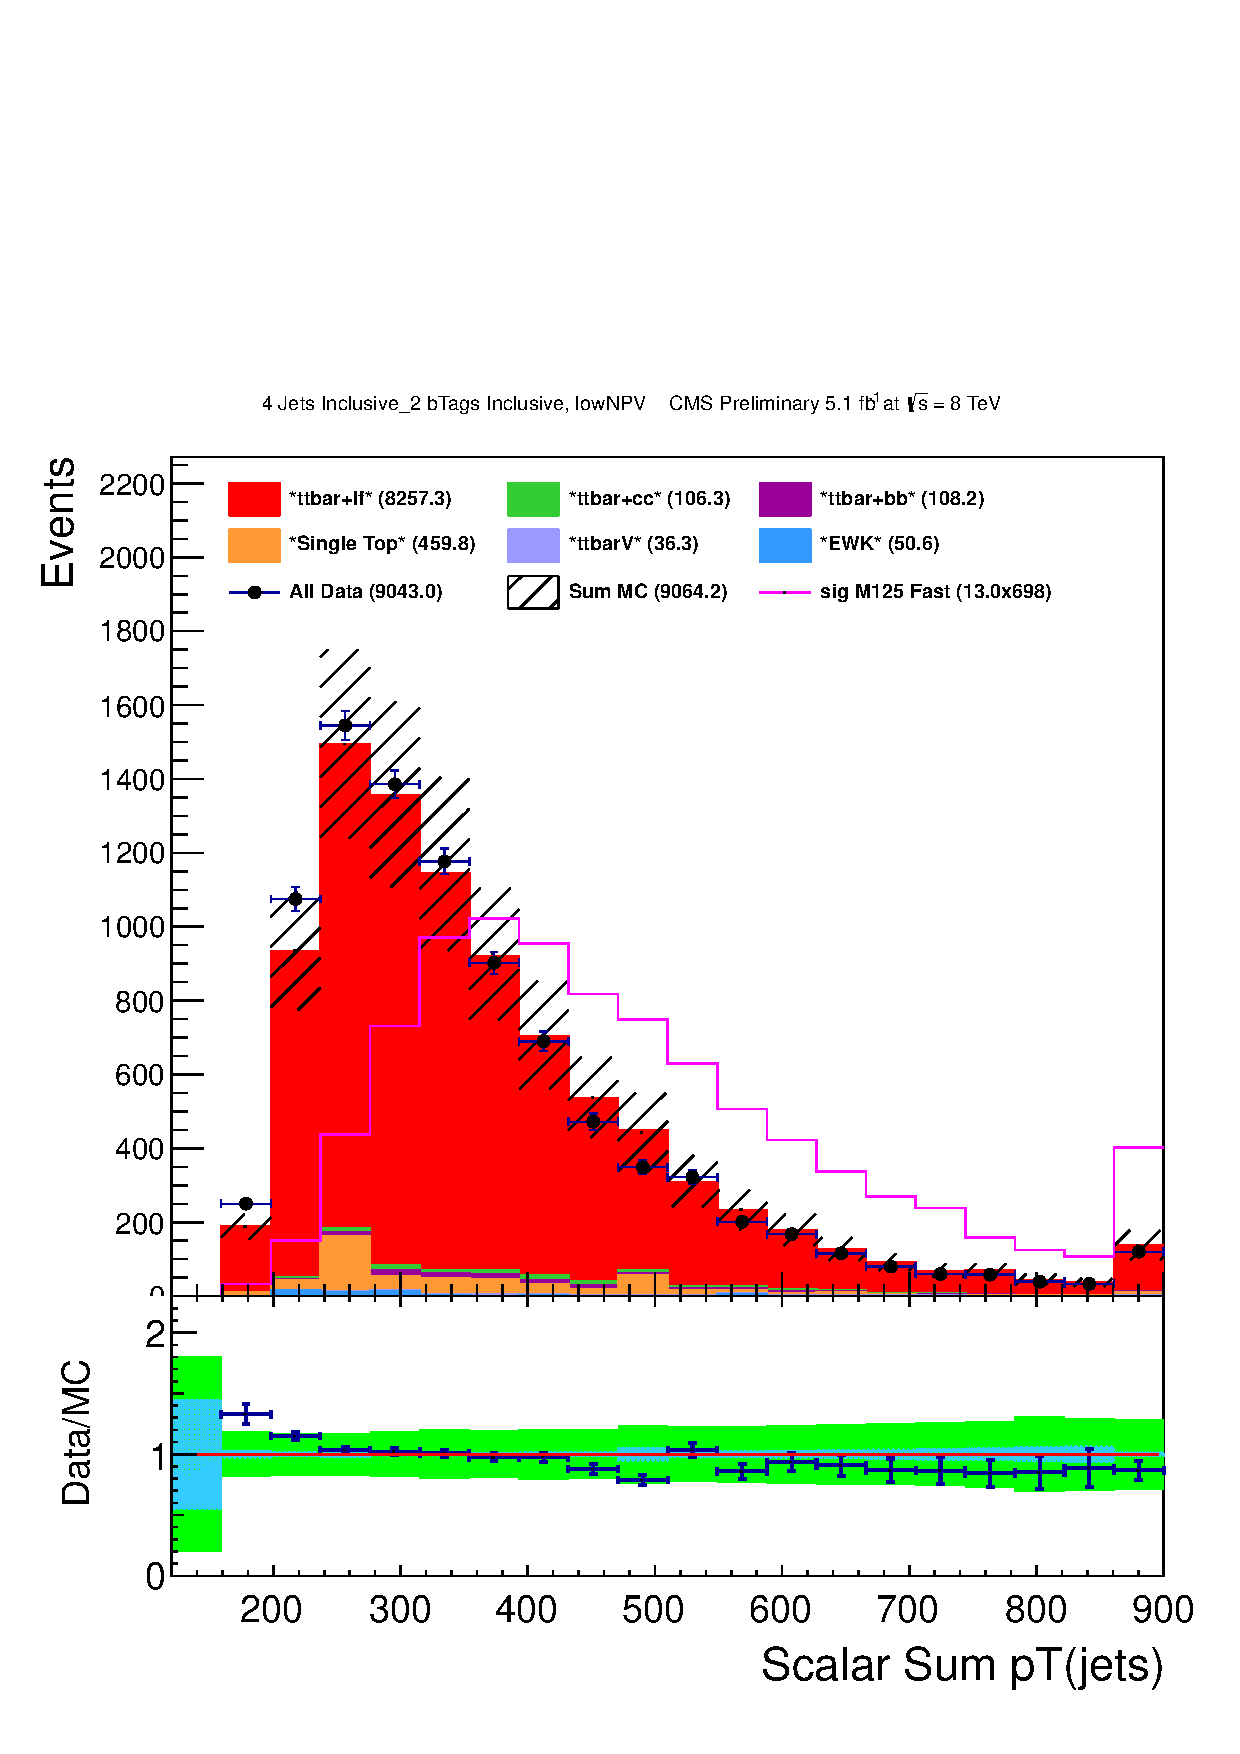
\includegraphics[width=0.30\textwidth]{Figures/Analysis_1_Diagrams/d2MCPlots_Ht_cut10_4J_2T_lowNPV_Combined.pdf}
   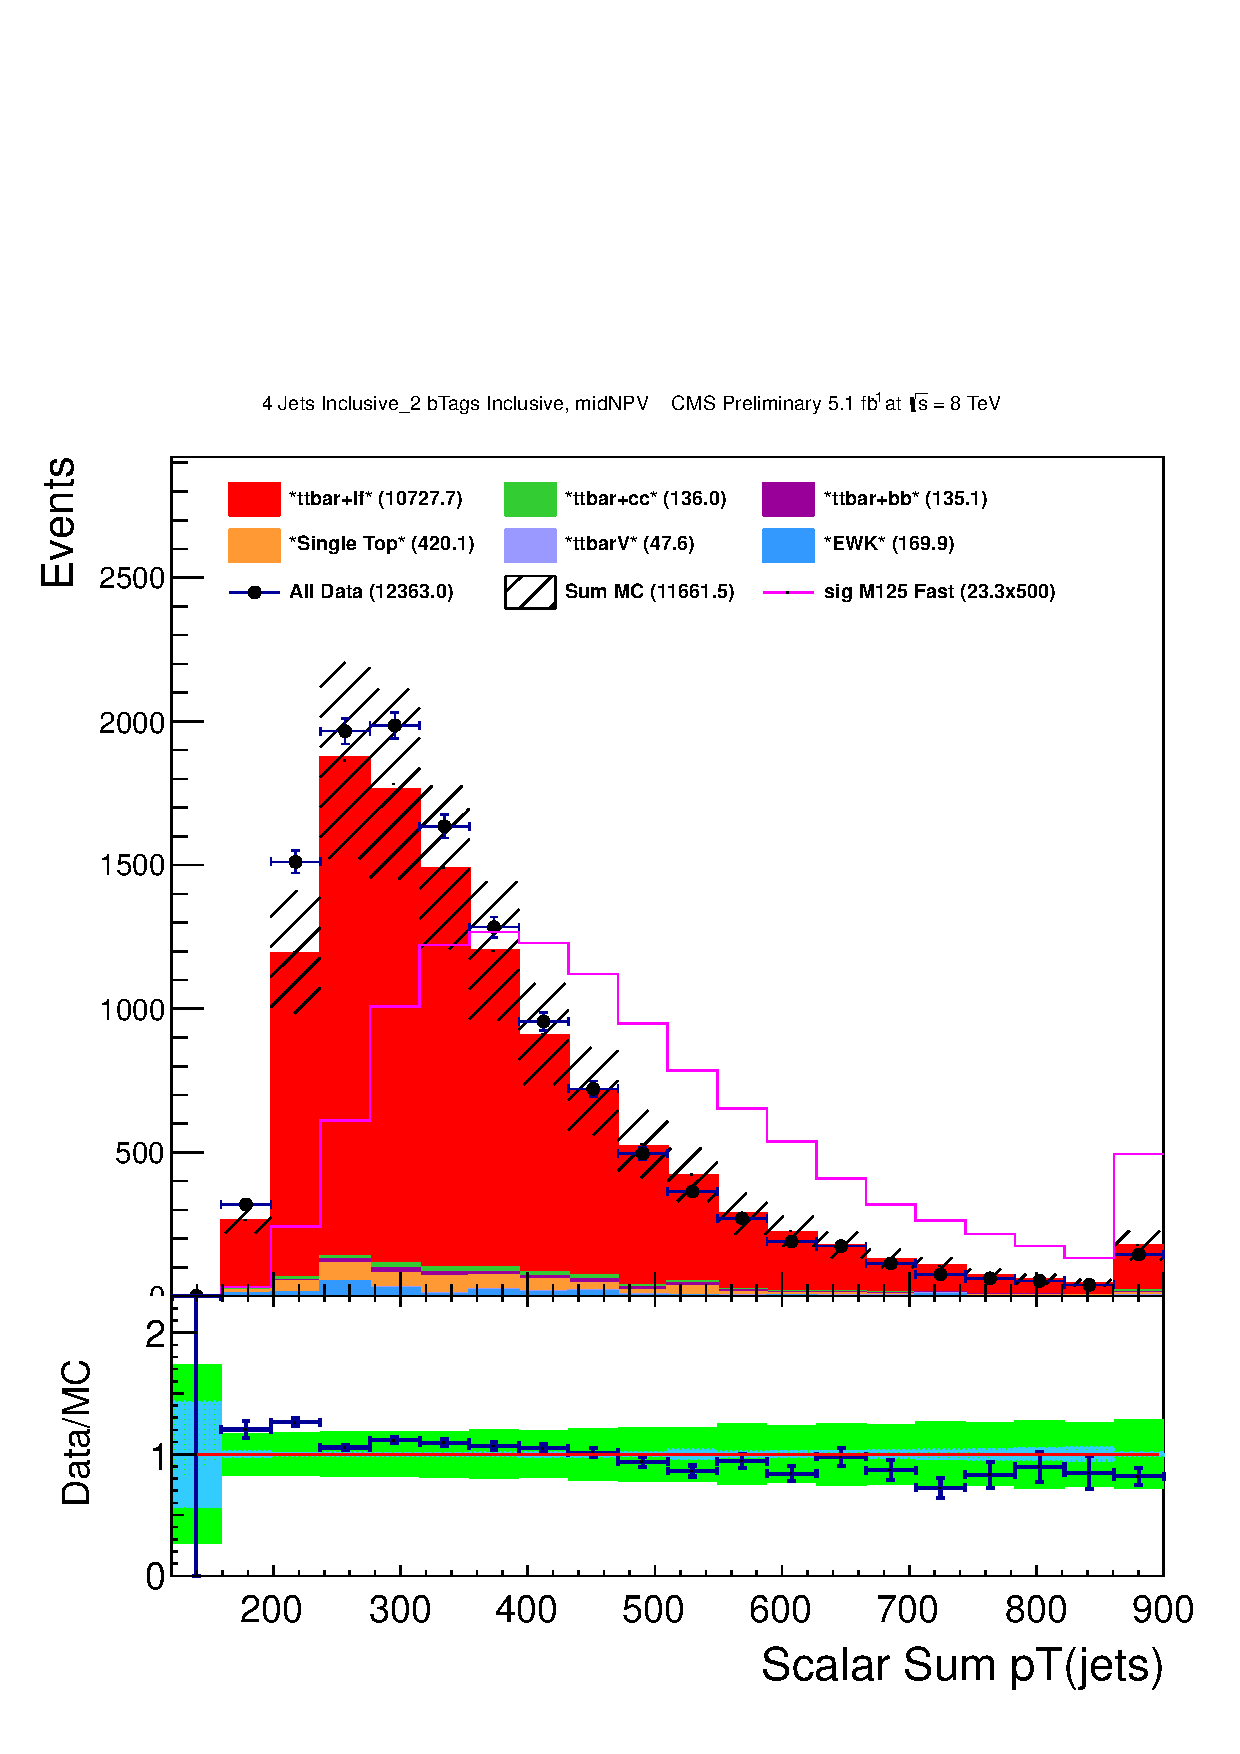
\includegraphics[width=0.30\textwidth]{Figures/Analysis_1_Diagrams/d2MCPlots_Ht_cut11_4J_2T_midNPV_Combined.pdf}
   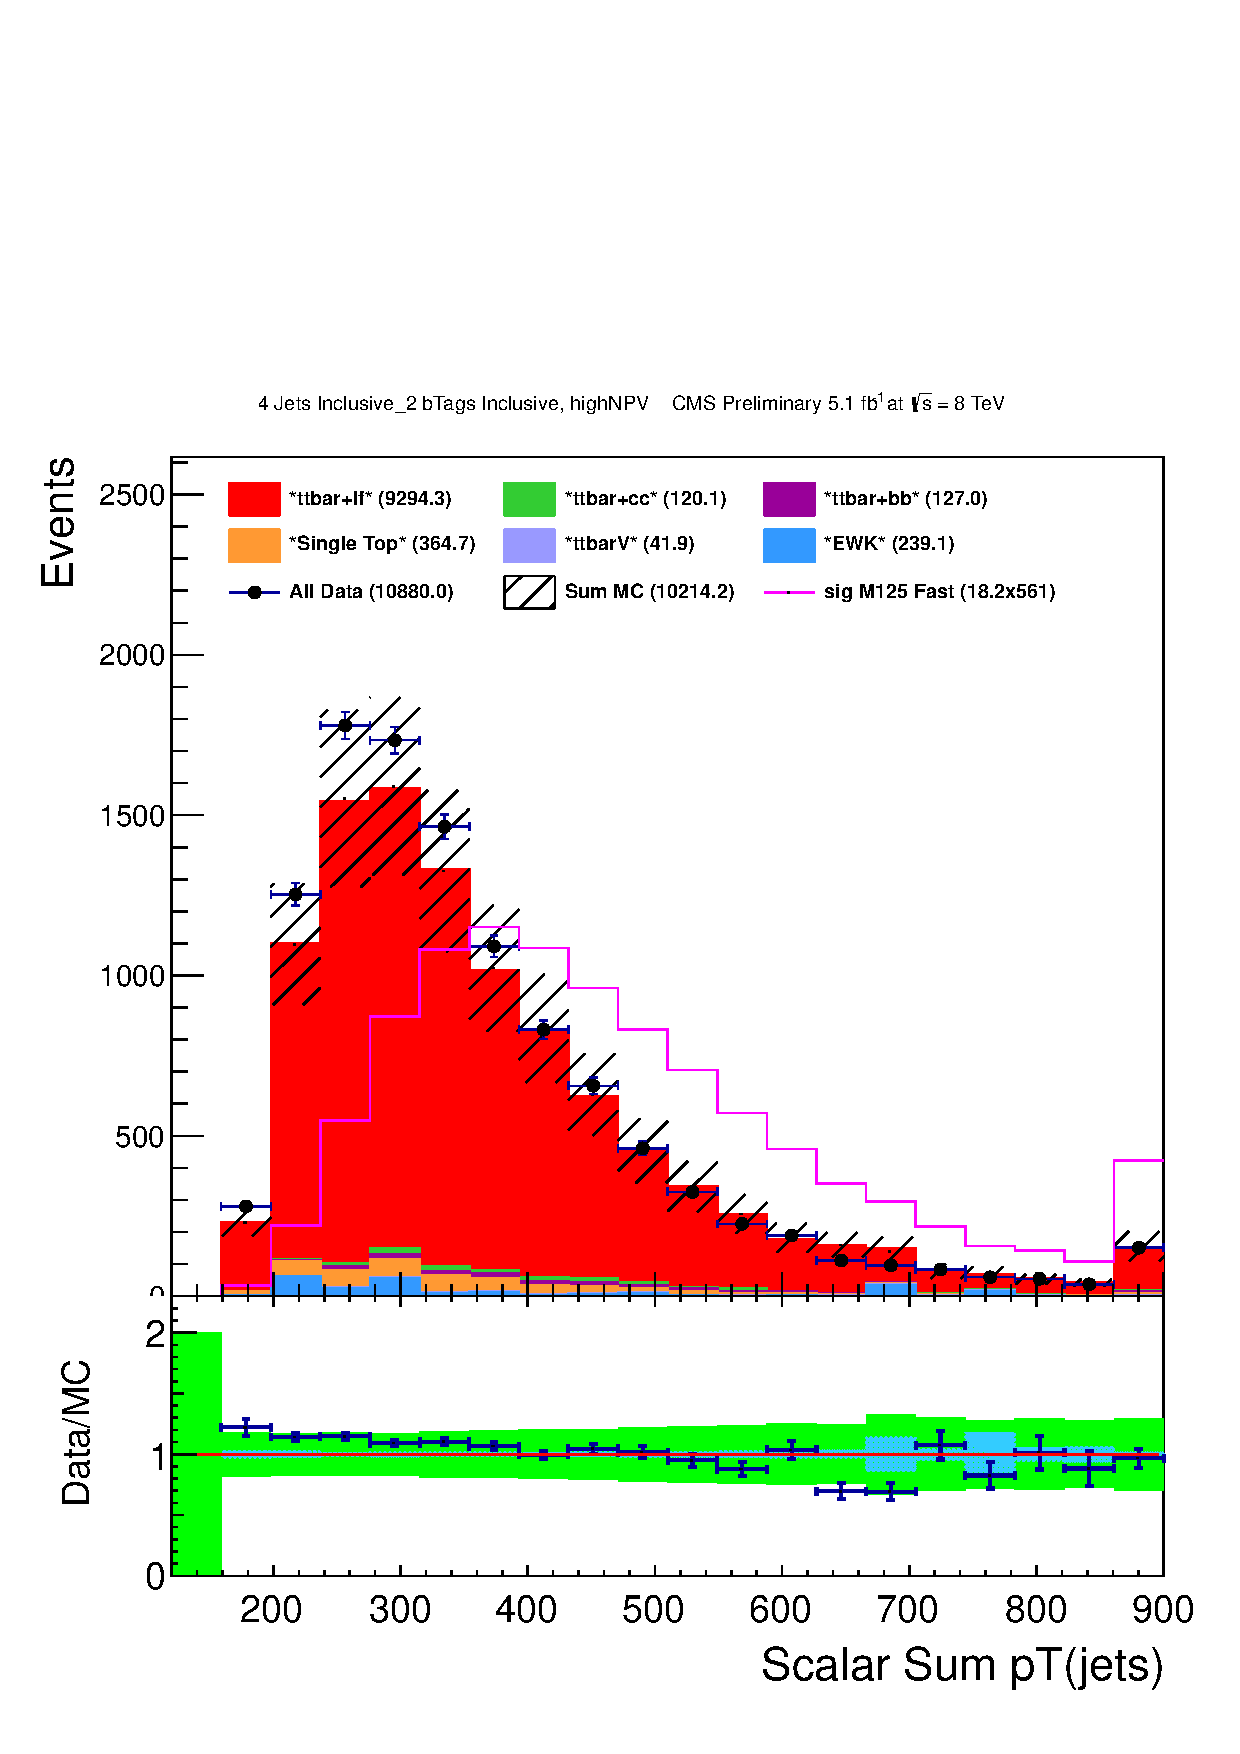
\includegraphics[width=0.30\textwidth]{Figures/Analysis_1_Diagrams/d2MCPlots_Ht_cut12_4J_2T_highNPV_Combined.pdf}
   \caption{$H_{T}$ distribution for 8 TeV lepton plus jet events with $\geq 4 jets$ and $\geq 2 tags$ shown
   for different amounts of pileup. The left-hand plot shows low pileup, the middle plot shows
   medium pileup, and the right-hand plot shows high pileup.}
   \label{fig:HTreweight}
 \end{center}
\end{figure}



\par Although the exact underlying cause of the jet mis-modeling
effect was not able to be identified, the magnitude of the effect
seemed to be related to the number of pileup events.  As such, an
additional correction factor is needed to account for the remaining
difference in pileup effects between data and Monte Carlo.  The 
correction factor was calculated from data that was dominated by
background events, with a single lepton, $\geq 4$ jets, and
$\geq 2$ tags. The expected signal-to-background ratio in this sample
is 0.002, which is low enough that the correction factor will not be
biased by signal events.  The correction factor is based on the $H_{T}$
distribution for data and Monte Carlo for Low pileup (PU), Medium PU,
and High PU events. The correction factor is the bin-by-bin ratio of
the data and the Monte Carlo $H_{T}$ distributions in each PU
category.  By preparing a separate correction factor for each PU
category smaller adjustments were made to well-modeled Low PU events and
larger adjustments to the poorly modeled High PU events.  $H_{T}$
shows the same mis-modelling as each of the jet $p_{T}$s and it
effects all of the jet $p_{T}$s. This makes it a natural choice for a
correction factor.

\par In order to evaluate the systematic shape uncertainty introduced
by the correction factor, the uncorrected simulated distributions are
used as $-1\sigma$ systematic uncertainty and the $+1\sigma$
uncertainty is determined by doubling the correction factor. The
factor of two for the $+1\sigma$ variation is motivated by the deisre
to provide a large enough systematic uncertainty to cover any possible
over-correction of the simulations.  This is a reasonable choice
because it creates a deviation that is the same size as the original
observed difference between data and simulations. 

\par The correction factor and uncertainty improved the agreement
between data and Monte Carlo. Figure \ref{fig:HTBeforeAfter}
compares the $H_{T}$ distributions before and after
reweighting. The data-to-MC ratio plots are the clearest indicators of
the improvement from the correction factor. Before the correction,
the $H_{T}$ ratio plot forms a line with a slope. After the correction
the slope is gone.

\begin{figure}[hbtp]
 \begin{center}
   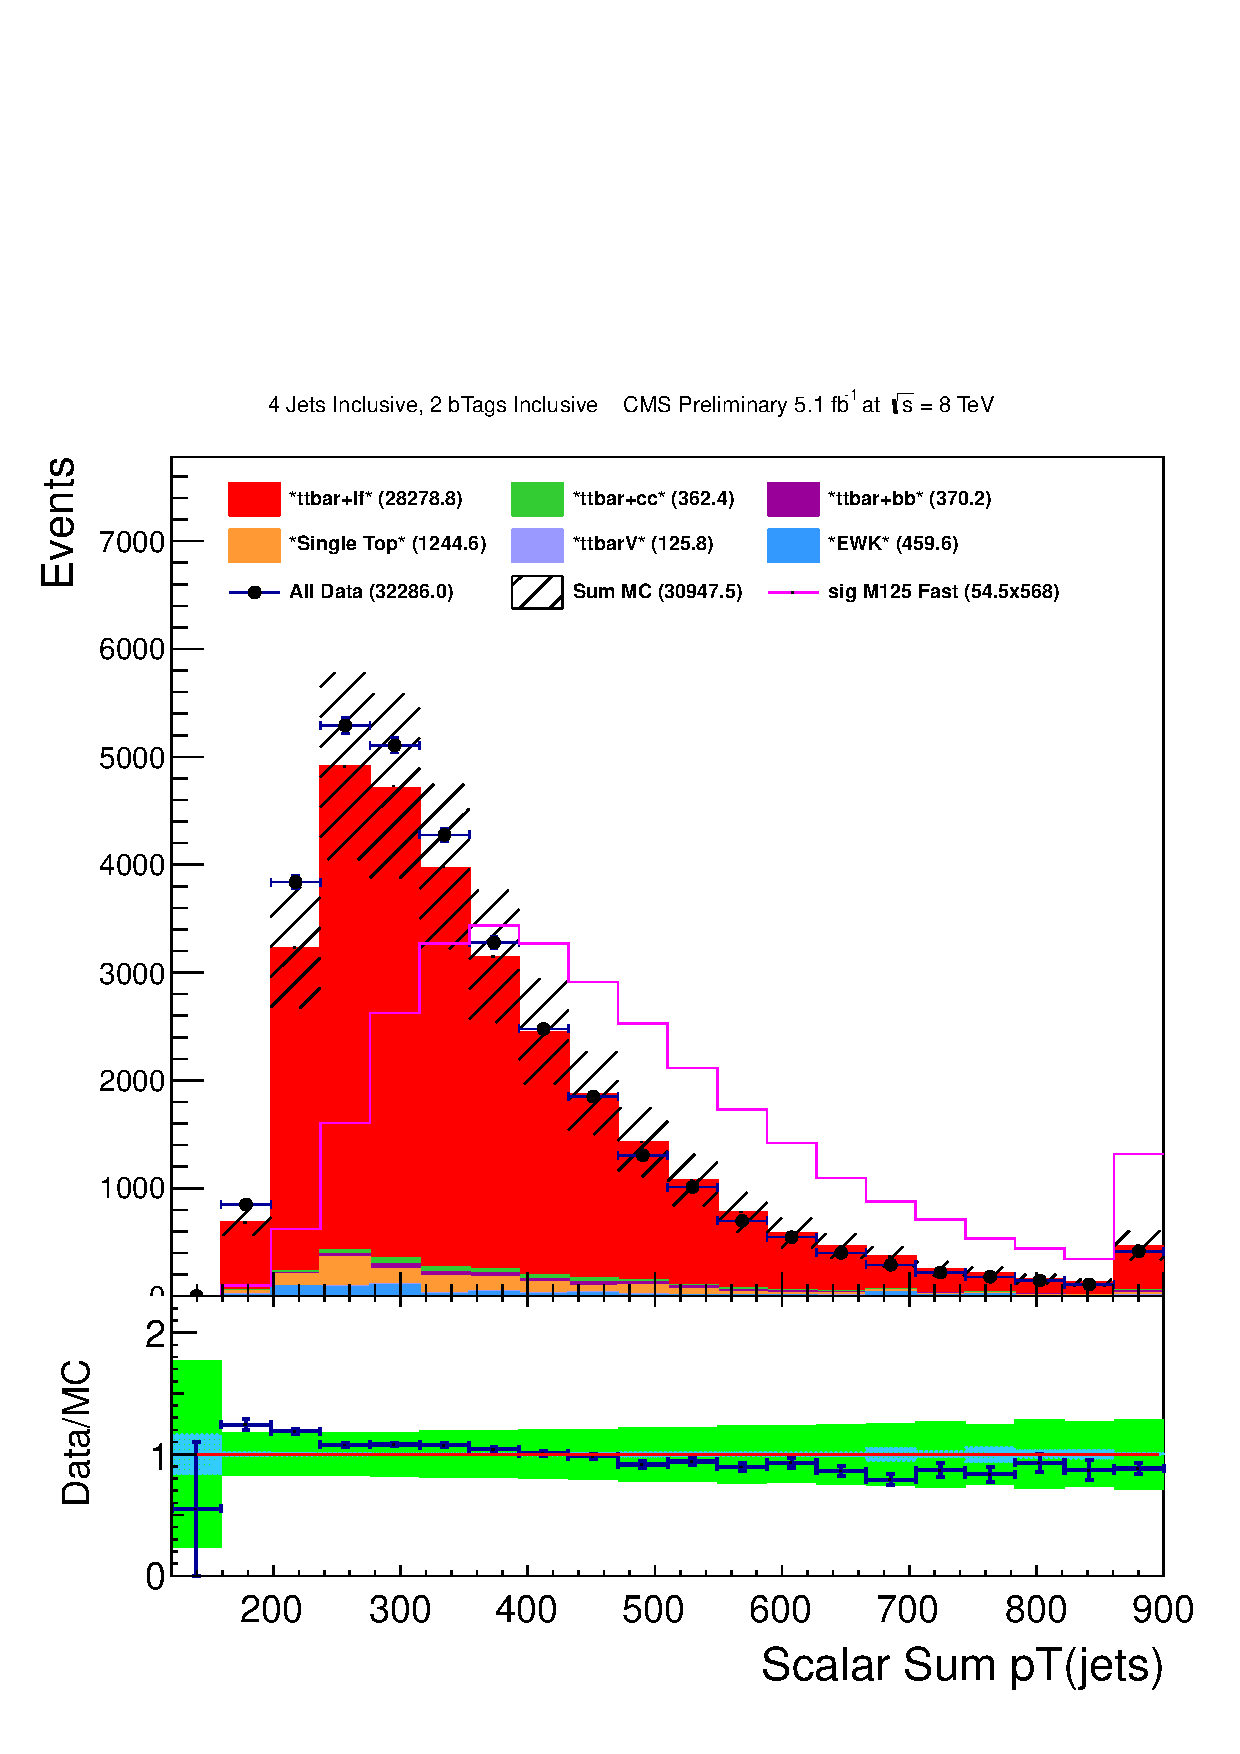
\includegraphics[width=0.45\textwidth]{Figures/Analysis_1_Diagrams/d2MCPlots_Ht_cut0_4JIncl_2TIncl_Combined.pdf}
   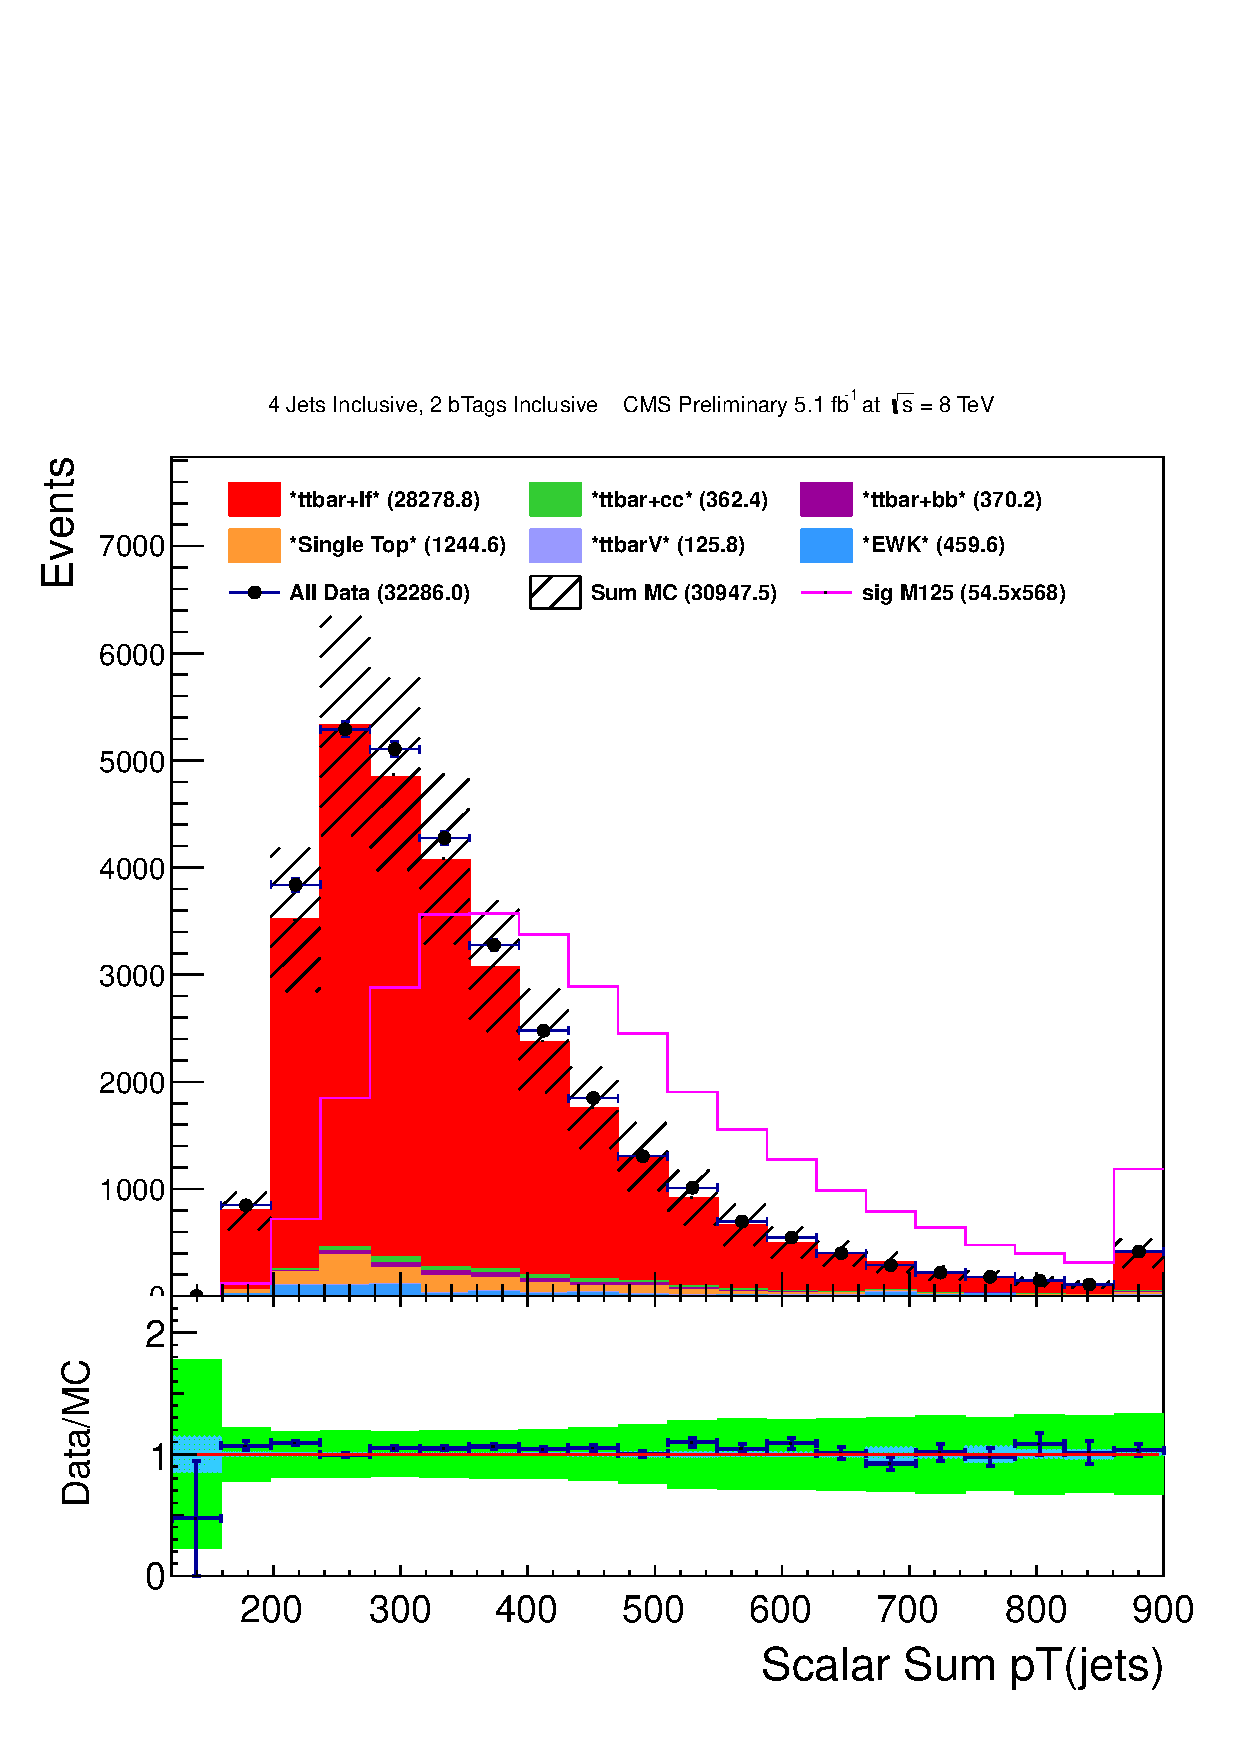
\includegraphics[width=0.45\textwidth]{Figures/Analysis_1_Diagrams/d2MCPlots_Ht_cut0_4JIncl_2TIncl_Combined_HtWgt.pdf}
   \caption{$H_{T}$ distribution for 8 TeV lepton plus jet events with
   $\geq 4 jets$ and $\geq 2 tags$. The left-hand plot shows the
   distribution before correction. The right-hand plot shows the
   distribution after correction. Note that the ratio in the right-hand
   plot is flatter than the left-hand plot.}
   \label{fig:HTBeforeAfter}
   \end{center}
\end{figure}




\section{Event Selection}
\label{event_selection_overview}

\par This section defines the common physics objects and event
selection requirements.  Leptons are classified into two categories,
tight and loose, defined for muons in section
\ref{muon_selection_overview} and for electrons in
\ref{electron_selection_overview}.  For this analysis, exactly one
tight muon or exactly one tight electron is required and events with
any additional loose leptons are rejected. 


\subsection{Event cleaning}
\label{event_cleaning_overview}

\par For data and MC events, certain cuts are applied to remove events
that are either non-physical or that come from non-collision events,
such as instrumental noise or beam backgrounds.  In the data, every
event is required to pass the following filters:

\begin{itemize}
  \item CSC tight beam halo filter - Secondary particles are produced
    in showers which are initiated by collisions of the beam with
    residual gas inside the LHC vacuum chamber or by interactions of
    the particles with a large transverse emmitance with limiting
    apertures.   
  \item HBHE noise filter with isolated noise rejection - this filters
    spurious signals from the HCAL barrel and endcap subdetectors which
    are not associated with particles measured in a collision event. 
  \item HCAL laser filter - ensures that data is not taken
    simulatenous with the laser calibration system
  \item ECAL dead cell trigger primitive (TP) filter - removes dead
    or noisy ECAL cells from being used in the reconstruction, these
    compose $<1\%$ of the total crystals in the ECAL
  \item Tracking failure - designed to catch events with too few tracks
  \item Noisy SCs in EE - new filter from the ECAL Detector
    Performance Group (PDG), and validated by the MET Physics Object
    Group (POG)
\end{itemize}

\noindent which are described in ~\cite{METfilters}.

\par Additionally, beam scraping events are filtered based on the fraction
of good tracks.  We require that at least 25\% of tracks are of high
purity.  Finally, every data event must contain at least one primary
vertex (PV) that passes the following selection:

\begin{itemize}
  \item The number of degrees of freedom used to find the PV must be larger than 4,
  \item The absolute value of the \(z\)-coordinate of the PV must be smaller than 24 cm,
  \item The absolute value of the \(\rho\)-coordinate of the PV must
    be smaller than 2 cm,
  \item The PV must not be identified as fake.
\end{itemize}

\subsection{Trigger}
\label{trigger_overview}

\par Each data and MC event is required to pass passes one of the
triggers in Table~\ref{tab:LepJetTriggerTable}, which are a subset of the
total number of SingleMu and SingleEle HLT triggers available.  
Muon+jet events must pass the SingleMu trigger, while
electron+jet events must pass the SingleEle trigger.  

\begin{table}[hbtp]\footnotesize
\centering
\begin{tabular}{|c|l|}
\hline\hline
Dataset & Trigger Name \\
\hline
SingleMu & HLT\_IsoMu24\_eta2p1\_v* \\
\hline
SingleEle & HLT\_Ele27\_WP80\_v* \\
\hline\hline
\end{tabular}
\caption{List of lepton+jets triggers}
\label{tab:LepJetTriggerTable}
\end{table}


\subsection{Muon Selection}
\label{muon_selection_overview}

\par In this analysis, muons are selected from the set of
"particle-flow' muon'' objects that have been reconstructed in the
event.  Muons are classified into two categories: tight and loose,
according to the quality of their reconstruction.  This is ensured by
applying the selection cuts shown in
Table~\ref{tab:TightLooseMuTable}.  The cuts are defined as follows:

\begin{itemize}
  \item $p_{T}$ - the component of the momentum transverse to the
    beam-line.
  \item PFRelIso - this is the quantity known as relative isolation,
     computed by the particle flow algorithm.  It is a ratio of the
     energy deposits remaining in the calorimeter and tracker, after
     the contribution from the muon has been removed, in a cone size
     $\Delta$R = 0.3, around the muon track.
  \item $|\eta|$ - the absolute value of the psuedorapdity of the muon
  \item ID - This refers to whether the muon was reconstructed with a
    $\chi^{2}$ fit to the tracks from the tracker only (tracker muon),
    the tracker and the muon chambers (global muon), or if the
    particle was reconstructed from the particle-flow algorithm
    (PFmuon)
  \item $N_{layers}($tracker$)$ - the number of layers in the tracker
    with hits used in the muon track reconstruction
  \item ${X}^{2}$ of track fit - the reduced $\chi^{2}$ (raw
    $\chi^{2}$/Number of Degrees of Freedom in the fit), typically a
    value of 1 indicates the fit is describes the data well 
  \item $N_{layers}($pixel$)$ - the number of layers in the inner
    pixel detector with hits used in the muon track reconstruction
  \item $N_{segments}(\mu)$ - the number of segments in the muon
    chambers used to the reconstruct the muon tracks
  \item $|d0($BS$)|$ - the absolute value of the transverse distance
    of the extrapolated muon track to the primary vertex, as
    calculated from the beam spot (BS)
  \item $|dZ($BS$)|$ - the absolute value of the longitudinal distance
    of the extrapolated muon track to the primary vertex
\end{itemize}

\begin{table}[hbtp]\footnotesize
\centering
\begin{tabular}{|l|c|c|}
\hline\hline
Cuts & Tight $\mu$ & Loose $\mu$ \\
\hline
$p_{T}$ & \textgreater 30 GeV/c & \textgreater 10 GeV/c \\
\hline
PFRelIso$(0.4)$ & 0.12  & \textless 0.2 \\
\hline
$|\eta|$ & \textless 2.1 & \textless 2.5 \\
\hline
ID & Global Muon & Global Muon or Tracker Muon \\
\hline
ID & PFMuon & PFmuon \\
\hline
$N_{layers}($tracker$)$ & \textgreater 5 & \\
\hline
${X}^2$ of track fit & \textless 10 & \\
\hline
$N_{layers}($pixel$)$ & \textgreater 0 & \\
\hline
$N_{segments}(\mu)$ & \textgreater 1 & \\
\hline
$|d0($BS$)|$ & \textless 0.2 cm & \\
\hline
$|dZ($BS$)|$ & \textless 0.5 cm & \\
\hline\hline
\end{tabular}
\caption{Tight and loose muon definition}
\label{tab:TightLooseMuTable}
\end{table}



\subsection{Electron Selection}
\label{electron_selection_overview}

\par Electrons are selected from the set of "particle-flow electron''
objects reconstructed in the event.  Similarly to muons, electrons are
classified into two categories: tight and loose, according to the
quality of their reconstruction.  The selection cuts are shown in the
Table ~\ref{tab:TightLooseEleTable}.  The definitions are identical to
the ones provided in section \ref{muon_selection_overview}.
Additional variables not described are:

\begin{itemize}
  \item $E_{T}$ - the transverse energy of the electron, which due to
    its relatvily light mass, is approximately equal to its $p_{T}$
  \item ID - electron ID is passed on a multivariate analysis (MVA)
  technique, which provides a discriminant value to seperate fake from
  real electrons, and is trained with events that are required to pass
  a HLT trigger (mvaTrigV0), or not (mvaNonTrigV0).  The
  "passConversionVeto'' ID ensures that the electron has not been
  reconstructed from a photon which has converted to an electron
  positron pair
\end{itemize}

\begin{table}[hbtp]\footnotesize
\centering
\begin{tabular}{|l|c|c|}
\hline\hline
Cuts & Tight \emph{e} & Loose \emph{e} \\
\hline
$E_{T}$ & \textgreater 30 GeV/c$^2$ & \textgreater 15 GeV/c$^2$ \\
\hline
PFRelIso$(0.3)$ & \textless 0.1 & \textless 0.2 \\
\hline
$|\eta|$ & \textless 2.5 & \textless 2.5 \\
\hline
ID & MVA ID("mvaTrigV0'') \textgreater 0.0 &  MVA ID("mvaNonTrigV0'') \textgreater 0.0\\
\hline
ID & passConversionVeto & passConversionVeto \\
\hline
$|d0(BS)|$ & \textless 0.02 cm & \\
\hline
$|dZ(PV)|$ & \textless 1 cm & \\
\hline\hline
\end{tabular}
\caption{Tight and loose muon definition}
\label{tab:TightLooseEleTable}
\end{table}


\subsection{Lepton selection and trigger efficiencies}
\label{trigger_efficiency_overview}

\par The cumulative reconstruction efficiency of id+isolation+trigger
has been calculated from data, as a function of pT and eta, as
shown in figure ~\ref{fig:effSFHLT} for electrons and muons.  In order
to reproduce the same the same response in the simulations as found in
data, an event-by-event scale factor is applied to correct for this
difference in effiency.  

\par The effiency in data was measured by selected events with two
tight muons, or two tight electrons with an invariant mass in a range
between 70 and 130 GeV.  This is centered on the $Z$ boson resonance,
and ensures that the selected leptons are authentic.  The two leptons
are additionally required to have opposite charge, which is measured
by the direction of the curvature of their tracks in the magnetic
field.  A "tag'' lepton is selected if has $p_{T}$>30 GeV, and passes
the appropriate muon or electron trigger.  The second lepton, the
"probe'' lepton, since selected as a pair coming from a $Z$ boson,
should be identical to the tag lepton, and thus should be identically
reconstructed.  The effiency is then the ratio of the number events where both
tag and probe leptons pass the $p_{T}$ and trigger requirements over
the number of events where only the tag lepton passes the $p_{T}$ and
trigger requirements.  This study is repeated in bins of $p_{T}$ and
$\eta$ to remove any kinematic dependence on lepton efficiency.  

\begin{figure}[hbtp]
 \begin{center}
   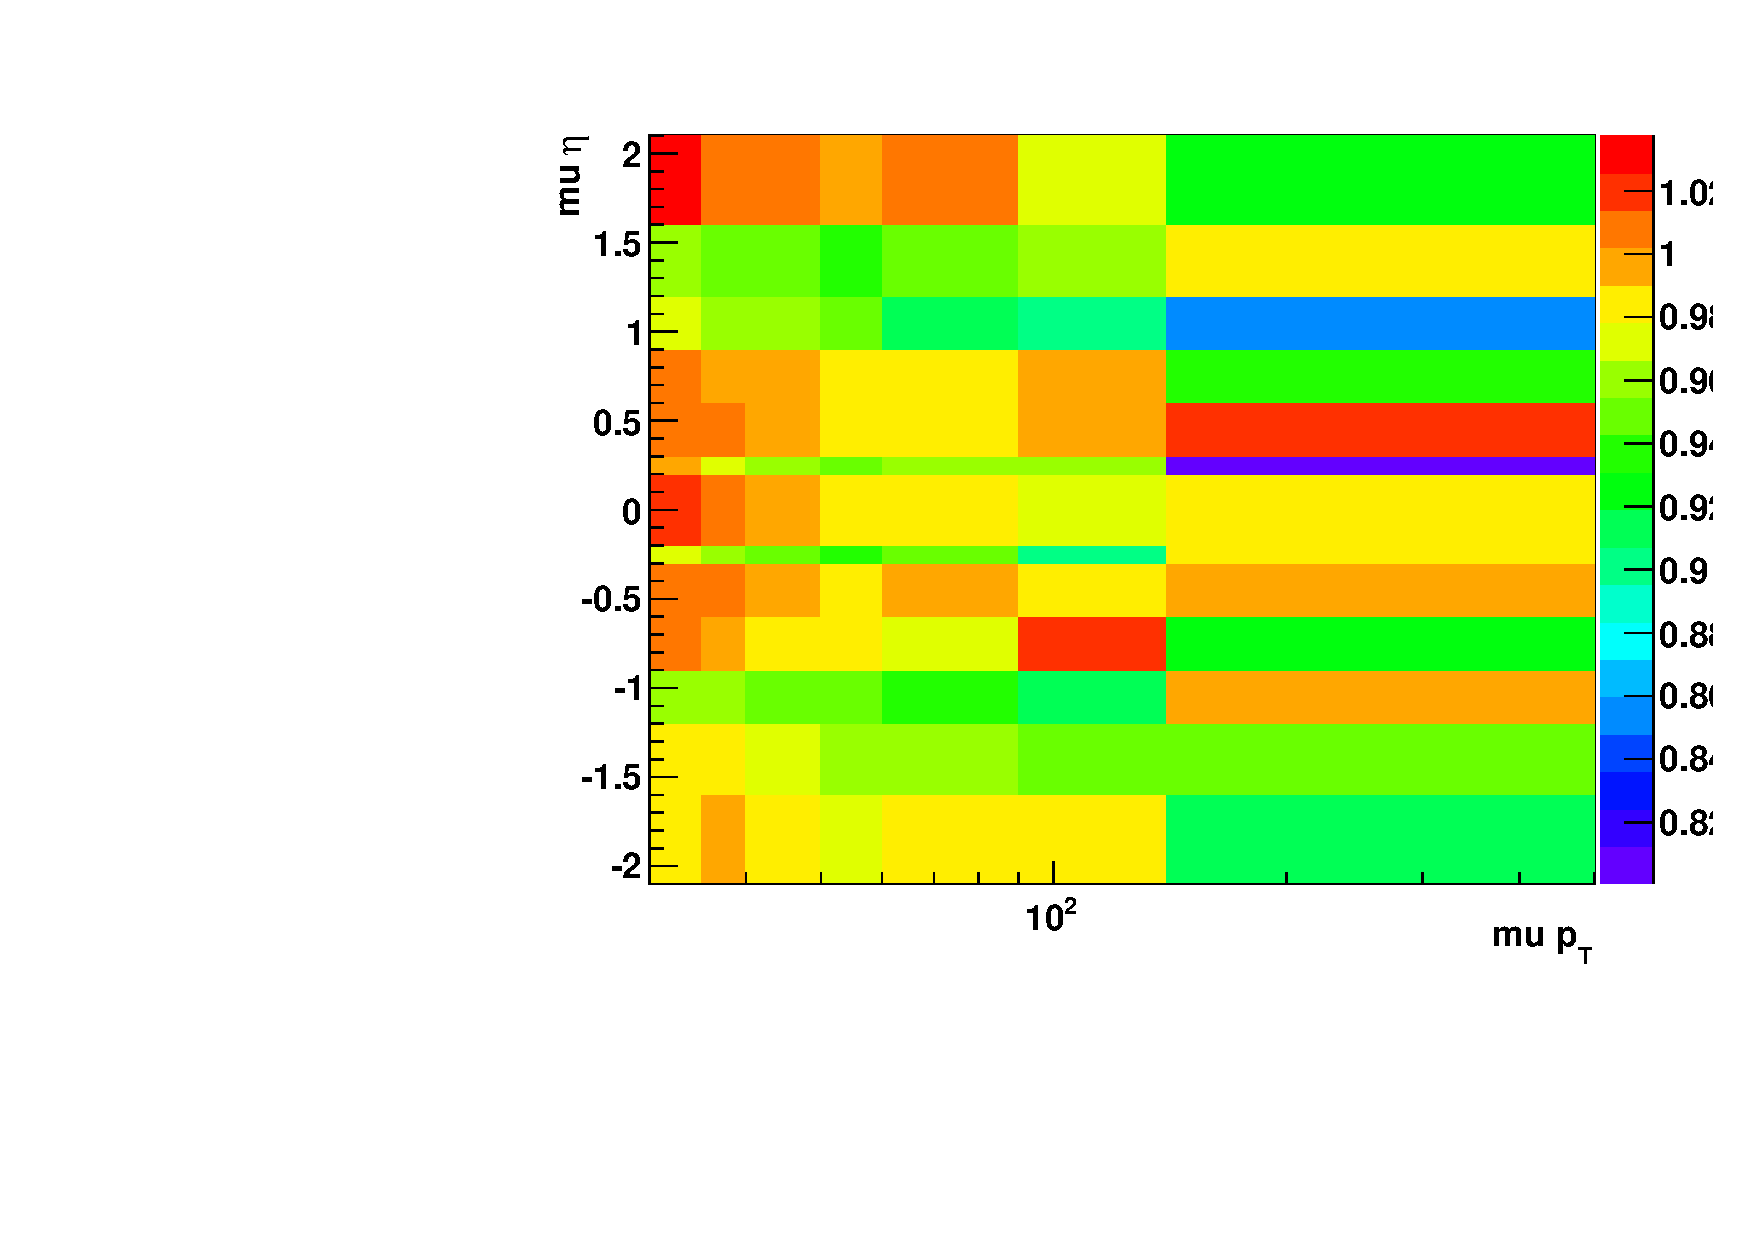
\includegraphics[width=0.45\textwidth]{Figures/Analysis_1_Diagrams/2d_mu_pt_eta_full_id_iso_hlt_data_over_mc.pdf}
   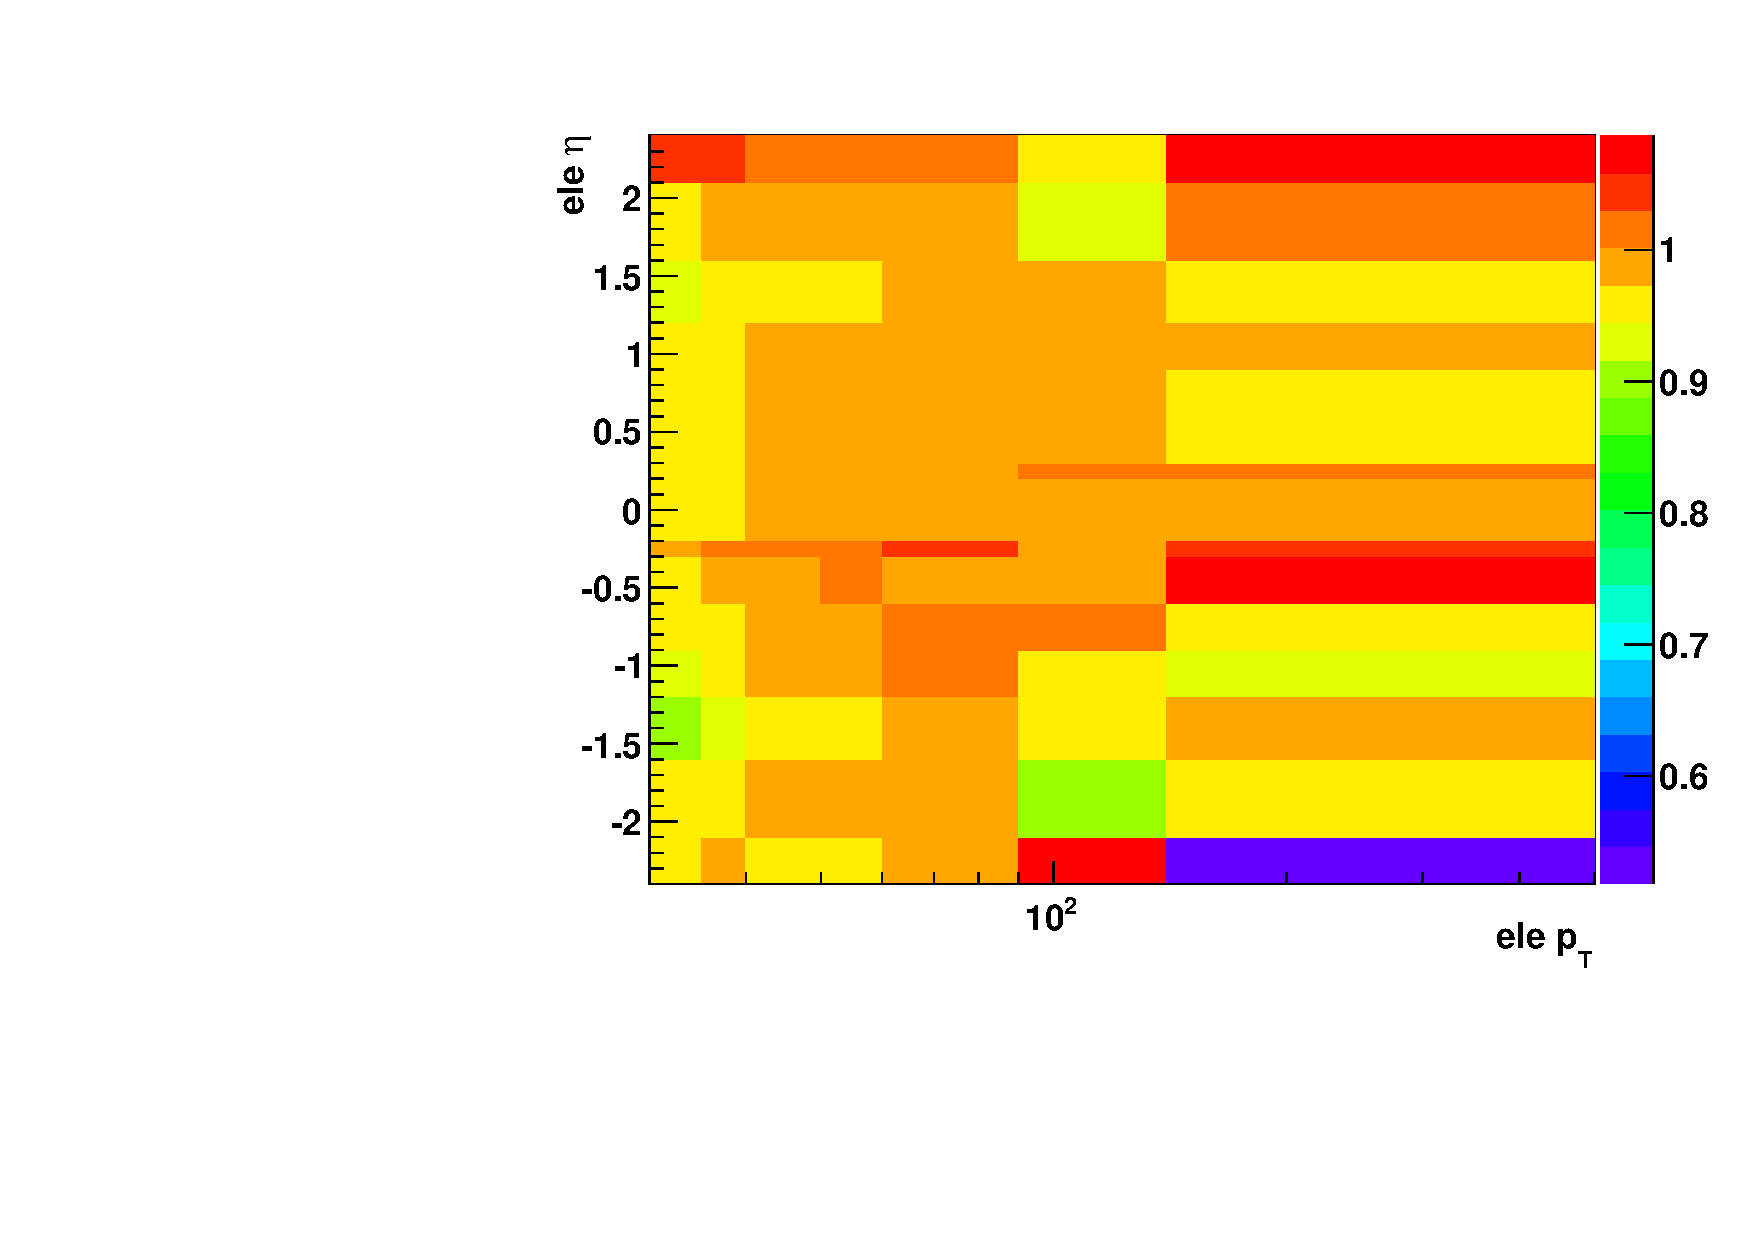
\includegraphics[width=0.45\textwidth]{Figures/Analysis_1_Diagrams/2d_ele_pt_eta_full_id_iso_hlt_data_over_mc.pdf}
   \caption{Muon and electron ID, isolation selection and trigger efficiency scale factors in bins of $p_{T}$ and $\eta$.}
   \label{fig:effSFHLT}
 \end{center}
\end{figure}

\par The combined ID, isolation, and trigger scale factor
uncertainty is evaluated by looking at the variation of the scale
factor as a function of parameters besides $p_T$ and $\eta$, such as
pileup and $b$-tag scale factor reweigting.  A flat uncertainty of 4$\%$
covers the variations that are observed, and is thus adopted as a
conservative estimate of the uncertainty on the combined lepton
reconstruction efficiency.  

\subsection{Jet selection}
\label{jet_selection_overview}

\par As described in the previous chapter, jets are reconstructed with
the anti-KT clustering algorithm~\cite{Cacciari:2008gp}, with a
distance parameter of of 0.5, starting from the set of objects
reconstructed by the particle flow algorithm
\cite{CMS-PAS-PFT-09-001}. Non-isolated leptons, not associated
with the decay of a $W$ boson, are allowed to be clustered into the
jets.  The selection cuts defining our jets can 
be found in Table~\ref{tab:JetTable}.  The cuts use the following
variables to ensure the reconstruction of authentic hadronic jets:

\begin{itemize}
  \item $p_{T}$ - component of the momentum transverse to the
    beam-line
  \item $\eta$ - the psuedorapidity of the reconstructed jet
  \item CEF - Charged Electromagnetic Fraction: the ratio of
    charged particles to the total number of particles in the jet
  \item NHF - Neutral Hadron Fraction: the ratio of neutral
    particles to the total number of particles in the jet
  \item NEF -  Neutral Electromangetic Fraction: the ratio of
    photons to the total number of particles in the jet
  \item CHF - Charged Hadron Fraction: the ratio of charged hadrons to
    the total number of particles in the jet
  \item NCH - Number of Charged Hadrons: raw charged hadron multiplicty
  \item N$_{constituents}$ - Number of constituents, which can be charged
  and neutral hadrons, as well as non-prompt photons and leptons.  
\end{itemize}

\begin{table}[hbtp]\footnotesize
\centering
\begin{tabular}{|l|c|c|}
\hline\hline
Cuts & Jet  \\
\hline
$p_{T}$ & \textgreater 30 GeV/c  \\
\hline
$|\eta|$ & \textless 2.4 \\
\hline
CEF, NHF, NEF & \textless 0.99 \\
\hline
CHF, NCH & \textgreater 0 \\
\hline
N$_{constituents}$ & \textgreater 1 \\
\hline\hline
\end{tabular}
\caption{Jet definition}
\label{tab:JetTable}
\end{table} 

\par Additional correction factors are required such that the measured
energy of the jet correctly reproduces the energy of the initial
parton.  This is done in four stages.  The L1 Charged Hadron
Subtraction (CHS) correction, is implemented in the particle-flow
algorithm, and involves subtracting the energy contributions from
charged hadrons that are not associated with the jet from the energy
cluster.  The next stage, L2 correction is a relative correction to
make the measured jet response flat in $\eta$.  The third stage, L3,
is an absolute correction to the measured $p_T$ of a jet in order to
match the simulated jet $p_{T}$ created using generator level input
and a similar jet clustering algorithm. The L2 and L3 corrections are
calculated using Monte Carlo, and thus an fourth correction factor,
the L2L3 residual correction is applied that fixes the discrepancies
between Monte Carlo and data.  The correction factors are described in
reference ~\cite{CMS:2011esa}, and are derived from 2011 7 TeV data,
with a selection of dijet events near the $Z$-boson mass peak.  A
"tag-and-probe'' procedure similar to the lepton scale factors is
applied to jets to determine the kinematic dependence ($p_{T}$ and
$\eta$) of the detector in both simulations and data.  Additionally, a
scale factor is needed to adjust for the difference in jet energy
resolution as measured in data and predicted in simulation.  Table
\ref{tab:JERtable} gives the scale factors, and uncertainties, as
derived from dijet events ~\cite{CMS:2011esa} as a function of $\eta$
only, since no signficant $p_{T}$ dependence was obsevered.  

\begin{table}
\centering
\begin{tabular}{|c|c|}
\hline\hline
$|\eta|$ & Data/MC Ratio \\ \hline
 & (factor +-stat. +syst.- syst.) \\ \hline
0.0–0.5 & 1.052$\pm$0.012+0.062-0.061 \\
0.5–1.1 & 1.057$\pm$0.012+0.056-0.055 \\
1.1–1.7 & 1.096$\pm$0.017+0.063-0.062 \\
1.7–2.3 & 1.134$\pm$0.035+0.087-0.085 \\
2.3–5.0 & 1.288$\pm$0.127+0.155-0.153 \\
\hline\hline
\end{tabular}
\caption{Jet Energy Resolution (JER) scale factors}
\label{tab:JERtable}
\end{table} 

\subsection{$b$-tagging selection}
\label{btag_overview}

\par The algorithm used to perform $b$-tagging in this analysis is the
combined secondary vertex (CSV) algorithm \cite{Weiser:927399}.  It
relies on the superior ability of the inner tracker to reconstruct
secondary vertices, which are the characteristic signature of
$b$-quark decays.  Tracks are selected is they meet the following
requirements: 
\begin{itemize}
  \item At least 8 hits in the pixel and silicon tracker, with at
    least 2 hits in the pixel detector
  \item tracks must have $p_{T}$>1 GeV
  \item $\chi^{2}$/NDF of the fitted track < 10
  \item $|d0|$ - transverse impact parameter < 2mm, since $b$-quarks
    will on average travel 0.45 mm in the detector before decaying
\end{itemize}

\noindent  Additionally, the following cuts are required:
\begin{itemize}
  \item The transverse distance between the primary and secondary
    vertices, $L_{T}$, is between 100 $\mu$m and 2.5 cm
  \item The ratio of $L_{T}$ and the uncertainty on it's measurement,
    $L_{T}/\sigma_{L_{T}}$>3 
  \item The invariant mass formed by adding the four-vectors of all
    the tracks forming the secondary vertex < 6.5 GeV
  \item The invariant mass falls outside a window near 50 MeV,
    corresponding to the $K_{S}^{0}$ resonance
\end{itemize}

\noindent  Secondary vertices are decomposed into three categories.
If a secondary vertex is found meeting the above criteria, it is a
"reco vertex''.  If no secondary vertex is found meeting all the above
criteria, the event can be classified as a "psuedo vertex'' if more
than two tracks have a signed transverse impact parameter
significance, relative to the primary vertex, greater than 2.  "No
vertex'' is found if neither of the prior two classification criteria
can be met.  
 
\par For each of the vertex categories, a set of variables is used to
create a single discriminating variable, using a likelihood ratio
technique.  The following input variables are used:
\begin{itemize}
  \item The invariant mass of the charged particles assoicated with
    the secondary vertex
  \item The multiplicity of charged tracks associated with the primary
    vertex
  \item The distance between the primary and secondary vertex in the
    transverse plane, divided by its error (only used in reco vertex category)
  \item The psuedorapidities of the charged particle tracks associated
    with the secondary vertices
  \item The track impact parameter significance of the highest $p_{T}$
    track with invariant mass larger than the charm quark threshold,
    1.5 GeV. 
\end{itemize}

\noindent The likelihood function is split to seperate between the
charm and light-flavour backgrounds and is defined as:

\begin{equation}\label{eq:csv_likelihood}
\mathcal{L}^{b,c,q} =
f^{b,c,q}(\alpha)\times\prod_{i}f_{\alpha}^{b,c,q}(x_{i})
\end{equation}

\noindent where $\alpha$ = 1,2,3, denotes the different vertex
categories, $x_{i}$ are the individual variables, $q$ stands for the
light flavour quarks, while $b$ and $c$ stand for the bottom and charm
quarks resepctively.  $f^{b,c,q}(\alpha)$ is the probabilty for a
quark flavour $b,c,$ or $q$, to fall into category $\alpha$.
$f_{\alpha}^{b,c,q}(x_{i})$ is the probabiltiy deensity
function of the variable $x_{i}$ in catgory $\alpha$ for quark flavour
$b,c,$ or $q$.  The combined descriminate is defined as

\begin{equation}\label{eq:csv_disc}
d = f_{BG}(c)\times\frac{\mathcal{L}^{b}}{\mathcal{L}^{c} +
  \mathcal{L}^{b}} + f_{BG}(q)\times\frac{\mathcal{L}^{b}}{\mathcal{L}^{q} +
  \mathcal{L}^{b}}
\end{equation}

\noindent where $f_{BG}(c)$, and $f_{BG}(q)$ are
the a-priori probabilities for the content of charm and light flavour
quarks in non-b jets.  

\par A jet is considered $b$-tagged if the CSV discriminant is greater
than 0.679, which is the medium working point defined by the BTag
Physics Object Group (POG)~\cite{btagOP}, defined in order to produce
a light-flavour mistag rate at $\sim1\%$, with the reconstruction
efficiency for real b-jets at $\sim70\%$.  

\par Additionally, it is necessary to account for differences in the
measured efficiency for $b$-tagging jets between data and
simulation~\cite{CMS-PAS-BTV-11-004}.
An event weight scale factor is used to correct the MC $b$-tagging efficiency ($SF_{tag} =
\epsilon_{tag}^{data}/\epsilon_{tag}^{MC}$).  The scale factor is
measured for three different cuts, or working points, on the CSV
discriminant value, and it is binned in terms of the $p_{T}$ and
$\eta$ and flavour of the jet.  

\par In addition to providing jet flavour identification for event
classification, the discriminant value of the algorithm will be used
to seperate between \ttH signal and \ttjets background.  Therefore, a
correction value for the efficiency difference between data and MC over the whole range
of discriminator values is needed, not just for three working points.
This procedure was developed in the context of the search for the
standard model Higgs boson produced in association with a W or Z
boson, with the Higgs decaying to bottom
quarks~\cite{CMS-AN-2012-181}.  

\par For each of the three operating points and for each of the
data/MC SFs, an equivalent cut on the CSV value is determined,
\(CSV_{\mathrm{equiv}}\), such that 

\begin{equation}\label{eq:csv_reweight}
\epsilon^{data}_{CSV>CSV_{\mathrm{orig}}} = SF_{CSV>CSV_{\mathrm{orig}}}\cdot\epsilon^{MC}_{CSV>CSV_{\mathrm{orig}}} = \epsilon^{MC}_{CSV>CSV_{\mathrm{equiv}}}
\end{equation}

\noindent where the SFs are measured in data and the MC efficiency
measurements are calculated for each sample.

\par In order to correct or "reshape'' the CSV discriminator output
values, a function is applied to the MC to produces a corrected CSV value:
$CSV_{\mathrm{corr}}=f(CSV_{\mathrm{orig}})$.  Given that there are
three $b$-tag efficiency measurements, there are three pairs of
($CSV_{\mathrm{orig}}$, $CSV_{\mathrm{equiv}}$). The reshaping
function must satisfy $f(CSV_{\mathrm{equiv}}) =
CSV_{\mathrm{orig}}$ for each of the operating points and for the upper
and lower values of the CSV discriminant to make sure those values do
not change (e.g., $CSV = 0.0$ and $CSV = 1.0$).  The whole range of
CSV discriminant values is found by linearly interpolating between
these five points (the three working points, and upper and lower limit
of the discrimant range).


\subsection{Lepton + Jets Selection}
\label{LJ_selection_overview}

\par The final Lepton+Jets (LJ) selection is finally carried out by
requiring that events have exactly one tight lepton ($e$ or
$\mu$), and at least four jets. Eevents with any additional loose or
tight leptons are vetoed so this analysis can later be combined with a
diLepton final state, without double counting events. Additionally,
each event must have at least three jets with $p_{T} > 40$ GeV/c.

\par Events are further catergorized by the reconstructed jet, and
$b$-tagged jet multiplicities as follows:

\begin{itemize}
  \item $\ge$6 jets,  $==$2 $b$-tags: At least 6 jets, 2 of which are $b$-tagged 
  \item $==$4 jets, $==$3 $b$-tags: Exactly 4 jets, 3 of which are $b$-tagged 
  \item $==$5 jets, $==$3 $b$-tags: Exactly 5 jets, 3 of which are $b$-tagged 
  \item $\ge$6 jets, $==$3 $b$-tags: At least 6 jets, 3 of which are $b$-tagged 
  \item $==$4 jets, $==$4 $b$-tags: Exactly 4 jets, 4 of which are $b$-tagged 
  \item $==$5 jets, $==$4 $b$-tags: Exactly 5 jets, 4 of which are $b$-tagged 
  \item $\ge$6 jets, $\ge$4 $b$-tags: At least 6 jets, with at least 4 of which are $b$-tagged 
\end{itemize}

\noindent Events with either 4 or 5 jets, where 2 of the those jets
are $b$-tagged, make up two categories, which are used only as a
control region to validate comparisons between collected data and
simulations.  The number of $t\bar{t}H$ events increases with the
number of jets and tags because the largest branching fraction is $H$
to $b\bar{b}$.  Data to monte carlo comparisons of the jet and $b$-tag
multiplicities are shown in figure \ref{fig:njetsntags_LJ}.  The event
yields for the $\mu$+jets and $e$+jets channels are shown in tables
\ref{tab:dataMC_LJeventyield_mu} and \ref{tab:dataMC_LJeventyield_ele}
respectively. 

\begin{figure}[hbtp!]
 \begin{center}
   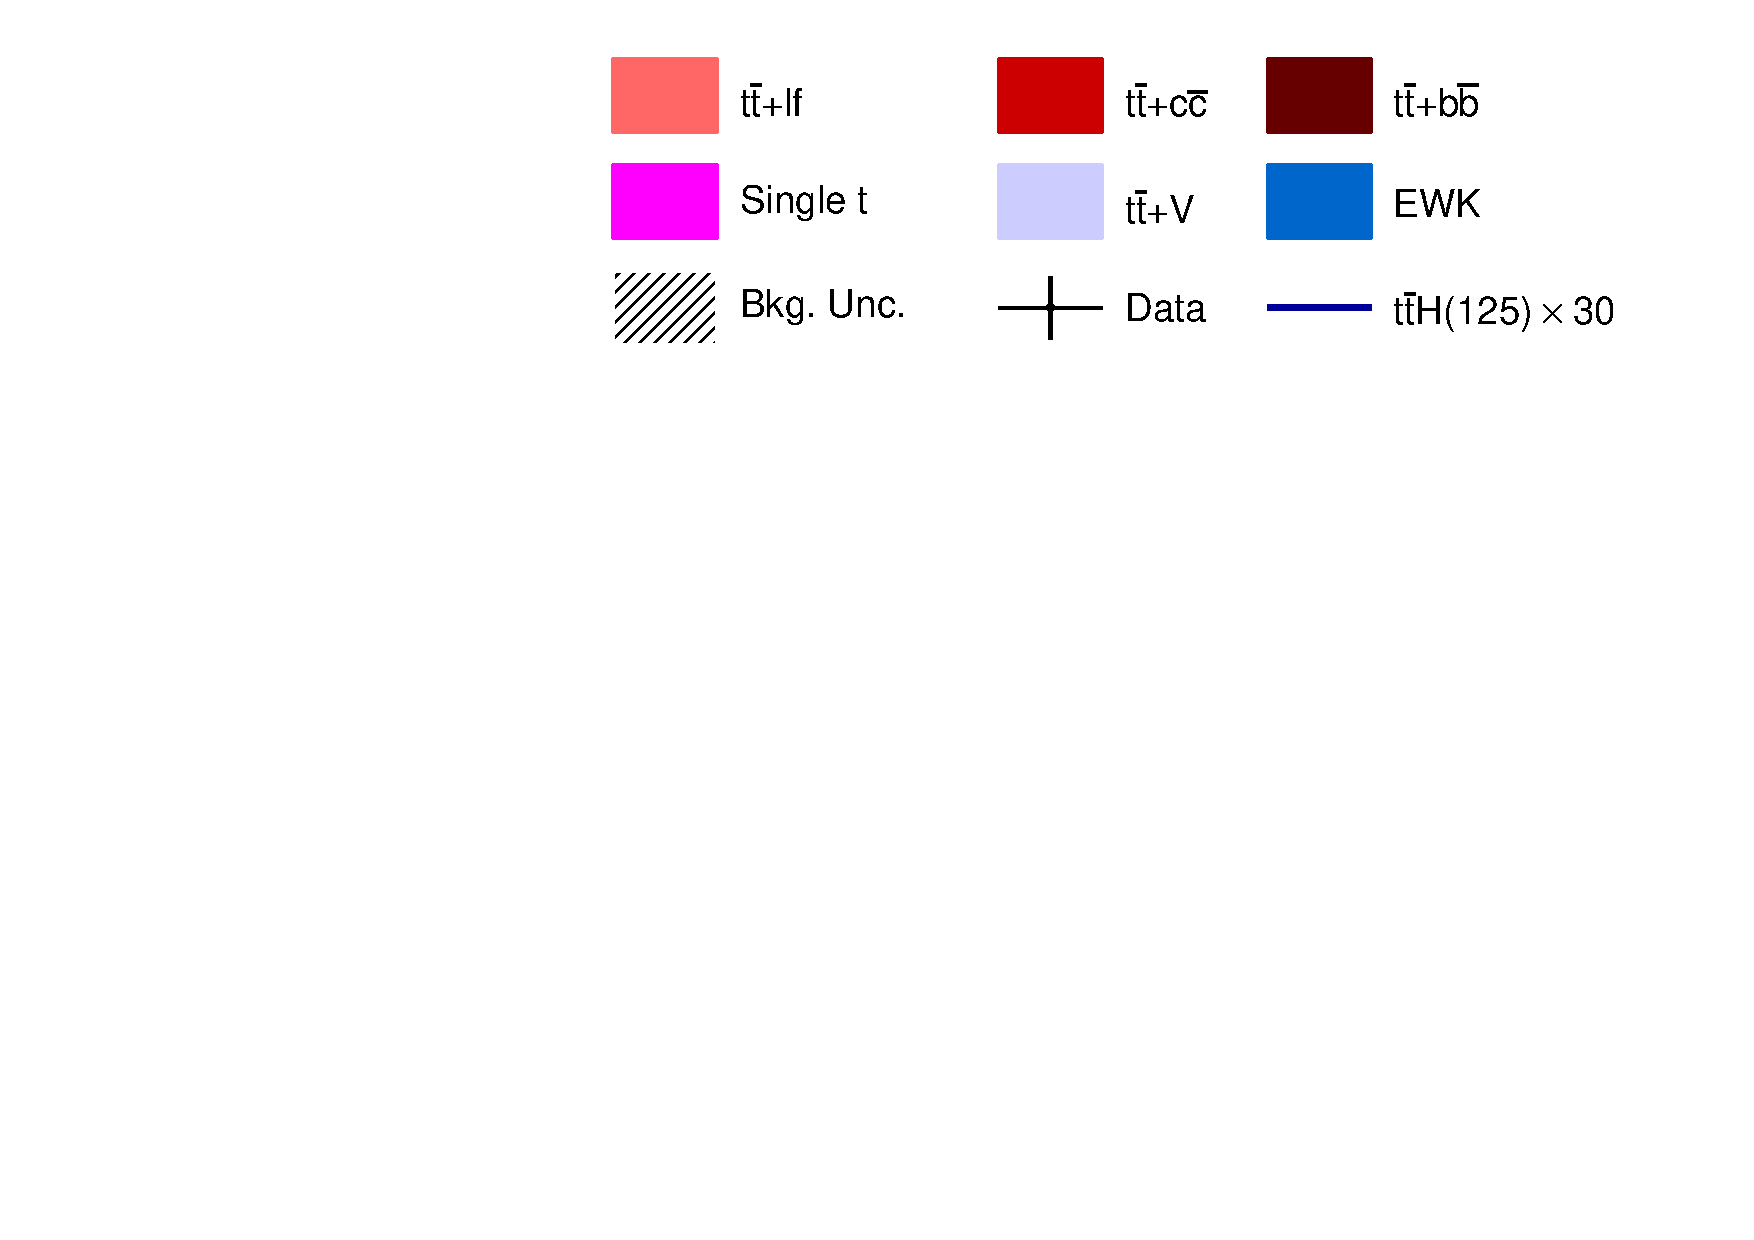
\includegraphics[width=0.60\textwidth]{Figures/Analysis_1_Diagrams/samples_legend_wide.pdf} \\
   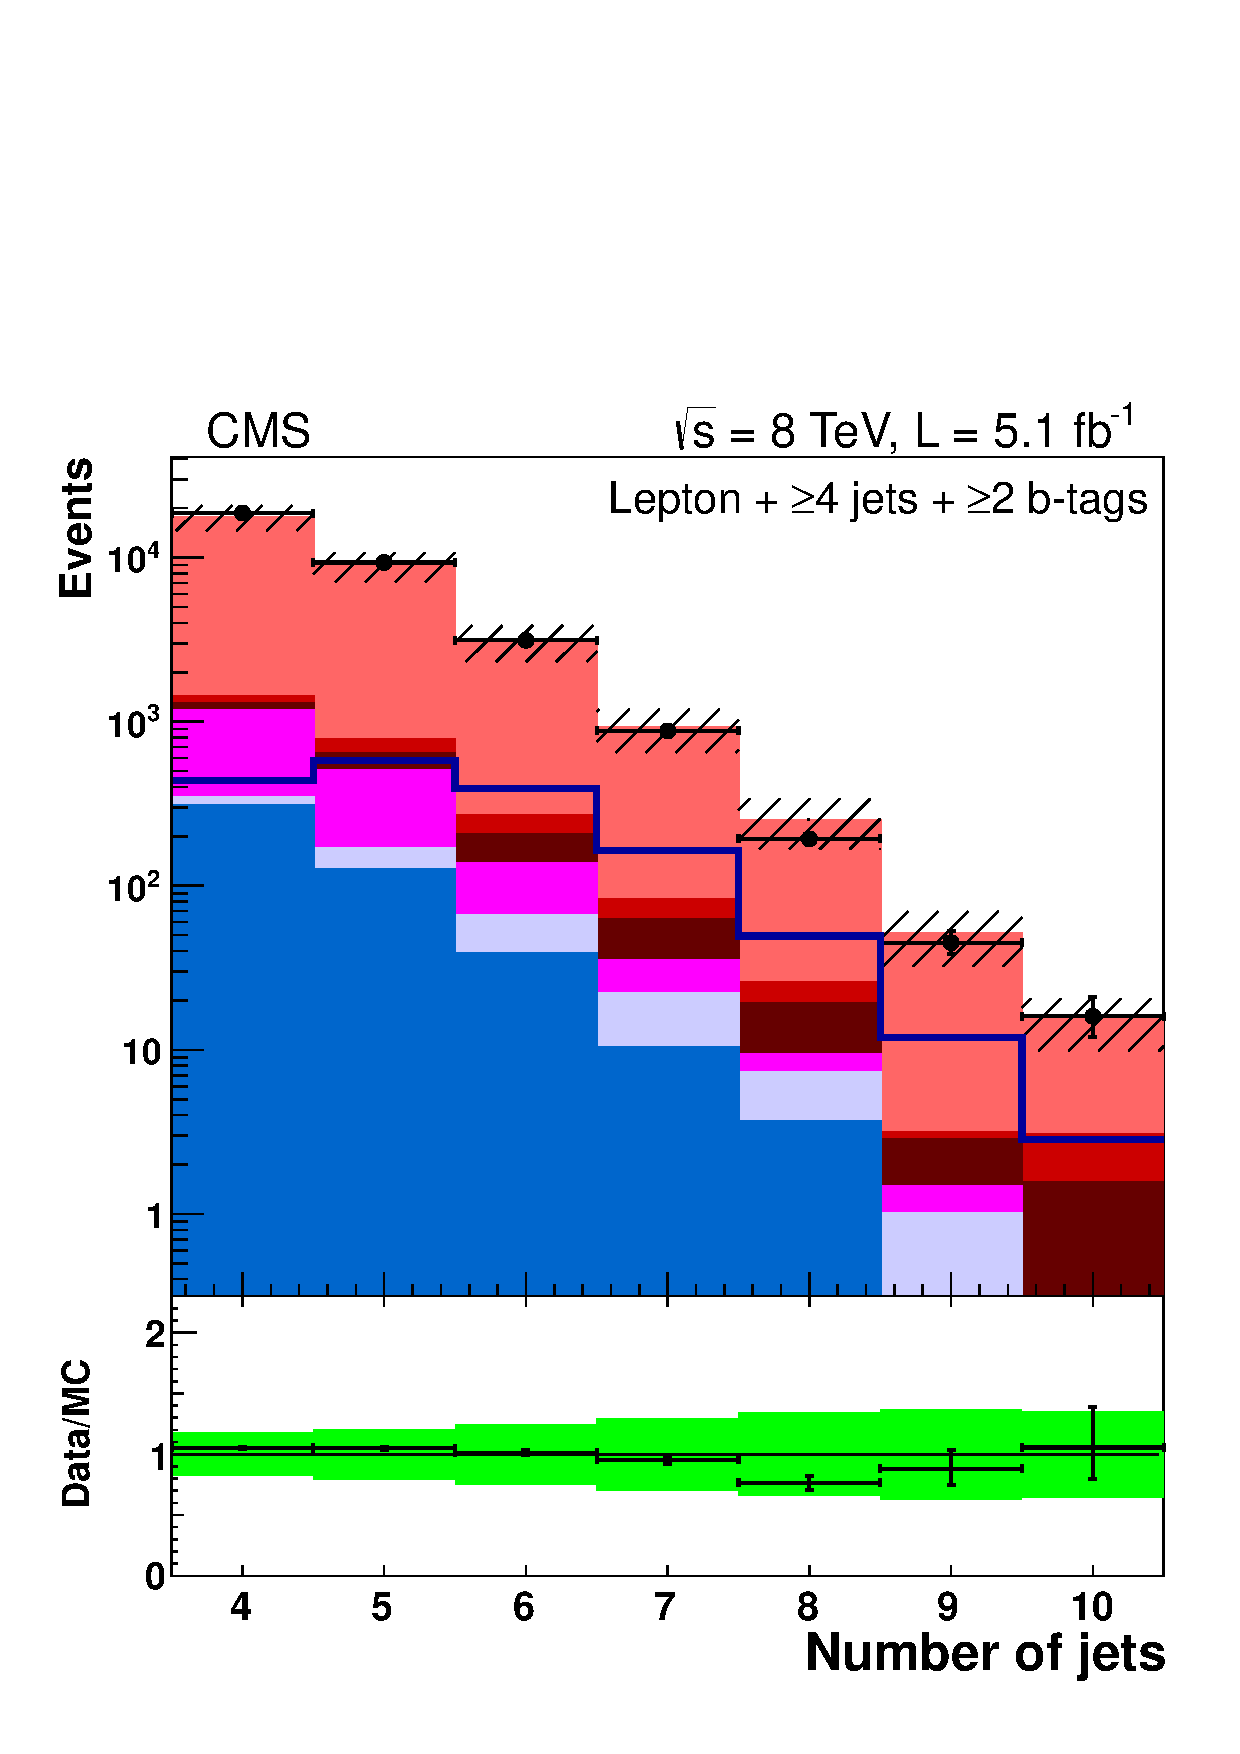
\includegraphics[width=0.35\textwidth]{Figures/Analysis_1_Diagrams/d2MCPlots_numJets_cut0_jge4_tge2_Combined_HtWgt.pdf}
   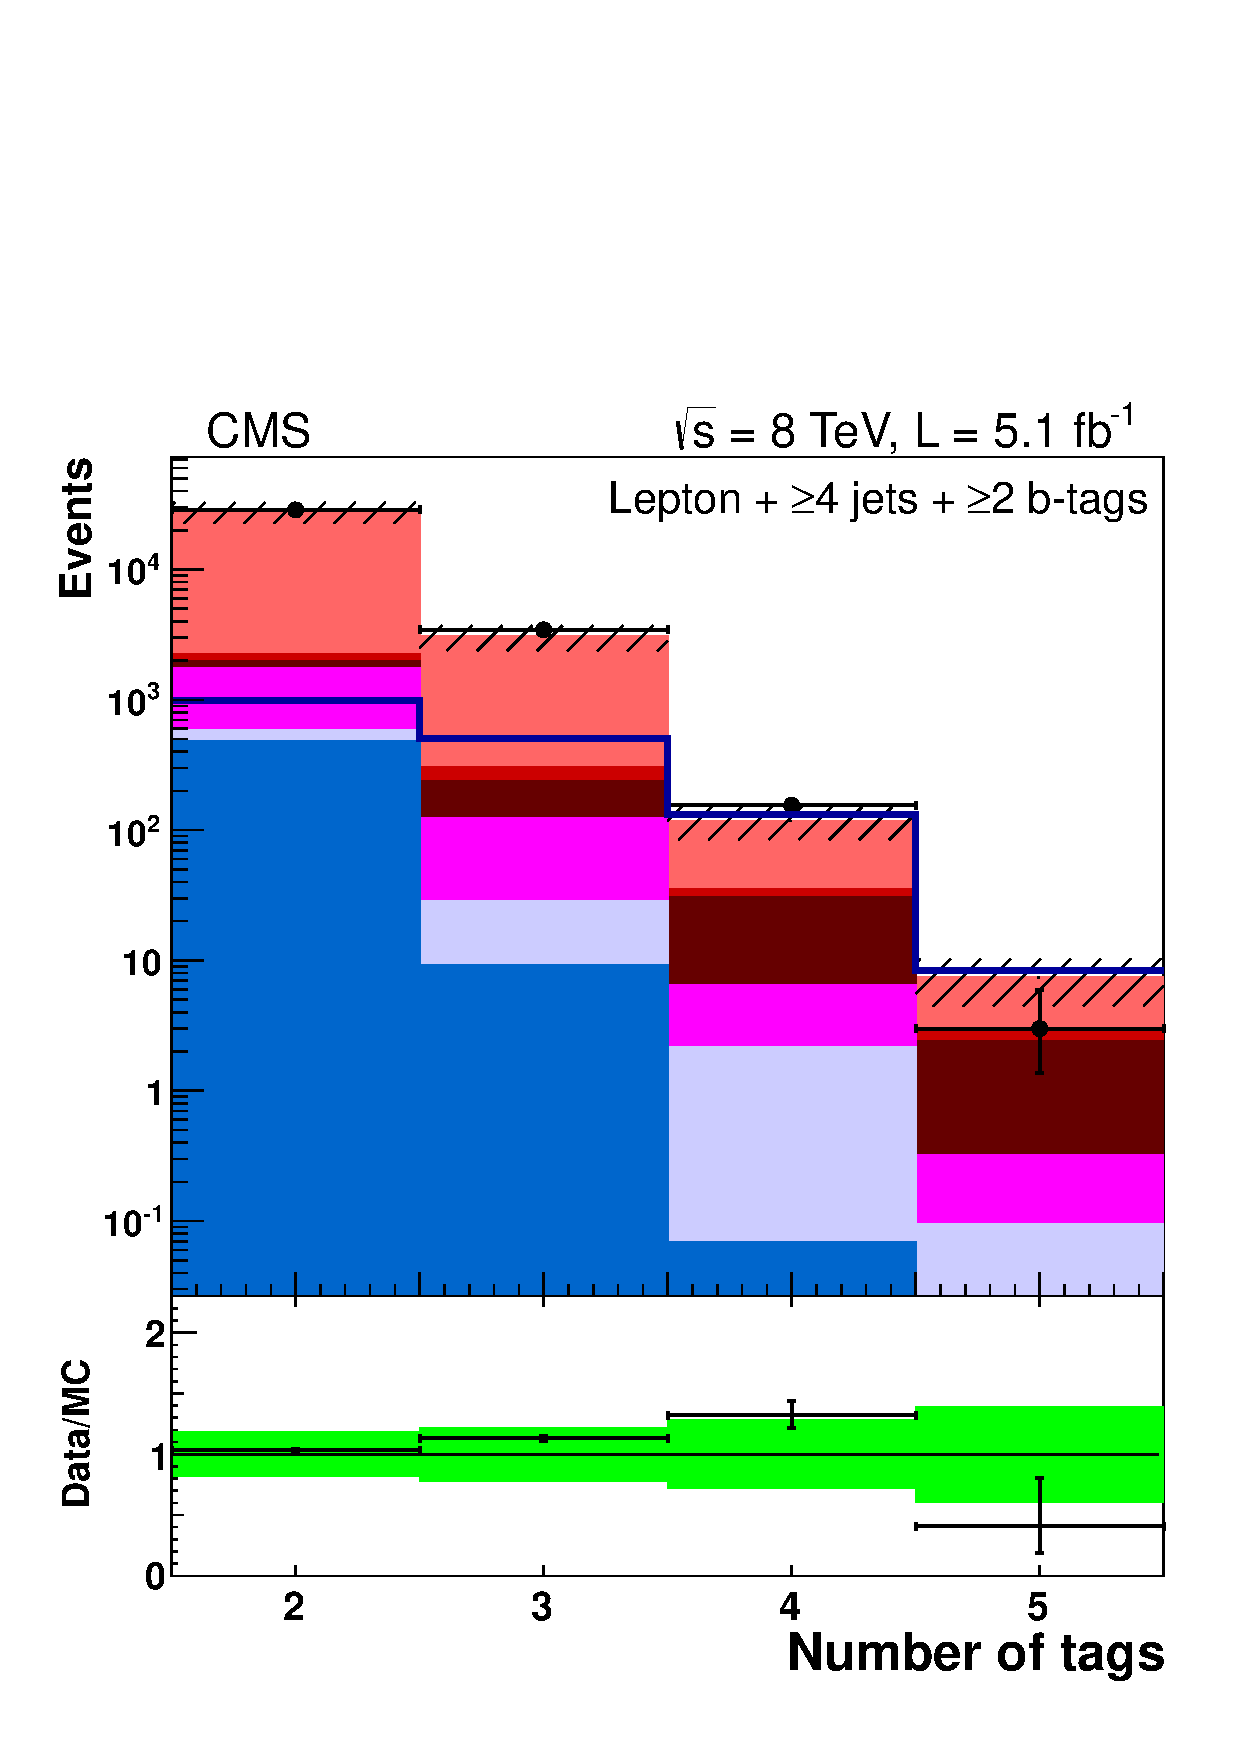
\includegraphics[width=0.35\textwidth]{Figures/Analysis_1_Diagrams/d2MCPlots_numTags_cut0_jge4_tge2_Combined_HtWgt.pdf}
   \caption{Number of jets (left) and number of b-tagged jets
   (right) in data and simulation for events with $\ge$4~jets +
   $\ge$2~b-tags in the lepton+jets channel at $8 \TeV$. The
   background is normalized to the SM expectation; 
   the uncertainty band (shown as a hatched band in the
   stack plot and a green band in the ratio plot) includes statistical
   and systematic uncertainties that affect both the rate and shape of
   the background distributions.  The $\ttH$ signal ($m_{H} =                                                                                                  
   125 \GeVcc$) is normalized to 30 $\times$ SM expectation.}
   \label{fig:njetsntags_LJ}
 \end{center}
\end{figure}

\begin{sidewaystable}[h]
\begin{adjustwidth}{-1.7in}{-1.7in}
  \centering
  \noindent
  \small
    \caption{Expected event yields in 5 fb$^{-1}$ for signal and backgrounds in the $\mu$+jets channel.}
    \label{tab:dataMC_LJeventyield_mu}
    \begin{tabular}{|l|c|c|c|c|c|c|c|} \hline
& $\geq$6 jets & 4 jets & 5 jets & $\geq$6 jets & 4 jets & 5 jets & $\geq$6 jets \\
& 2 tags & 3 tags & 3 tags & 3 tags & 4 tags & $\geq$4 tags & $\geq$4 tags \\ \hline \hline
$t\bar{t}H(125)$ & 6.1 $\pm$ 1.1 & 2.1 $\pm$ 1.9 & 3.2 $\pm$ 2.7 & 3.6 $\pm$ 3.3 & 0.3 $\pm$ 0.3 & 0.8 $\pm$ 0.9 & 1.3 $\pm$ 1.4 \\
 \hline
$t\bar{t}+$lf & 1750 $\pm$ 480 & 680 $\pm$ 150 & 460 $\pm$ 110 & 270 $\pm$ 84 & 9.5 $\pm$ 3.2 & 13.0 $\pm$ 4.2 & 20.6 $\pm$ 7.8 \\
$t\bar{t}+b\bar{b}$ & 34 $\pm$ 19 & 21 $\pm$ 12 & 24 $\pm$ 14 & 17.3 $\pm$ 10.0 & 1.5 $\pm$ 1.1 & 5.1 $\pm$ 3.2 & 8.6 $\pm$ 5.6 \\
$t\bar{t}+c\bar{c}$ & 29.5 $\pm$ 8.7 & 10.0 $\pm$ 2.9 & 13.2 $\pm$ 3.9 & 11.1 $\pm$ 3.5 & 0.2 $\pm$ 0.2 & 0.2 $\pm$ 0.1 & 1.1 $\pm$ 0.8 \\
$t\bar{t}V$ & 18.7 $\pm$ 3.9 & 2.3 $\pm$ 0.6 & 3.3 $\pm$ 0.8 & 4.1 $\pm$ 1.1 & 0.1 $\pm$ 0.0 & 0.4 $\pm$ 0.2 & 0.8 $\pm$ 0.2 \\
Single $t$ & 42.6 $\pm$ 9.8 & 25.8 $\pm$ 6.0 & 14.3 $\pm$ 3.8 & 4.3 $\pm$ 1.3 & 0.2 $\pm$ 0.3 & 1.6 $\pm$ 1.8 & 0.7 $\pm$ 0.5 \\
$V+$jets & 39 $\pm$ 32 & 1.0 $\pm$ 0.9 & 0.0 $\pm$ 0.0 & 0.0 $\pm$ 0.0 & 0.0 $\pm$ 0.0 & 0.0 $\pm$ 0.0 & 0.0 $\pm$ 0.0 \\
Diboson & 0.6 $\pm$ 0.2 & 0.9 $\pm$ 0.4 & 0.3 $\pm$ 0.1 & 0.1 $\pm$ 0.1 & 0.0 $\pm$ 0.0 & 0.0 $\pm$ 0.0 & 0.0 $\pm$ 0.0 \\
 \hline
Total bkg & 1910 $\pm$ 500 & 740 $\pm$ 160 & 520 $\pm$ 120 & 307 $\pm$ 90 & 11.4 $\pm$ 3.8 & 20.3 $\pm$ 6.1 & 32 $\pm$ 11 \\
 \hline
Data & 1780 & 861 & 585 & 362 & 15 & 32 & 37 \\
\hline
\end{tabular}
\vspace{10 mm}
  \noindent
  \small
    \caption{Expected event yields in 5 fb$^{-1}$ for signal and backgrounds in the $e$+jets channel.}
    \label{tab:dataMC_LJeventyield_ele}
    \begin{tabular}{|l|c|c|c|c|c|c|c|} \hline
& $\geq$6 jets & 4 jets & 5 jets & $\geq$6 jets & 4 jets & 5 jets & $\geq$6 jets \\
& 2 tags & 3 tags & 3 tags & 3 tags & 4 tags & $\geq$4 tags & $\geq$4 tags \\ \hline \hline
$t\bar{t}H(125)$ & 5.6 $\pm$ 1.0 & 1.8 $\pm$ 1.2 & 2.9 $\pm$ 1.8 & 3.2 $\pm$ 2.1 & 0.3 $\pm$ 0.2 & 0.7 $\pm$ 0.6 & 1.2 $\pm$ 1.0 \\
 \hline
$t\bar{t}+$lf & 1720 $\pm$ 470 & 640 $\pm$ 140 & 410 $\pm$ 94 & 293 $\pm$ 85 & 8.6 $\pm$ 2.9 & 14.5 $\pm$ 5.2 & 20.7 $\pm$ 7.8 \\
$t\bar{t}+b\bar{b}$ & 27 $\pm$ 15 & 14.3 $\pm$ 7.9 & 19 $\pm$ 11 & 18 $\pm$ 10 & 1.0 $\pm$ 1.0 & 3.3 $\pm$ 2.6 & 6.7 $\pm$ 4.3 \\
$t\bar{t}+c\bar{c}$ & 32.8 $\pm$ 9.4 & 9.6 $\pm$ 2.9 & 11.8 $\pm$ 3.5 & 14.8 $\pm$ 4.8 & 0.4 $\pm$ 0.3 & 0.6 $\pm$ 0.6 & 2.6 $\pm$ 1.4 \\
$t\bar{t}V$ & 17.0 $\pm$ 3.6 & 2.1 $\pm$ 0.6 & 2.8 $\pm$ 0.7 & 4.5 $\pm$ 1.1 & 0.0 $\pm$ 0.0 & 0.3 $\pm$ 0.1 & 0.6 $\pm$ 0.2 \\
Single $t$ & 35.9 $\pm$ 8.9 & 30.5 $\pm$ 6.4 & 11.3 $\pm$ 3.4 & 6.0 $\pm$ 2.0 & 0.1 $\pm$ 0.3 & 1.4 $\pm$ 1.2 & 0.4 $\pm$ 0.4 \\
$V+$jets & 14 $\pm$ 14 & 4.8 $\pm$ 5.8 & 0.8 $\pm$ 0.9 & 0.0 $\pm$ 0.0 & 0.0 $\pm$ 0.0 & 0.0 $\pm$ 0.0 & 0.0 $\pm$ 0.0 \\
Diboson & 0.7 $\pm$ 0.3 & 1.0 $\pm$ 0.3 & 0.2 $\pm$ 0.1 & 0.1 $\pm$ 0.0 & 0.0 $\pm$ 0.0 & 0.0 $\pm$ 0.0 & 0.0 $\pm$ 0.0 \\
 \hline
Total bkg & 1850 $\pm$ 490 & 700 $\pm$ 150 & 460 $\pm$ 110 & 336 $\pm$ 93 & 10.1 $\pm$ 3.2 & 20.2 $\pm$ 6.6 & 31 $\pm$ 11 \\
 \hline
Data & 1723 & 785 & 531 & 324 & 13 & 24 & 37 \\
\hline
\end{tabular}
  \end{adjustwidth}
\end{sidewaystable}



\section{Multivariate Analysis}
\label{mva_overview}

\par As discussed in the chapter introduction, no single variable
offers sufficient discriminating power, to seperate the \ttH signal
from the \ttjets background.  Instead, the combined power of several
input variables is utilized through a multivariate analysis (MVA)
technique.  For this analysis, the MVA algorithm chosen from the sub-class
of artifical neural network (ANN) algorithms, known as multi-layer
perceptrons (MLPs).  The specific algorithm is the Clermond-Ferrand
Multi-Layer Perceptron Artificial Neural Network (CFMlpANN).  It was
first developed at the Universit´e Blaise Pascal in Clermont-Ferrand,
for the ALEPH experiment at the LEP collider to search for the
Standard Model Higgs and has also been utilized by the BABAR
experiment to search for rare $B$ meson decays \cite{Hocker:2007ht}.
It has been implemented in the ROOT TMVA framework, available in all
CMSSW releases.  A CFMlpANN is trained for each jet-tag category
listed in section \ref{LJ_selection_overview}.  A total of 10 input
variables is used in each category, with the exception of the $\ge$6
jets, $\ge$4 $b$tags category, where the full reconstruction of the
\ttH system is possible, features an additional variable that is the
invariant mass of the di-jet system of $b$-jets selected by a
$\chi^{2}$ minimization algorithm.  

\subsection{Artificial Neural Network Overview}
\label{ann_overview}

\par An artificial neural network (ANN), most generally speaking, is
any collection of interconnected, simulated "neurons'' which produce a
certain response to a set of input variables \cite{Hocker:2007ht}.  A
simulated neuron, is some independent function, which takes several
input variables, performs a mathematical operation, and passes the
result to one or more other neurons.  In the most general case, a set
of $n$ input variables, connected to a single output, will produce on
the order $n^{2}$ connections.  For case of using the network to
discriminate between signal from background (a yes or no answer on
whether an event is signal-like), the ANN is mapping an
$n$-dimensional space onto a one-dimensional space.  

\begin{figure}[hbtp]
 \begin{center}
   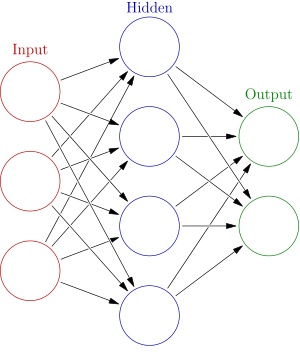
\includegraphics[width=0.45\textwidth]{Figures/Analysis_1_Diagrams/ANN_simple.png}
   \caption{A simple example of a MLP type ANN, with one layer of
     input neurons that make connections to a hidden layer, which is
     connected to the output layer}
   \label{fig:mlp_simple}
 \end{center}
\end{figure}

\par The multi-layer perceptron (MLP) is a specific type of
arrangement of neurons.  Any number of nuerons are arranged into a
single layer, and connections to other neurons are only made if they
are arranged in a successive layer \cite{Hocker:2007ht}.  This is
known as feed-forward network, and a simple example with one input
layer, one hidden layer, and one output layer is shown in figure
\ref{fig:mlp_simple}.  This limits the complexity of the connections
formed by the neurons and allows for simplified calculations.  

\begin{figure}[hbtp]
 \begin{center}
   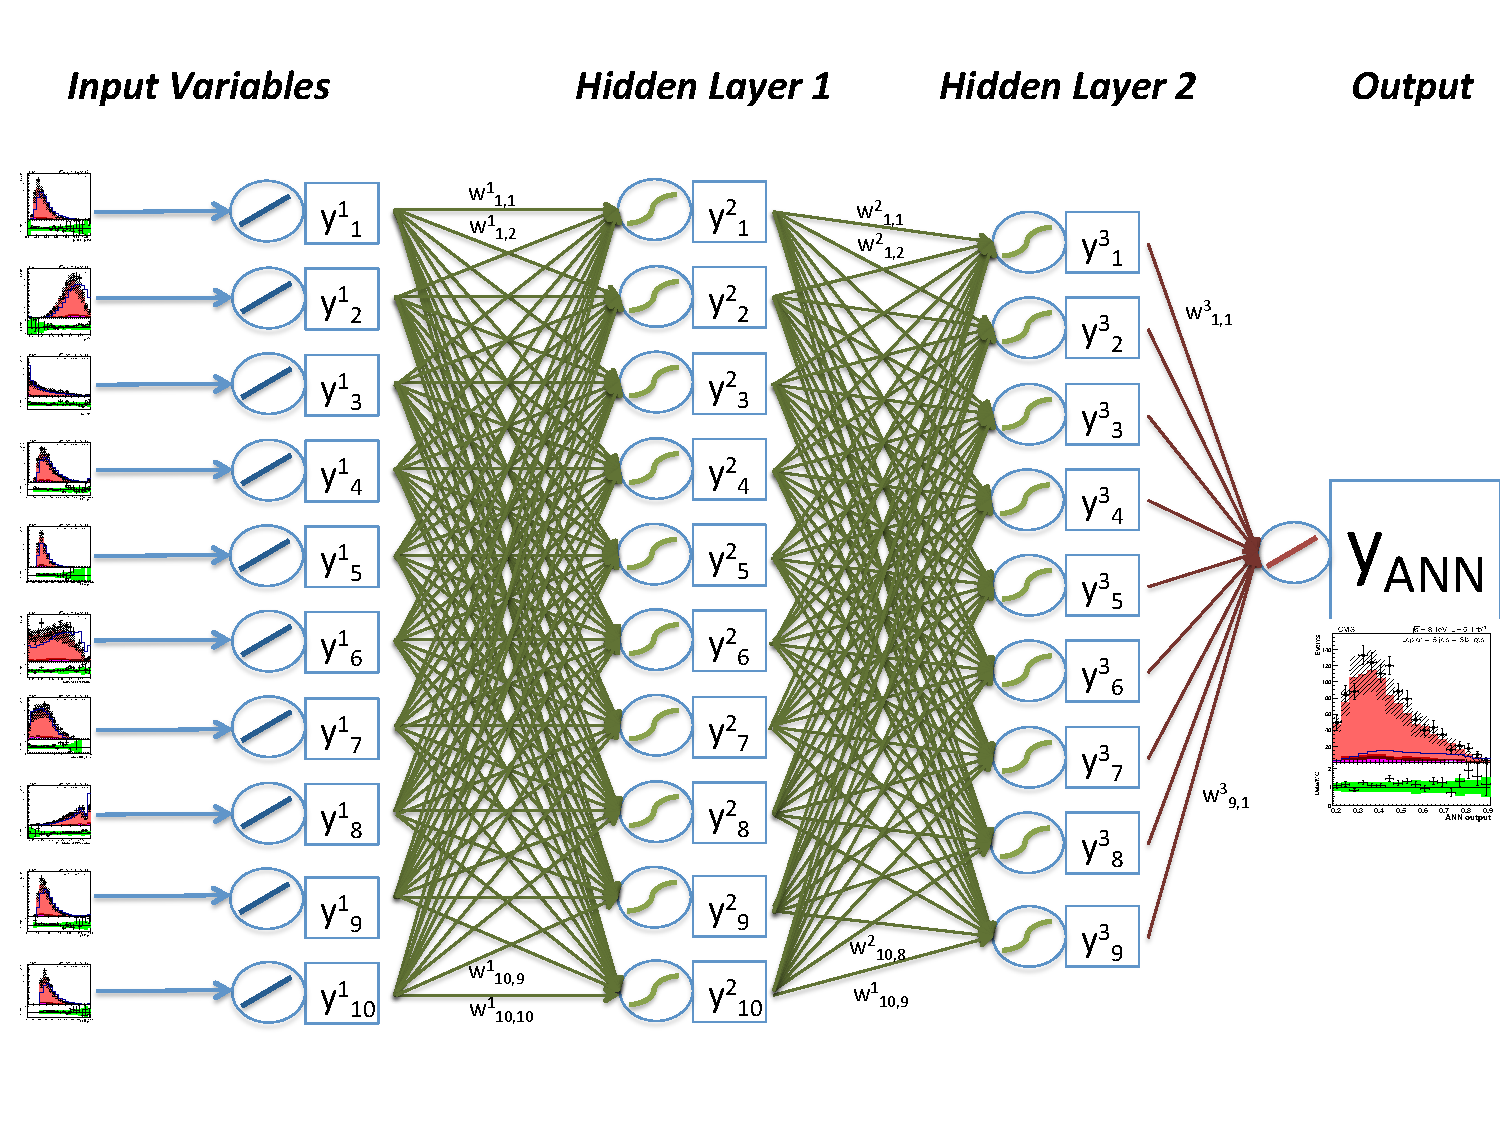
\includegraphics[width=1.0\textwidth]{Figures/Analysis_1_Diagrams/CFMlpANN_Architecture.pdf}
   \caption{The CFMlpANN architechture used in this analysis features
     two hidden layers, and 10 input variables for each jet/tag
     category (11 variables for the $\ge$6jets, $\ge$4$b$-tags
     category)}
   \label{fig:cfmlpann_arch}
 \end{center}
\end{figure}

\par This analysis uses an architecture that consists of two hidden
layers, with $N$ and $N-1$ variables respecitvely, where $N$ is the
number of input variables for the given jet/tag category.  An example
diagram is shown in figure \ref{fig:cfmlpann_arch}.  The output of the
CFMlpANN algorithm is one-dimensional discriminant with range from 0
to 1, for background-like and signal-like events.  Each neuron
response is the based on an activation function $A(\alpha)$, and a synapse
repsonse, $\alpha$.  In this case, a sigmoid function is used as
the activation function:

\begin{equation}\label{eq:sigmoid}
A(\alpha) = \frac{1}{1+e^{-x}}
\end{equation}

\noindent and the synapse response is a simple weighted sum:

\begin{equation}\label{eq:ann_synapse}
\alpha = w_{0j}^{(l)} + \sum_{i=1}^{n}y_{i}^{(l)}w_{ij}^{(l)} 
\end{equation}

\noindent The entire CFMlpANN response is then 

\begin{equation}\label{eq:ann_output}
y_{ANN} = \sum_{k=1}^{n-1}y_{k}^{(3)}w_{k1}^{(3)} = \sum_{k=1}^{n-1}A\left(
\sum_{j=1}^{n}y_{j}^{(2)}w_{jk}^{(2)}\right)w_{k1}^{(3)} = \sum_{k=1}^{n-1}A\left(
\sum_{j=1}^{n}A\left(\sum_{i=1}^{n}x_{i}w_{ij}^{(1)}\right)w_{jk}^{(2)}\right)w_{k1}^{(3)}
\end{equation}
 
\noindent where $n$ is the number of input variables for that jet tag
category and $A$ is the sigmoid function described in eqution
\ref{eq:sigmoid}.  

\par The CFMlpANN is trained with \ttH signal events and inclusive
\ttjets background events in order to optimize the weights
$w_{ij}^{(l)}$ that are used for each neuron connection such that the
output, $y_{ANN}$ is closest to 1 for signal-like events, and closest
to 0 for backgorund-like events.  This process involves sending the
CFMlpANN an event from a known source (either signal or background),
calculating the response, $y_{ANN}$, and computing an error function
associated with the answer, given by:

\begin{equation}\label{eq:ann_err}
E(x_{1},...,x_{N}|w) = \sum_{a=1}^{N}E_{a}(x_{a}|w) =
\sum_{a=1}^{N}\frac{1}{2}(y_{ANN} - \hat{y}_{a})
\end{equation}

\noindent where $\hat{y}_{a}$ is the correct response (either 0 or 1),
knowing that the event was either signal or background, and $N$ is the
number of events used to train the CFMlpANN.  The optimized set of
weights is the set that minimizes this error function.  This is done
by the method of steepest descent, where a random set of weights is
moved a small distance in the direction that gives the largest change
in minimizing the error function.  

\begin{equation}\label{eq:ann_reweight}
w^{t+1} = w^{t} - \eta\nabla_{w}E
\end{equation}

\noindent where $\nabla_{w}$ is the direction that reduces the error
function the most, and $\eta$ is a parameter that determines how large
of an adjustment is made.  After the weights are adjusted, the
CFMlpANN makes another iteration over the training events,
re-calculating the CFMlpANN output for each event and the error
function.  For this analysis a total of 2000 iterations were used to
train the CFMlpANN.  

\begin{figure}[hbtp]
 \begin{center}
   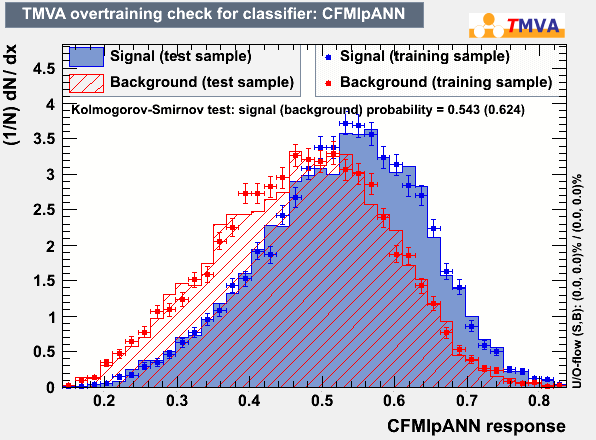
\includegraphics[width=0.45\textwidth]{Figures/Analysis_1_Diagrams/overtrain_CFMlpANN_6ormorej2t.png}
   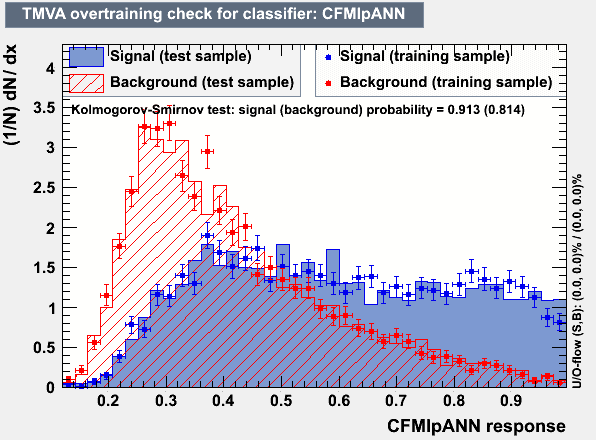
\includegraphics[width=0.45\textwidth]{Figures/Analysis_1_Diagrams/overtrain_CFMlpANN_4j3t.png}
   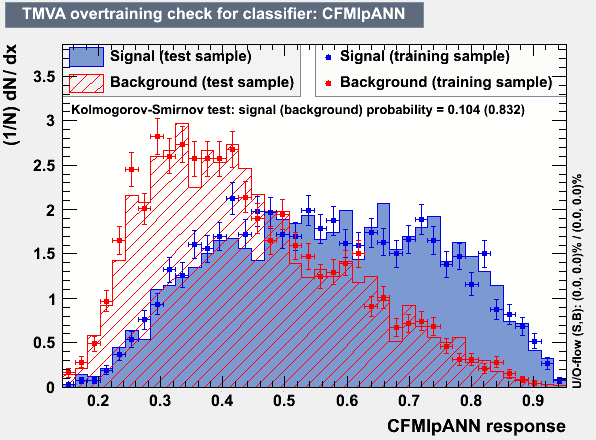
\includegraphics[width=0.45\textwidth]{Figures/Analysis_1_Diagrams/overtrain_CFMlpANN_5j3t.png}
   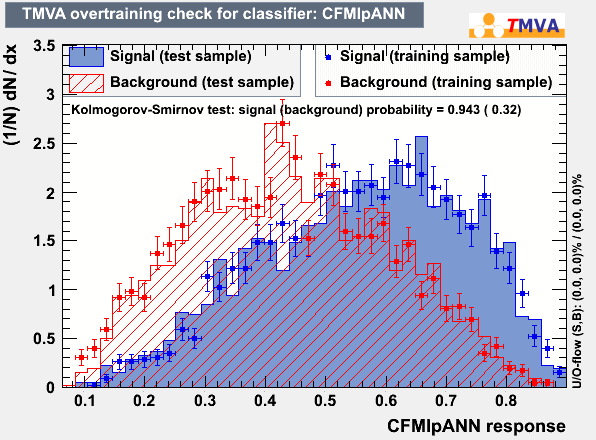
\includegraphics[width=0.45\textwidth]{Figures/Analysis_1_Diagrams/overtrain_CFMlpANN_6ormorej3t.png}
   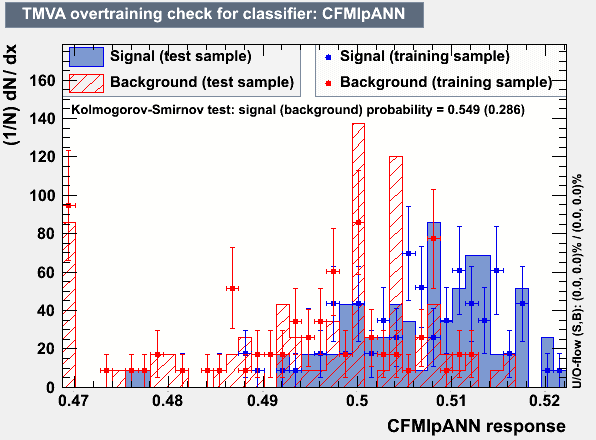
\includegraphics[width=0.45\textwidth]{Figures/Analysis_1_Diagrams/overtrain_CFMlpANN_4j4t.png}
   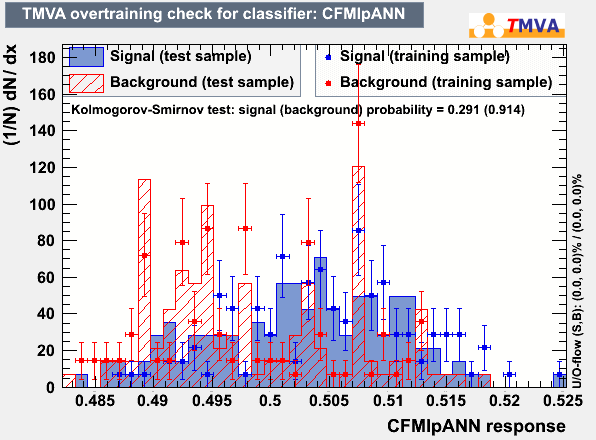
\includegraphics[width=0.45\textwidth]{Figures/Analysis_1_Diagrams/overtrain_CFMlpANN_5j4ormoret.png}
   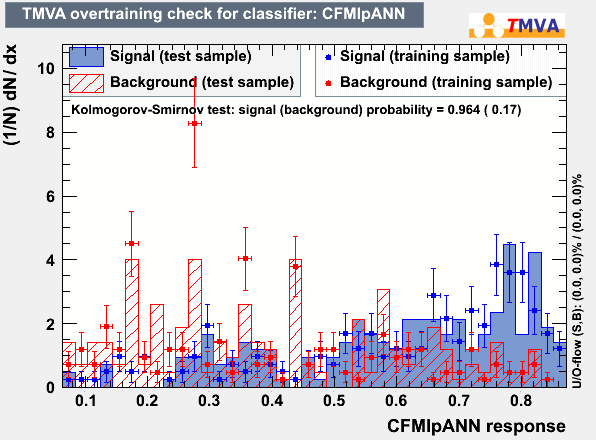
\includegraphics[width=0.45\textwidth]{Figures/Analysis_1_Diagrams/overtrain_CFMlpANN_6ormorej4ormoret.png}
      \caption{Comparisons of the testing and training samples used to
      optimize the CFMlpANN weights for each jet/tag category}
   \label{fig:ann_testTrain}
 \end{center}
\end{figure}

\par It is possible to bias the CFMlpANN response, by overtraining
it.  This is the case where the weights are over-adjusted to correctly
classify events in the training sample.  If overtrained, small
fluctuations in the input variable distributions of authentic signal
events can lead to incorrect classification of the signal events when
the CFMlpANN attempts to classify the data.  To avoid this, half of
the simulated events for \ttH signal and \ttjets background are used
during training.  After training, the other half are used to trest the
response of the algorithm.  If properly trained, the testing and
training samples should have identical CFMlpANN responses.  The figure
of merit used to assess this is the Kolomogrov-Smirnoff test, which
computes the probability that two distributions have been sampled from
the same underlying probability distribution.  The results of the
training and testing for each of the jet/tag cateories is shown in
figure \ref{fig:ann_testTrain}.  No signs of overtraining are observed.


\subsection{MVA Input Variables, Data to Monte Carlo Comparisons}
\label{mva_input_vars_data_to_mc_overview}

\par As mentioned in the previous section, each jet/tag category has
been trained with its own CFMlpANN.  Each category uses ten input
variables, except for the $\ge$6j, $\ge$4t category, which uses
eleven.  A total of 24 unique input variables are used in the 7
different jet/tag categories and are listed in
table~\ref{tab:inputs}.  The most discriminating variable for each
category is denoted by a $\bigstar$.  The inputs are selected from a
ranked list based on initial separation between signal and background.
The separation of the individual variables is evaluated using a
separation benchmark $\langle S^2 \rangle$~\cite{Hocker:2007ht}
defined as follows: 

\begin{equation} \langle S^2 \rangle = \frac{1}{2}
 \int{\frac{\left(\hat{y}_S(y) - \hat{y}_B(y)\right)^2}{\hat{y}_S(y) +
 \hat{y}_B(y)} dy}, 
\end{equation} 

\noindent where $y$ is the input variable, and $\hat{y}_S$ and
$\hat{y}_B$ are the signal and background probability density
functions for that input variable in the signal and background
samples, respectively. The maximum number of input variables
used in each category is limited by the statistics in the simulated
samples used for the CFMlpANN training. The number of variables per category is
determined by reducing the number of variables until the minimum
number of variables needed to maintain roughly the same ANN
performance is reached. In this case, 10 input variables yields stable
and approximately identical performance to using 15, while using 5
variables degraded discrimination power significantly.

\begin{table}[htp]
%\begin{adjustwidth}{-1.7in}{-1.7in}                                                                                                                                       
        
  \centering
  \noindent
  \small
    \caption{The ANN inputs for the nine jet-tag categories in the $8 \TeV$ \ttH analysis in the lepton+jets and dilepton channels. The choice of inputs
is optimized for each category. Definitions of the variables are given
in the text. The best input variable for each jet-tag category is denoted by 
$\bigstar$.}
    \label{tab:inputs}
    \begin{tabular}{|l|c|c|c|c|c|c|c||c|c|} \hline
& \multicolumn{7}{c|}{Lepton+Jets} \\ \hline
Jets& $\geq$6 & 4 & 5 & $\geq$6 & 4 & 5 & $\geq$6 \\
Tags & 2 & 3 & 3 & 3 & 4 & $\geq$4 & $\geq$4 \\ \hline \hline
Jet 1 $\pt$ & & $\checkmark$ & $\checkmark$ & & $\checkmark$ & & \\
Jet 2 $\pt$ & & $\checkmark$ & $\checkmark$ & & & &  \\
Jet 3 $\pt$ & $\checkmark$ & $\checkmark$ & $\checkmark$ & & & $\checkmark$ &   \\
Jet 4 $\pt$ & $\checkmark$ & $\checkmark$ & $\checkmark$ & & & $\checkmark$ &  \\
$\pt(\ell,\MET,\text{jets})$ & & $\bigstar$ & $\checkmark$ & & $\checkmark$ & $\checkmark$ & \\
$M(\ell,\MET,\text{jets})$ & $\checkmark$ & $\checkmark$ & & $\checkmark$ & $\checkmark$ & & $\checkmark$  \\
Average $M((\text{j}_m^{\text{untag}},\text{j}_n^{\text{untag}}))$ & $\checkmark$ & & & $\checkmark$ & & &  \\
$M((\text{j}_m^{\text{tag}},\text{j}_n^{\text{tag}})_{\text{closest}})$ & & & & & & & $\checkmark$  \\
$M((\text{j}_m^{\text{tag}},\text{j}_n^{\text{tag}})_{\text{best}})$ & & & & & & & $\checkmark$  \\
Average $\Delta R(\text{j}_m^{\text{tag}},\text{j}_n^{\text{tag}})$ & & & & $\checkmark$ & $\checkmark$ & $\checkmark$ & $\checkmark$  \\
Minimum $\Delta R(\text{j}_m^{\text{tag}},\text{j}_n^{\text{tag}})$ & & & $\checkmark$ & & & & \\
$\Delta R(\ell,\text{j}_{\text{closest}})$ & & & & & & $\checkmark$ & $\checkmark$ \\
Sphericity & $\checkmark$ & & & $\checkmark$ & & & $\checkmark$ \\
Aplanarity & $\checkmark$ & & & & $\checkmark$ & &  \\
$H_0$ & $\checkmark$ & & & & & &   \\
$H_1$ & $\checkmark$ & & & & $\checkmark$ & & \\
$H_2$ & & & & $\checkmark$ & & & $\checkmark$    \\
$H_3$ & $\bigstar$ & & & $\checkmark$ & & & $\checkmark$  \\
$\mu^{\text{CSV}}$ & $\checkmark$ & $\checkmark$ & $\bigstar$ & $\bigstar$ & $\bigstar$ & $\bigstar$ & $\bigstar$  \\
$(\sigma_n^{\text{CSV}})^2$ & & $\checkmark$ & $\checkmark$ & $\checkmark$ & $\checkmark$ & $\checkmark$ &  \\
Highest CSV value & & & & & & $\checkmark$ &  \\
2$^{nd}$-highest CSV value & & $\checkmark$ & $\checkmark$ & $\checkmark$ & $\checkmark$ & $\checkmark$ & $\checkmark$  \\
Lowest CSV value & & $\checkmark$ & $\checkmark$ & $\checkmark$ & $\checkmark$ & $\checkmark$ & $\checkmark$ \\ \hline
 \end{tabular}
\end{table}

\par The input variables used in the CFMlpANN can be broken down into
several classes.  The first is related to jet, and multi-object
kinematics.  The $b$-jets produced by the Higgs boson tend to have a
harder $p_{T}$ spectrum compared to $b$-jets produced from gluon
radiation.  Additionally, the recoil of the Higgs off of the
top-system produces small differences in the $p_{T}$ and invariant
mass of the recosntructed \ttjets system. 

\begin{itemize}
  \item Jet 1 $\pt$ - the highest value of transverse jet momentum in
    the event
  \item Jet 2 $\pt$ - the second highest value of transverse jet
    momentum in the event
  \item Jet 3 $\pt$  - the third highest value of transverse jet
    momentum in the event
  \item Jet 4 $\pt$  - the fourth highest value of transverse jet
    momentum in the event
  \item $\pt(\ell,\MET,\text{jets})$ - the transverse momentum of the
    four-vector formed by summing the four-vectors of the lepton, MET,
    and all selected jets in the event
  \item $M(\ell,\MET,\text{jets})$ - the invariant mass of the
    four-vector formed by summing the four-vectors of the lepton, MET<
    and all selected jets in the event
  \item Average
    $M((\text{j}_m^{\text{untag}},\text{j}_n^{\text{untag}}))$ - the
    average di-Jet mass formed by all combinations of jets that have
    not been $b$-tagged in the event
  \item
    $M((\text{j}_m^{\text{tag}},\text{j}_n^{\text{tag}})_{\text{closest}})$
    - the invariant di-Jet mass of the two $b$-tagged jets that are
    closest to one another in the detector
  \item
    $M((\text{j}_m^{\text{tag}},\text{j}_n^{\text{tag}})_{\text{best}})$
    - the invariant mass constructed from the two tagged jets least
    likely to be a part of the $\ttbar$ system as determined by a
    minimum $\chi^2$ search among all the jet, lepton, and $\MET$
    combinations in the event, using the $W$ boson and top masses as
    kinematic constraints.
\end{itemize}

\par The next class of input variables describe the angular
relationship between reconstructed objects in the event.  These are
event shape variables.  Production of a relatively massive object, in
addition to top quarks, such as the Higgs, tends to make $\ttH$
events more spherically distributed in the detected, while the
background events are more collimated.  Variables in this class
include angular correlations, like the opening angle between the
tagged jets 

\begin{itemize}
  \item Average $\Delta
    R(\text{j}_m^{\text{tag}},\text{j}_n^{\text{tag}})$  - the average
    $\Delta$R spatial separation between all cominations of $b$-tagged
    jets in the event
  \item Minimum $\Delta
    R(\text{j}_m^{\text{tag}},\text{j}_n^{\text{tag}})$ - the smallest
    value of $\Delta$R measured between a pair of $b$-tagged jets
  \item $\Delta R(\ell,\text{j}_{\text{closest}})$ - the $\Delta$R
    spatial separation of the lepton and the closest reconstructed jet
  \item Sphericity - Event shape variable equal to $\frac{3}{2}
    (\lambda_{2} + \lambda_{3})$, where $\lambda_{2}$ and
    $\lambda_{3}$ are the second and third eigenvalues of the
    sphericity tensor as described in\cite{sphericity} 
  \item Aplanarity - Event shape variable equal to
    \(\frac{3}{2}(\lambda_{3})\), where \(\lambda_{3}\) is the third
    eigenvalue of the sphericity tensor as described in 
  \item $H_0$ - the zeroth Fox-Wolfram moment ~\cite{FoxWolfram}
  \item $H_1$ - the first Fox-Wolfram moment 
  \item $H_2$ - the second Fox-Wolfram moment
  \item $H_3$ - the third Fox-Wolfram moment
\end{itemize}

\noindent where $\Delta R = \sqrt{\Delta\eta^{2} + \Delta\phi^{2}}$.
The sphericity tensor is given by the equation:

\begin{equation}\label{eq:sphericity_tensor}
S^{a,b} = \frac{ \sum_{i}p_{i}^{a}p_{i}^{b} }{ \sum_{i} |\hat{p_{i}}|^{2} }
\end{equation}

\noindent where $a,b = x,y,z$ coordinates.  This tensor is
diagonalized, and solved for its eigenvalues, which are used to
compute the sphericity and aplanarity variables.  The Fox-Wolfram
moments are defined are momentum weighted spherical harmonics, defined
as: 

\begin{equation}\label{eq:fox_wolfram}
H_{\ell} = \sum_{i,j=1}^{N_{Jets}} \frac{ |\hat{p_{i}}||\hat{p_{j}}|
}{ |\hat{p}|_{tot}^{2} } P_{\ell}(\cos{\Omega_{ij}})
\end{equation}

\noindent where $P_{\ell}(\cos{\Omega_{ij}})$ is the $\ell^{th}$
spherical harmonic, with polar angle calculated between jets i and j.  

\par The final class of variables is based on the discriminant output
from the b-tagging algorithm.  For many of the categories, the average
$b$-tag discriminant of all of the jets in the event tends to be the
most powerful single variable.  This is due to the high multiplicity
of authentic $b$-jets in a \ttH event. 

\begin{itemize}
  \item $\mu^{\text{CSV}}$ - the average value of the output of the
    CSV algorithm for all selected jets in the event.  
  \item $(\sigma_n^{\text{CSV}})^2$ - the variance of the average value of the output of the
    CSV algorithm for all selected jets in the event. 
  \item Highest CSV value - the highest value of the CSV discriminant
    for any selected jet in the event 
  \item 2$^{nd}$-highest CSV value - the second highest value of the CSV discriminant
    for any selected jet in the event 
  \item Lowest CSV value - the lowest value of the CSV discriminant
    for any selected jet in the event 
\end{itemize}

\par The modeling of the input variables is compared against data for
each of the jet/tag diagrams in the the following figures: 

\begin{itemize}
  \item $\ge$6 jets,  $==$2 $b$-tags: Figure
    \ref{fig:lj_input_6j_2t_part1}, and Figure \ref{fig:lj_input_6j_2t_part2}
  \item $==$4 jets, $==$3 $b$-tags: Figure
    \ref{fig:lj_input_4j_3t_part1}, and Figure \ref{fig:lj_input_4j_3t_part2}
  \item $==$5 jets, $==$3 $b$-tags: Figure
    \ref{fig:lj_input_5j_3t_part1}, and Figure
    \ref{fig:lj_input_5j_3t_part2}
  \item $\ge$6 jets, $==$3 $b$-tags: Figure
    \ref{fig:lj_input_6j_3t_part1}, and Figure \ref{fig:lj_input_6j_3t_part2}
  \item $==$4 jets, $==$4 $b$-tags: Figure
    \ref{fig:lj_input_4j_4t_part1}, and Figure \ref{fig:lj_input_4j_4t_part2}
  \item $==$5 jets, $==$4 $b$-tags: Figure
    \ref{fig:lj_input_5j_4t_part1}, and Figure \ref{fig:lj_input_5j_4t_part2}
  \item $\ge$6 jets, $\ge$4 $b$-tags: Figure
    \ref{fig:lj_input_6j_4t_part1}, and Figure \ref{fig:lj_input_6j_4t_part2}
\end{itemize}

\noindent Below each histogram is a ratio of the yields for data over the
simulated sample prediction.  The green band is the total uncertainty
estimated for the simulation, and the error bars on the points are
determined by the statistical error on the data collected.  


%%%%%%%%%%%%%%%%%%%%%%%%%%%%%%%%%%%%%%%%%%%%%%%%%%%%%%%%%%%%%%%
%
%  NN Inputs 6j2t L+J (muon+electron) 8TeV
%
%%%%%%%%%%%%%%%%%%%%%%%%%%%%%%%%%%%%%%%%%%%%%%%%%%%%%%%%%%%%%%%

\clearpage

\begin{figure}[hbtp]
 \begin{center}
   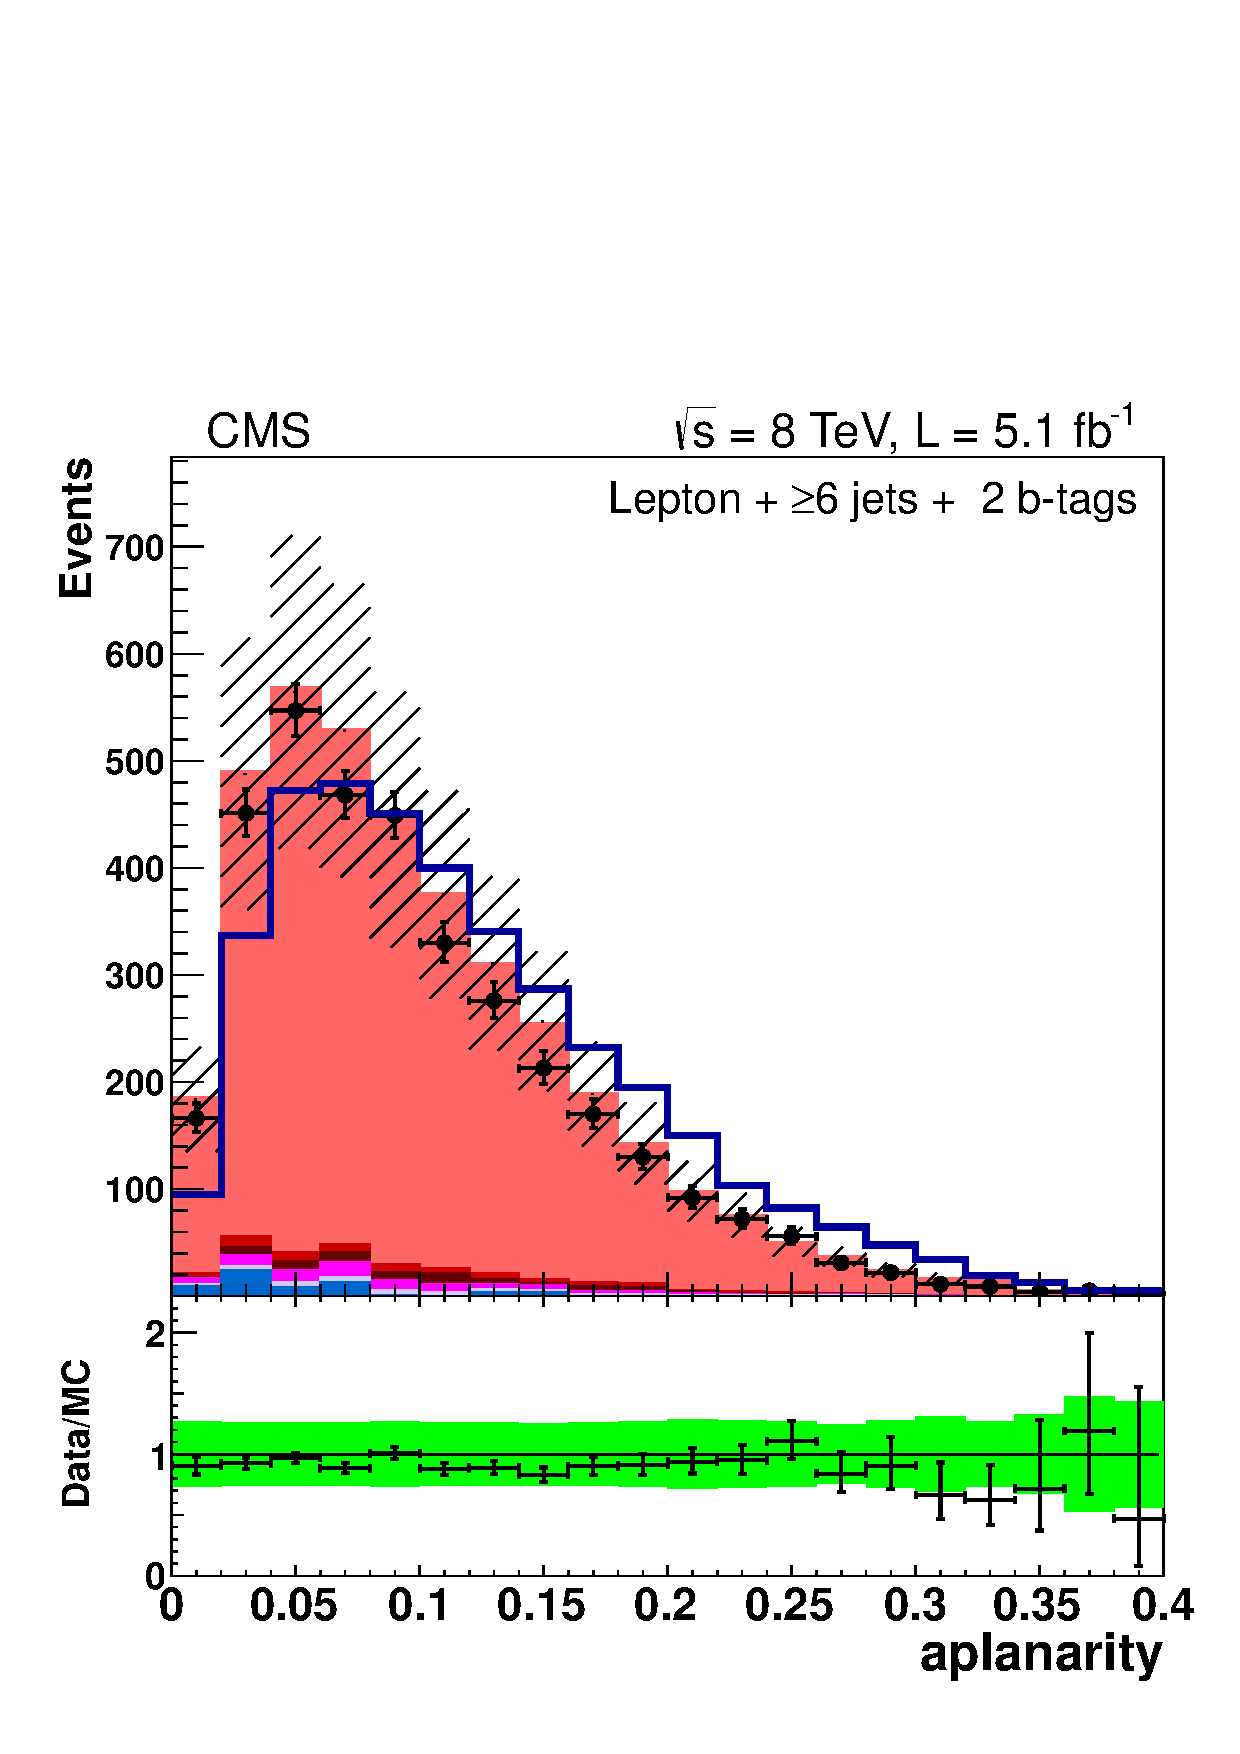
\includegraphics[width=0.31\textwidth]{Figures/Analysis_1_Diagrams/d2MCPlots_aplanarity_cut3_jge6_t2_Combined_HtWgt.pdf}
   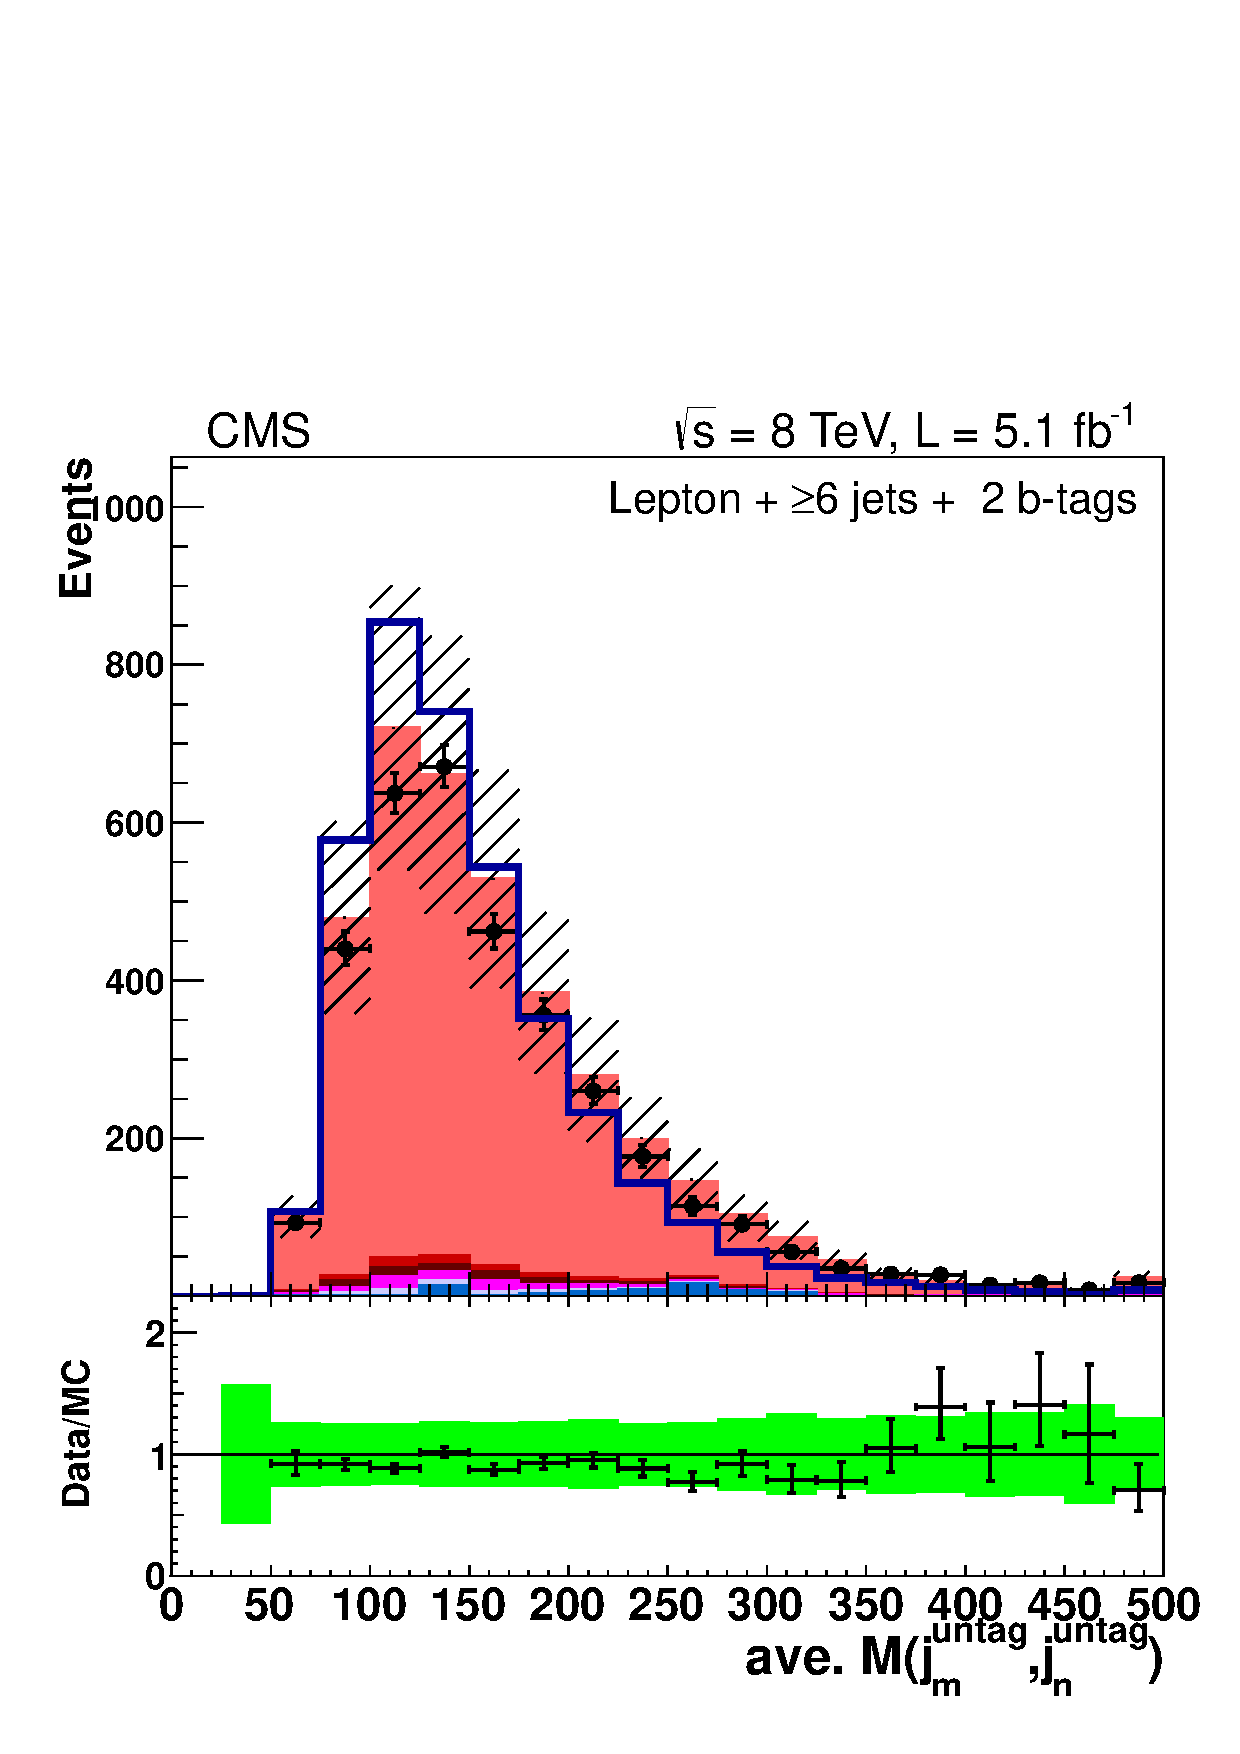
\includegraphics[width=0.31\textwidth]{Figures/Analysis_1_Diagrams/d2MCPlots_avg_untagged_dijet_mass_cut3_jge6_t2_Combined_HtWgt.pdf}
   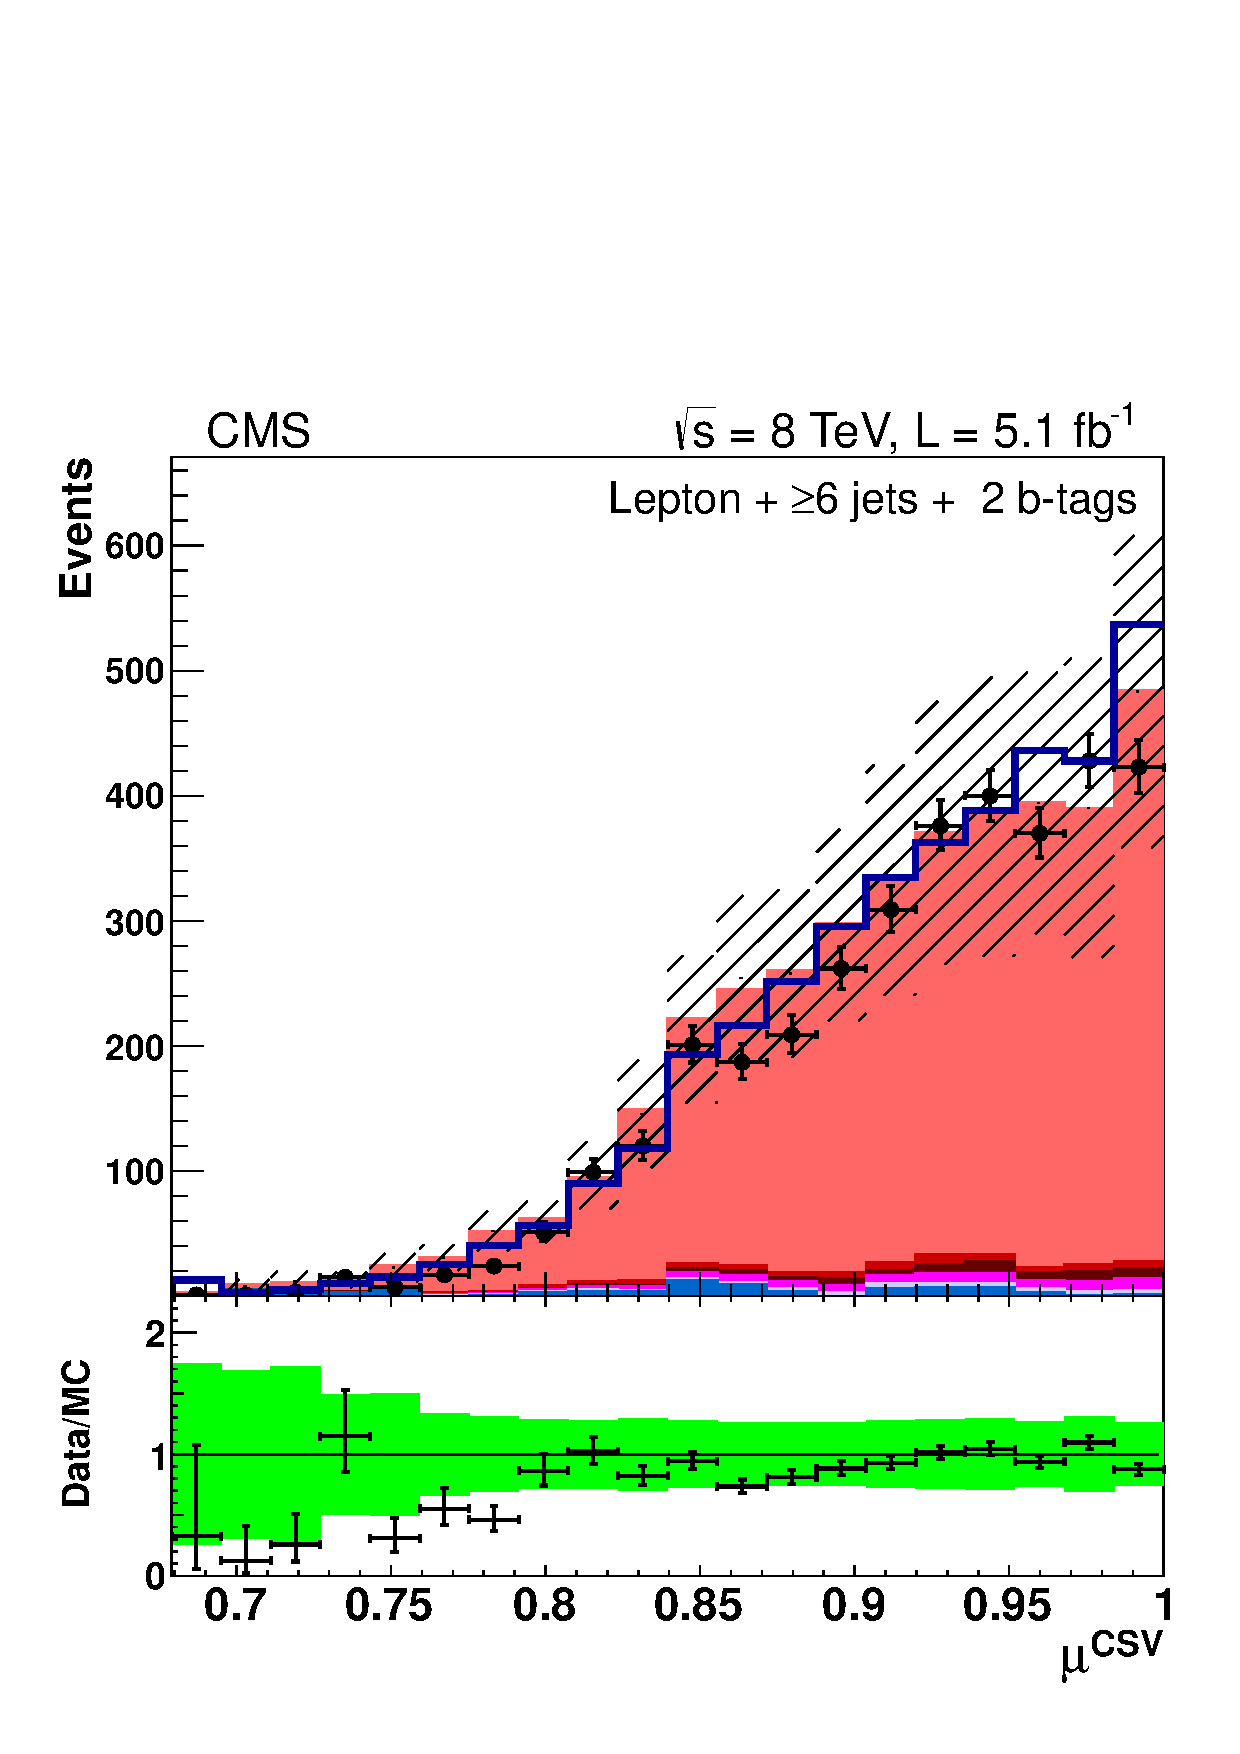
\includegraphics[width=0.31\textwidth]{Figures/Analysis_1_Diagrams/d2MCPlots_avg_btag_disc_btags_cut3_jge6_t2_Combined_HtWgt.pdf}
   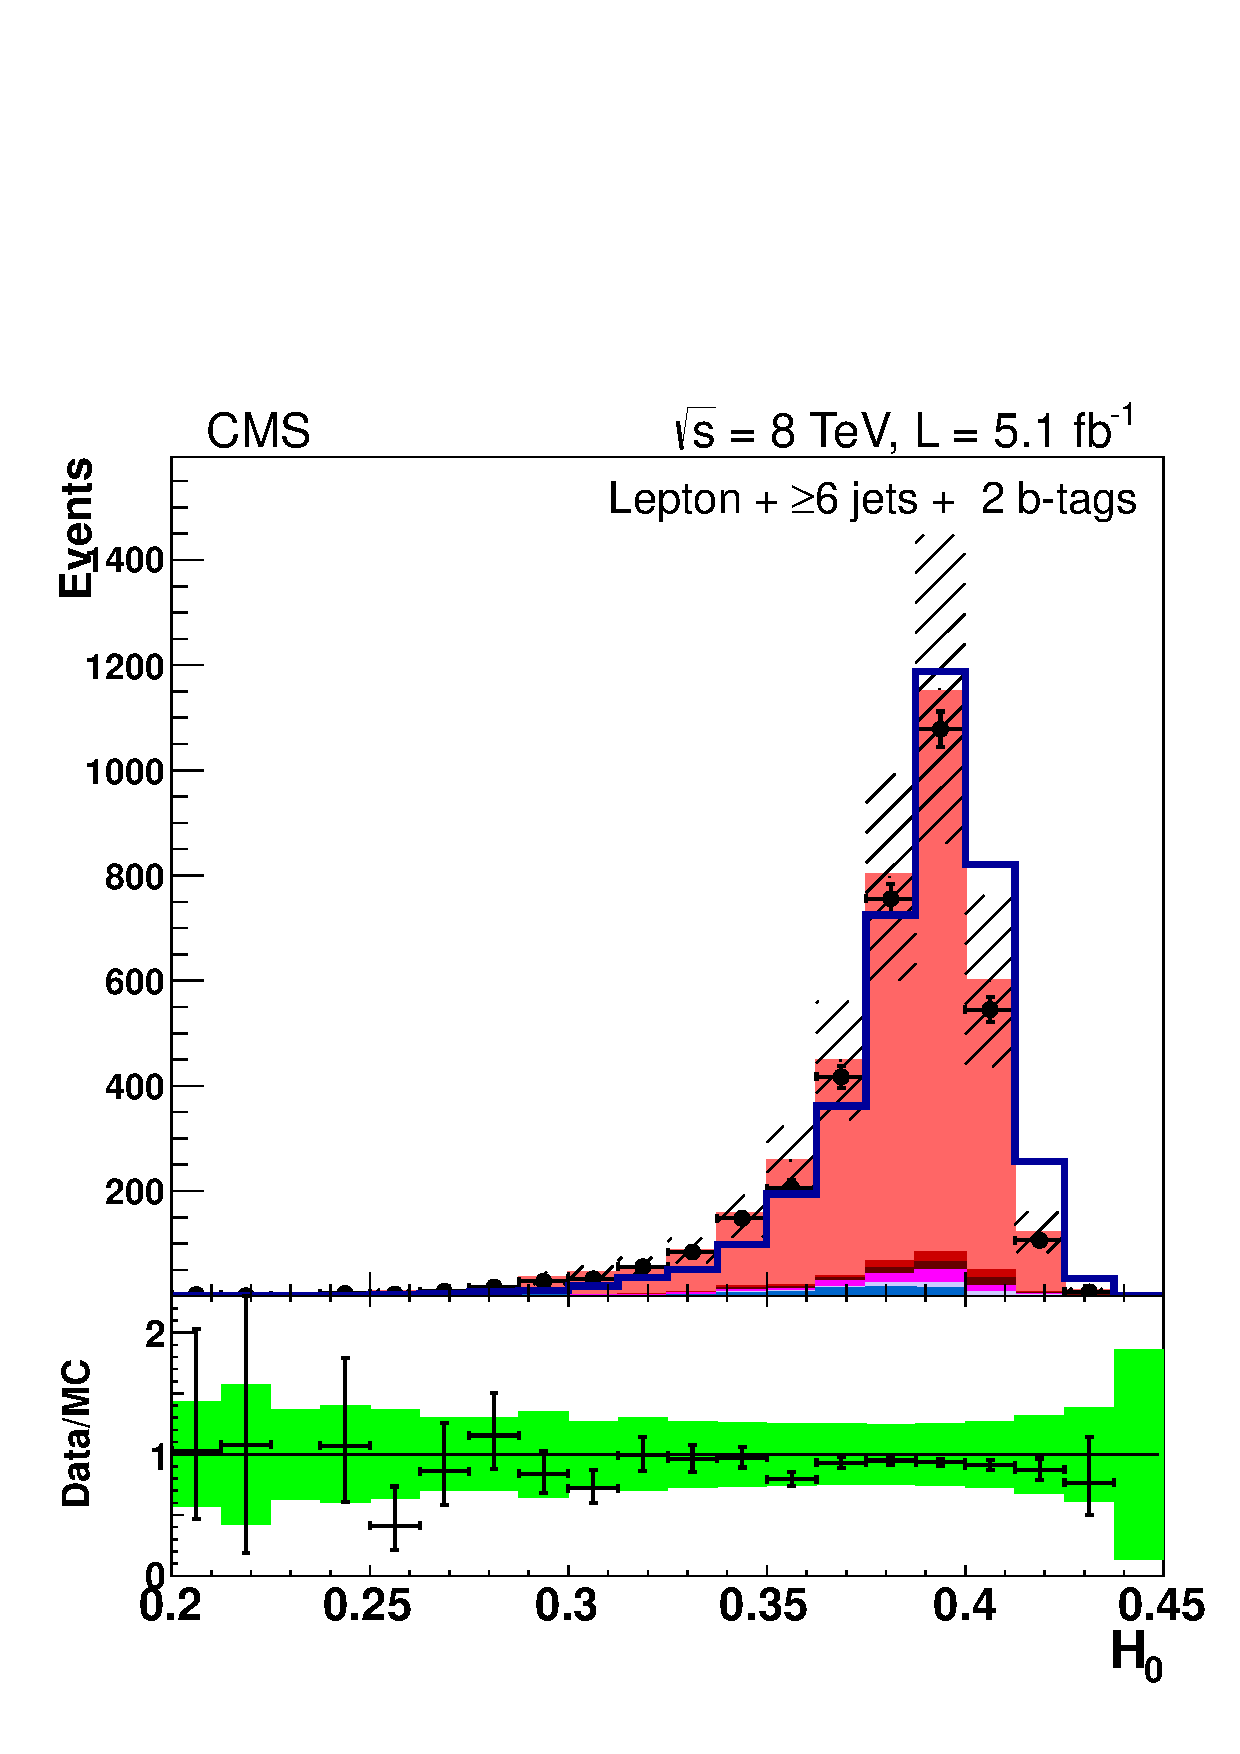
\includegraphics[width=0.31\textwidth]{Figures/Analysis_1_Diagrams/d2MCPlots_h0_cut3_jge6_t2_Combined_HtWgt.pdf}
   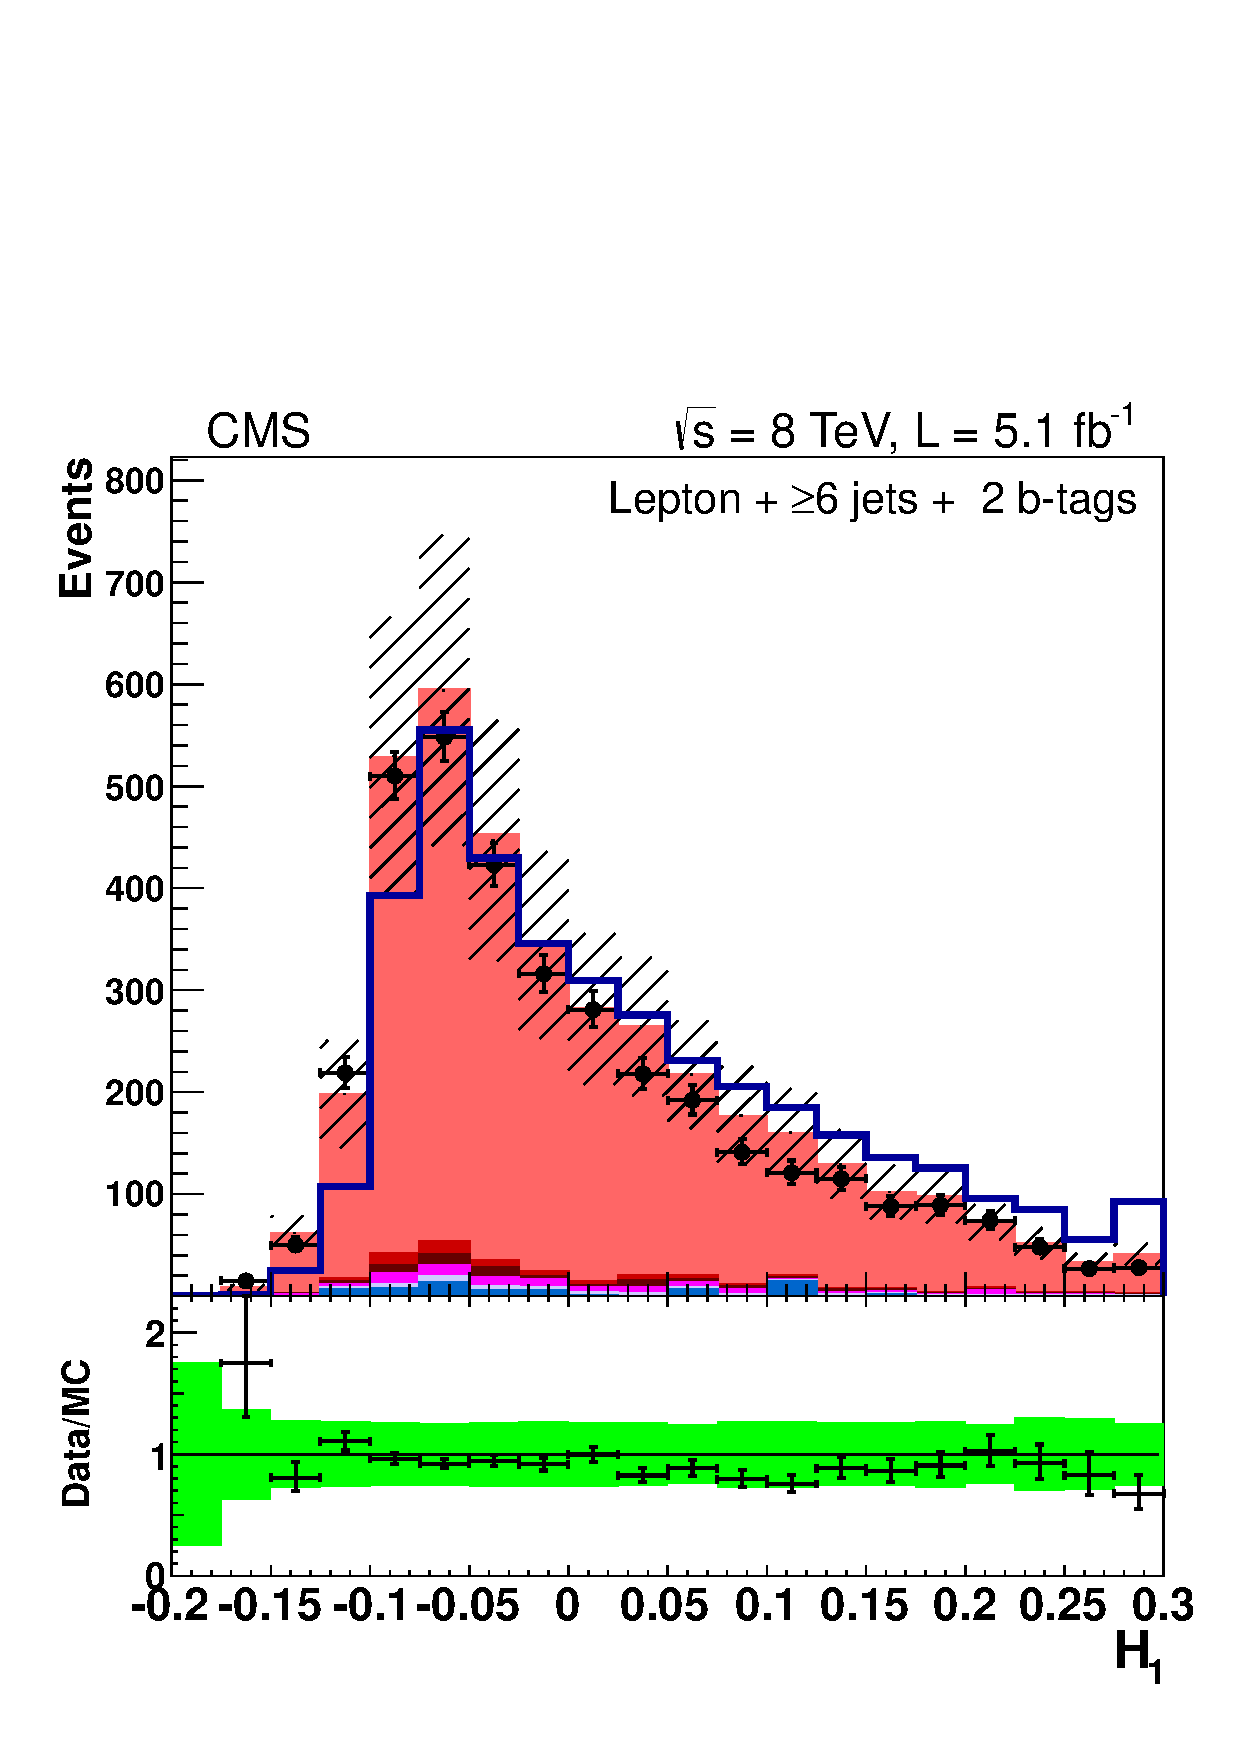
\includegraphics[width=0.31\textwidth]{Figures/Analysis_1_Diagrams/d2MCPlots_h1_cut3_jge6_t2_Combined_HtWgt.pdf}
   \raisebox{0.1\height}{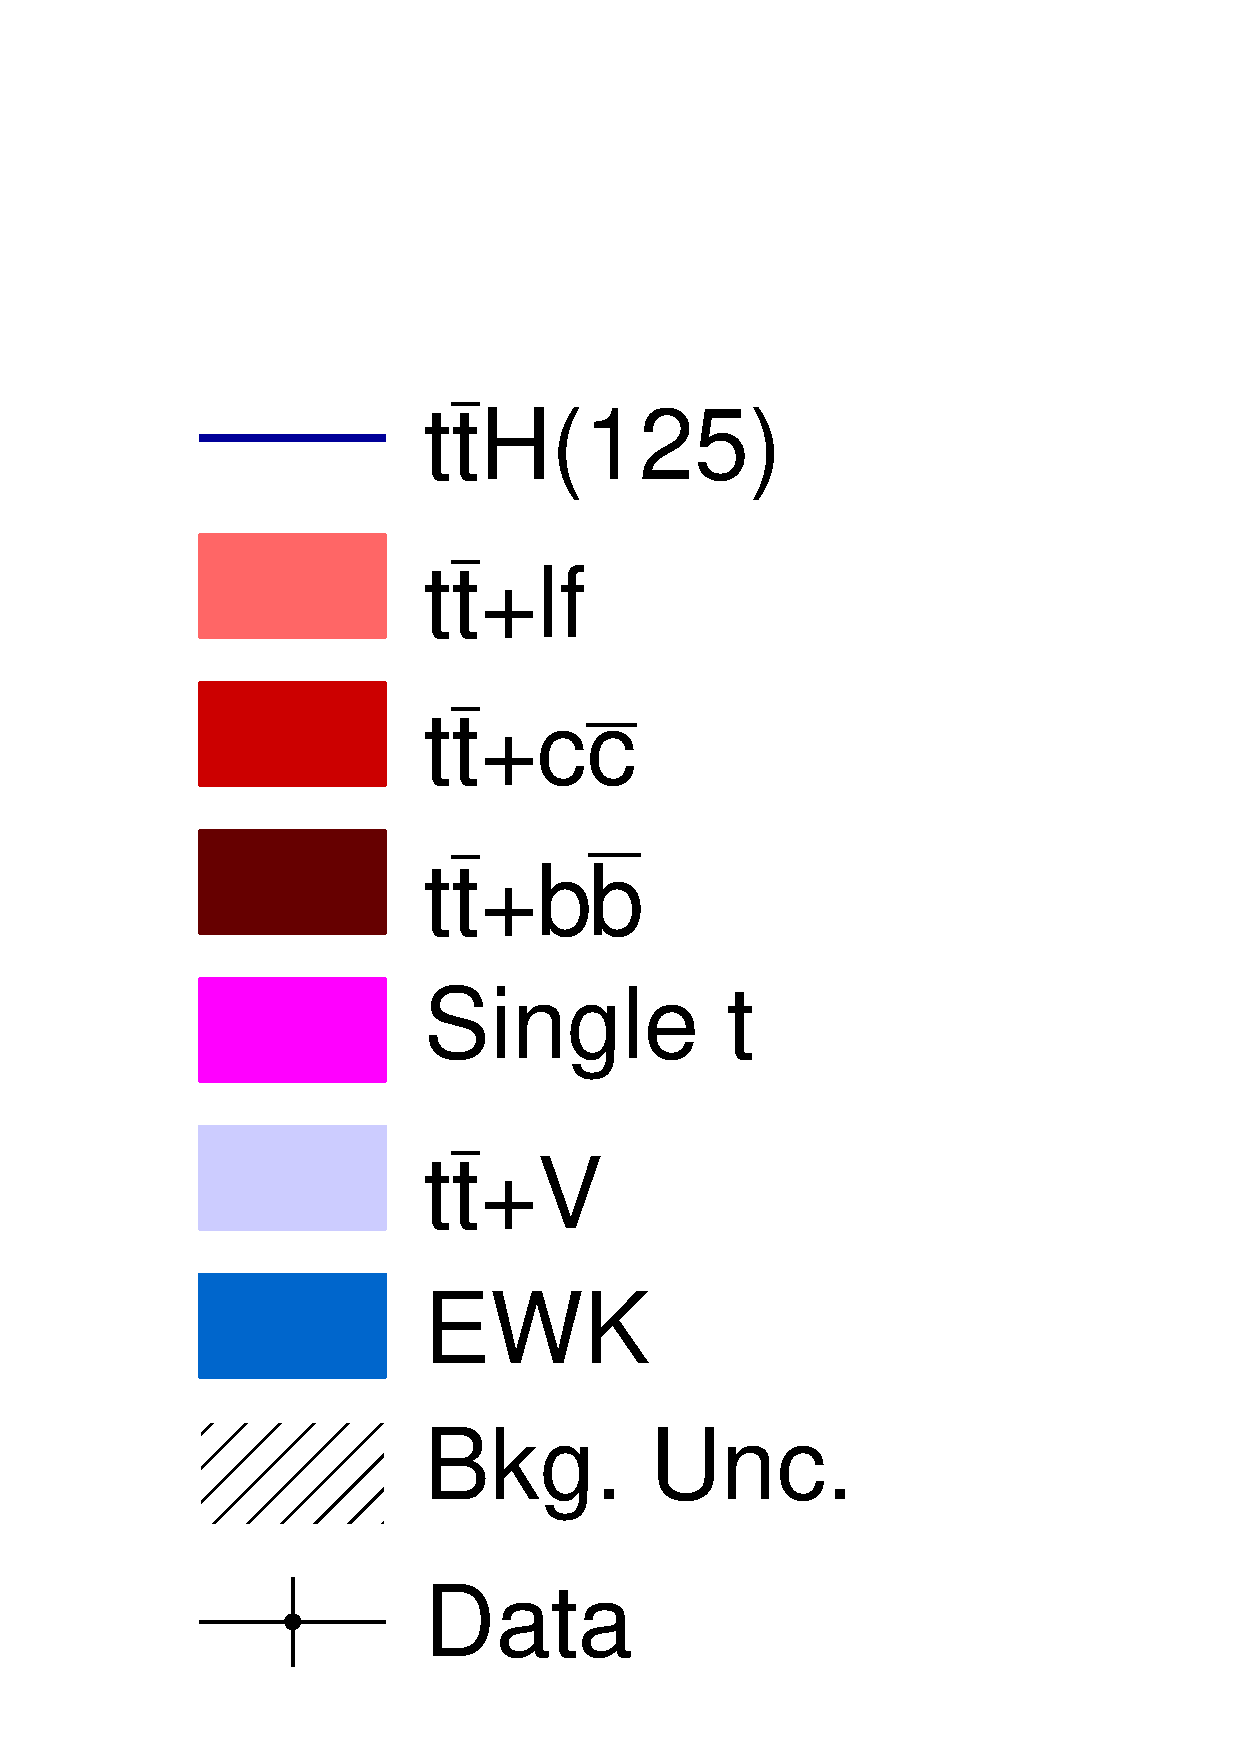
\includegraphics[width=0.25\textwidth]{Figures/Analysis_1_Diagrams/samples_legend_tall_noTTHscale.pdf}}
   \hspace{0.055\textwidth}
   \caption{Lepton + jets data/MC comparison for the $\ge$6 jets + 2 tag category.  The uncertainty band includes statistical and systematic uncertainties that affect both the rate and shape of the background distributions.}
   \label{fig:lj_input_6j_2t_part1}
   \hspace{0.055\textwidth}
 \end{center}
\end{figure}

\clearpage

\begin{figure}[hbtp]
 \begin{center}
   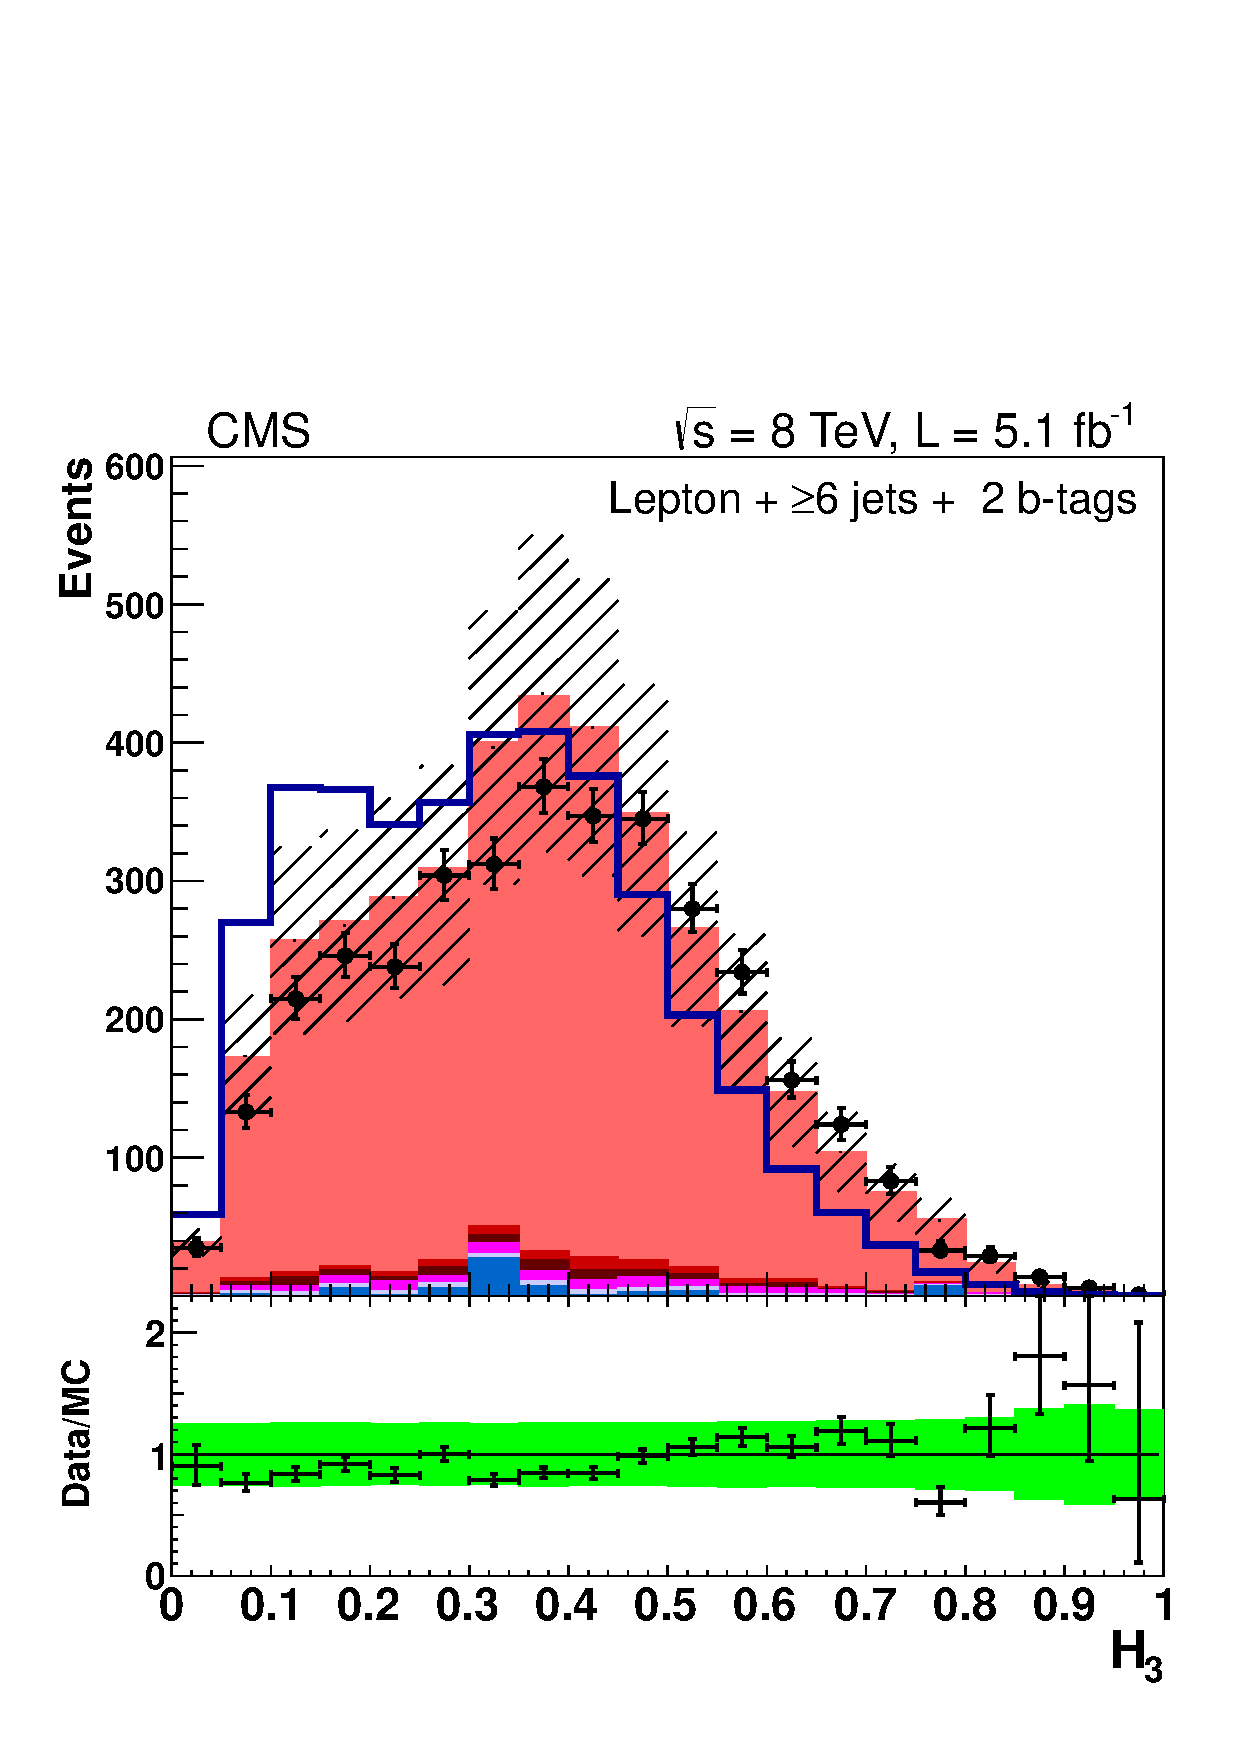
\includegraphics[width=0.31\textwidth]{Figures/Analysis_1_Diagrams/d2MCPlots_h3_cut3_jge6_t2_Combined_HtWgt.pdf}
   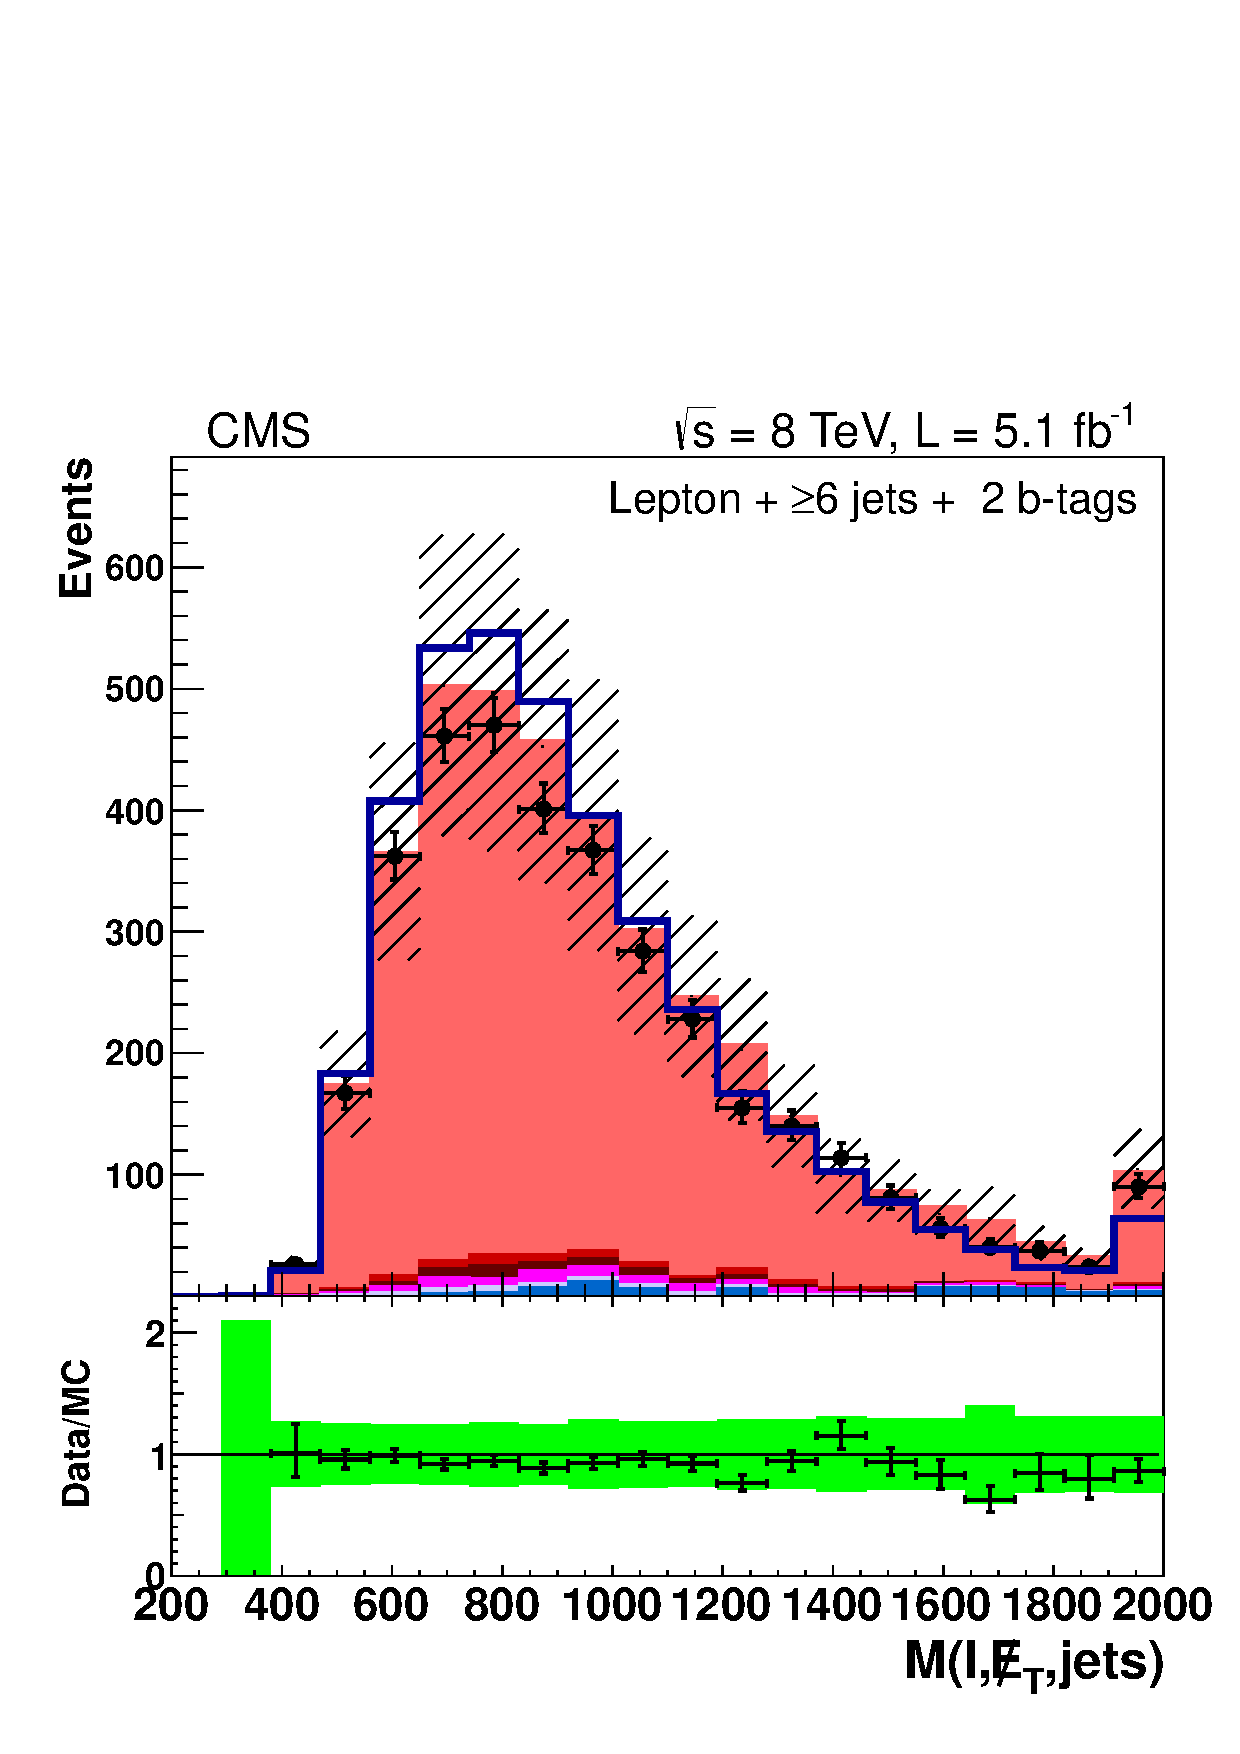
\includegraphics[width=0.31\textwidth]{Figures/Analysis_1_Diagrams/d2MCPlots_dijet_mass_of_everything_cut3_jge6_t2_Combined_HtWgt.pdf}
   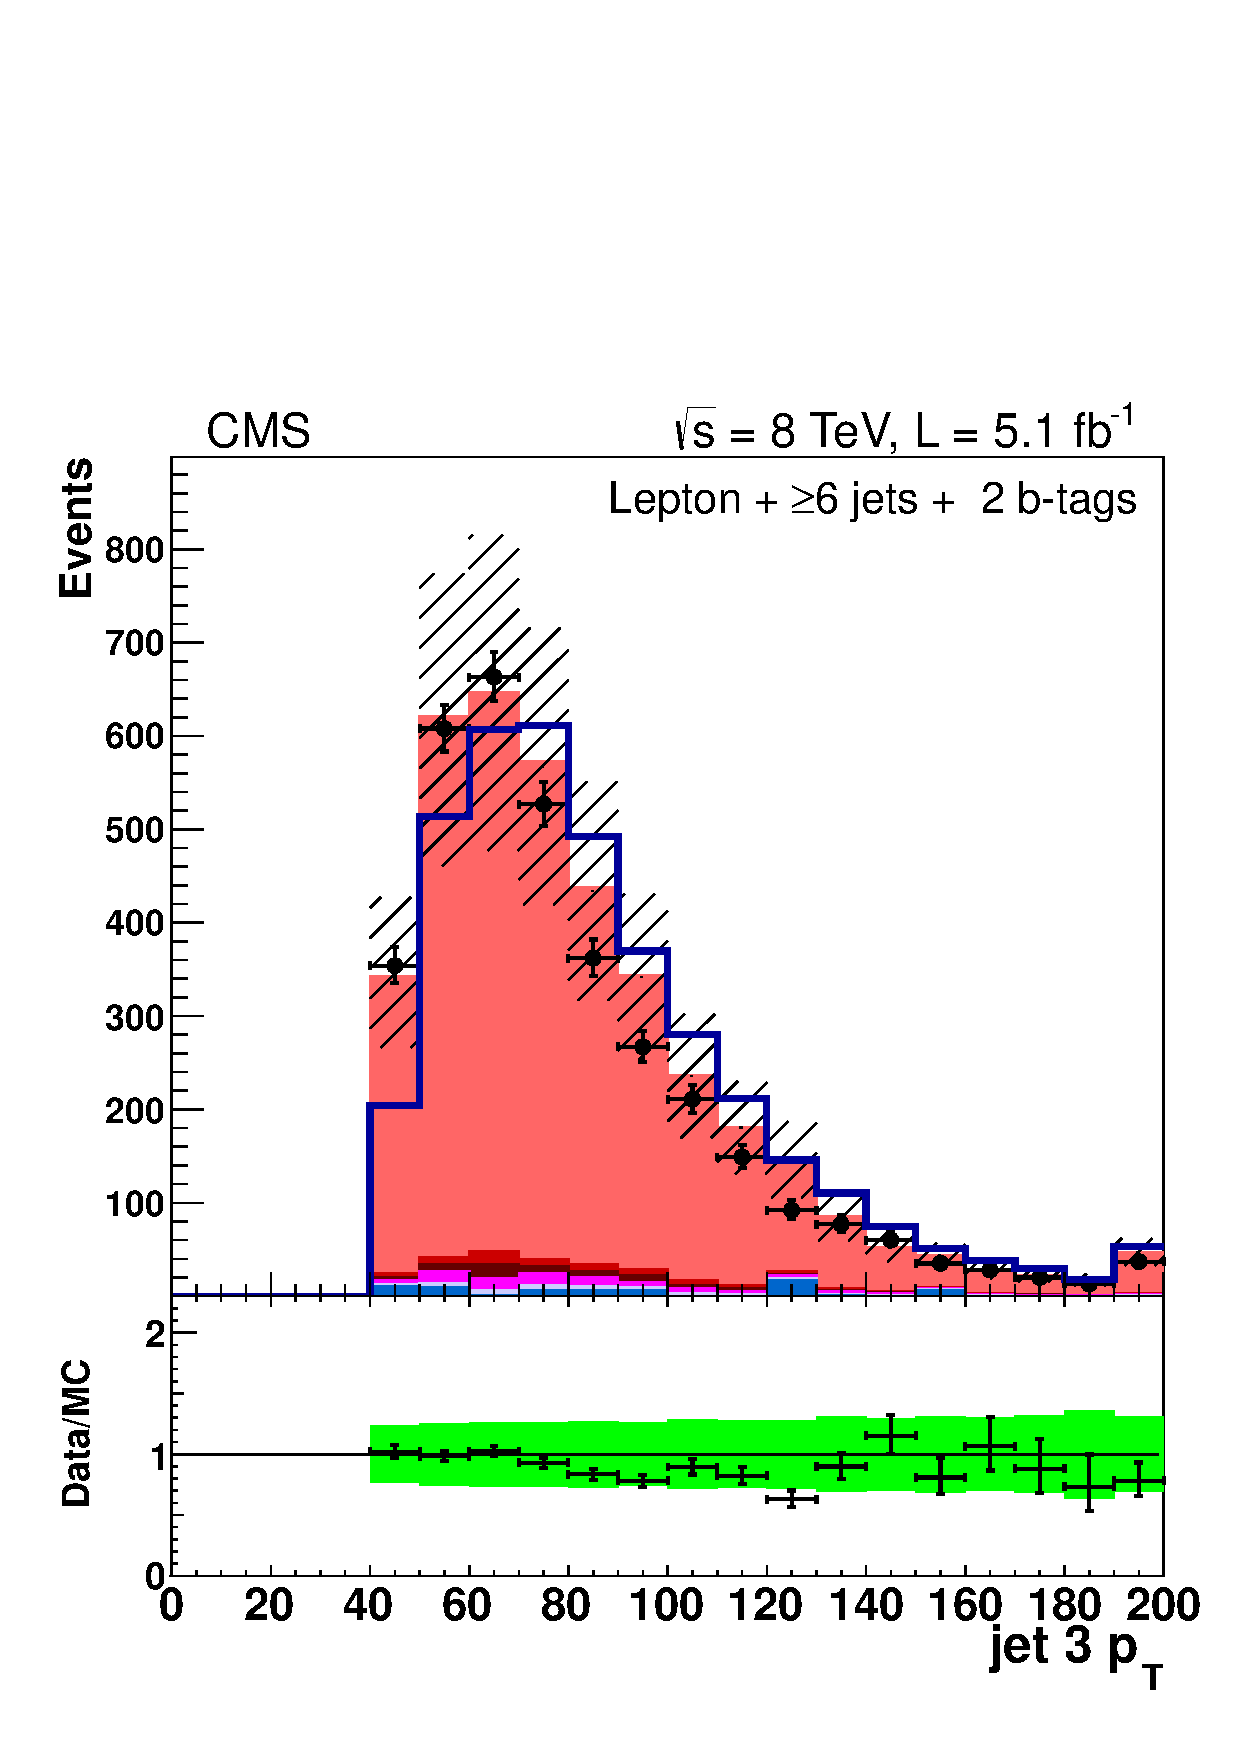
\includegraphics[width=0.31\textwidth]{Figures/Analysis_1_Diagrams/d2MCPlots_third_jet_pt_cut3_jge6_t2_Combined_HtWgt.pdf}
   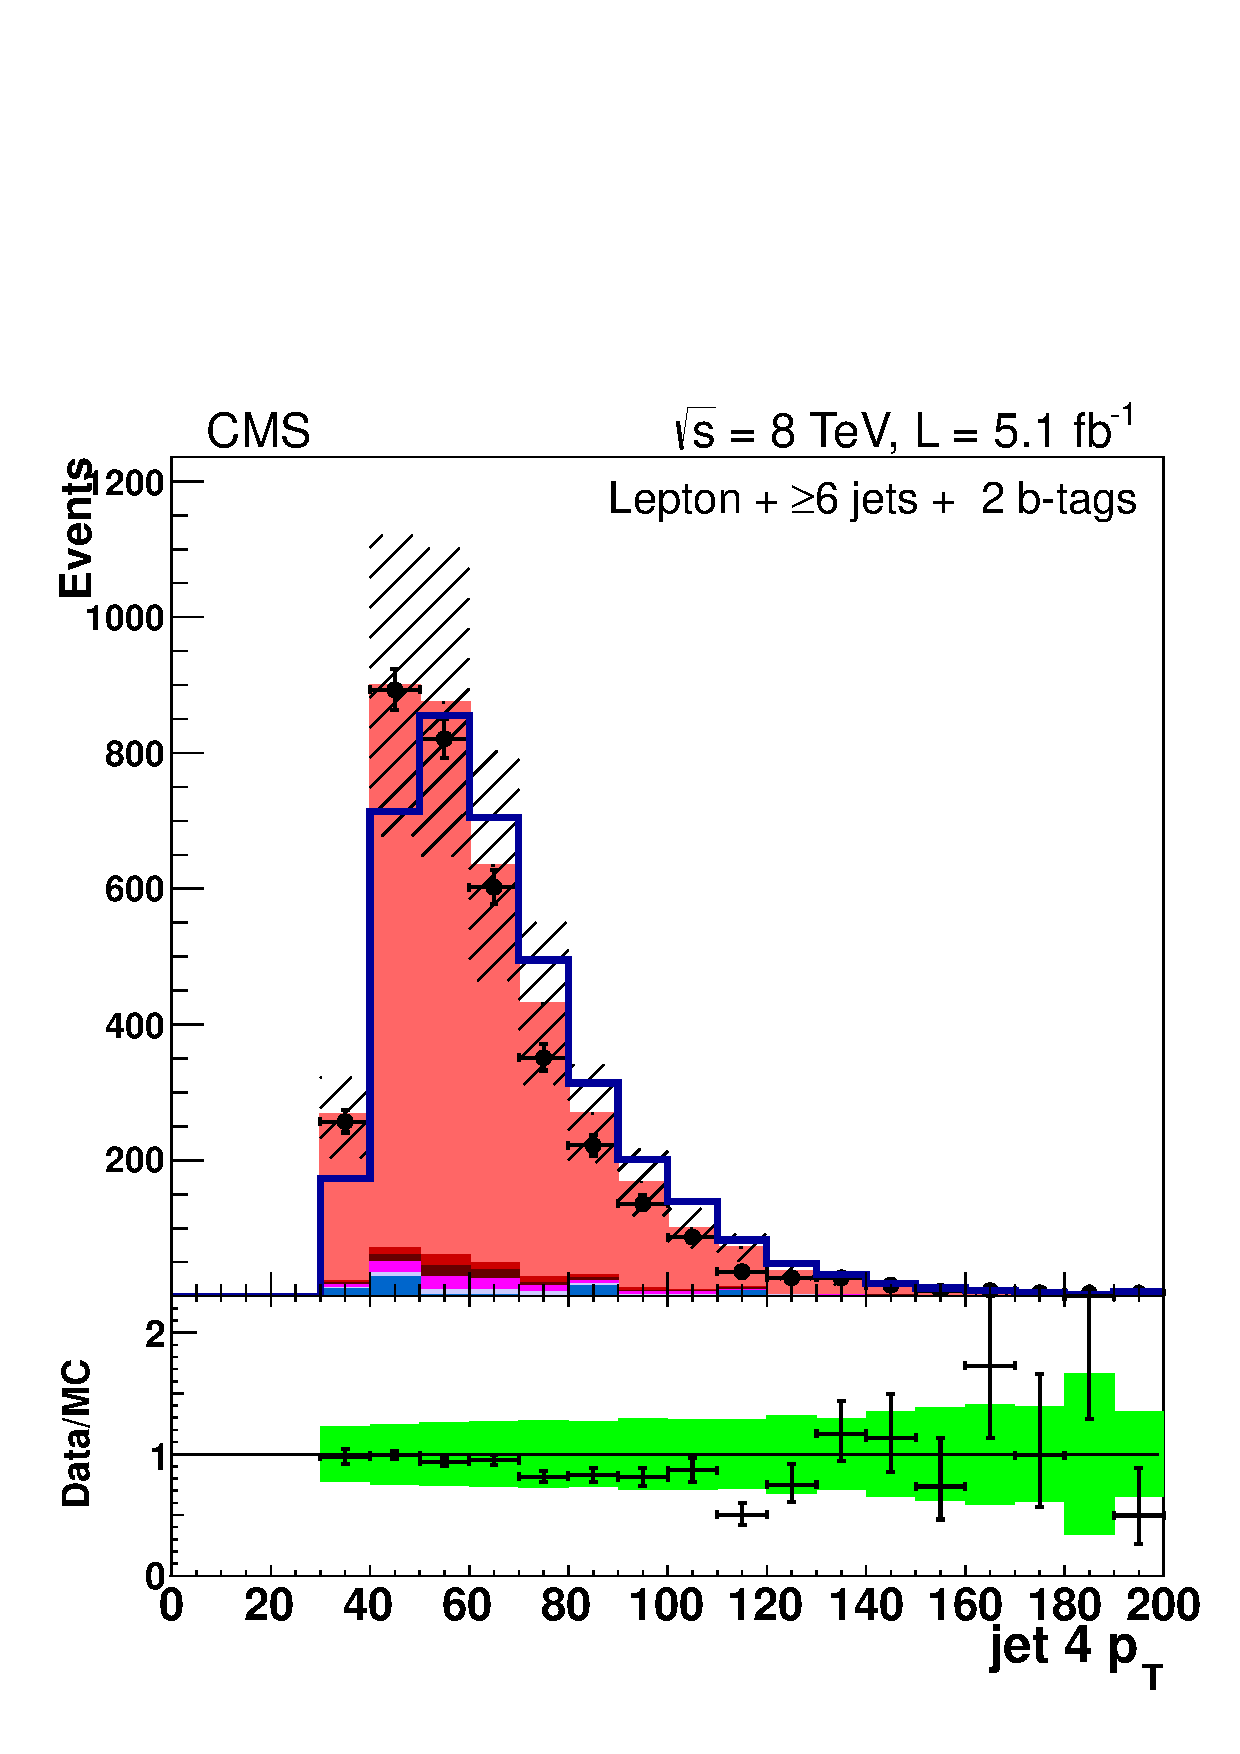
\includegraphics[width=0.31\textwidth]{Figures/Analysis_1_Diagrams/d2MCPlots_fourth_jet_pt_cut3_jge6_t2_Combined_HtWgt.pdf}
   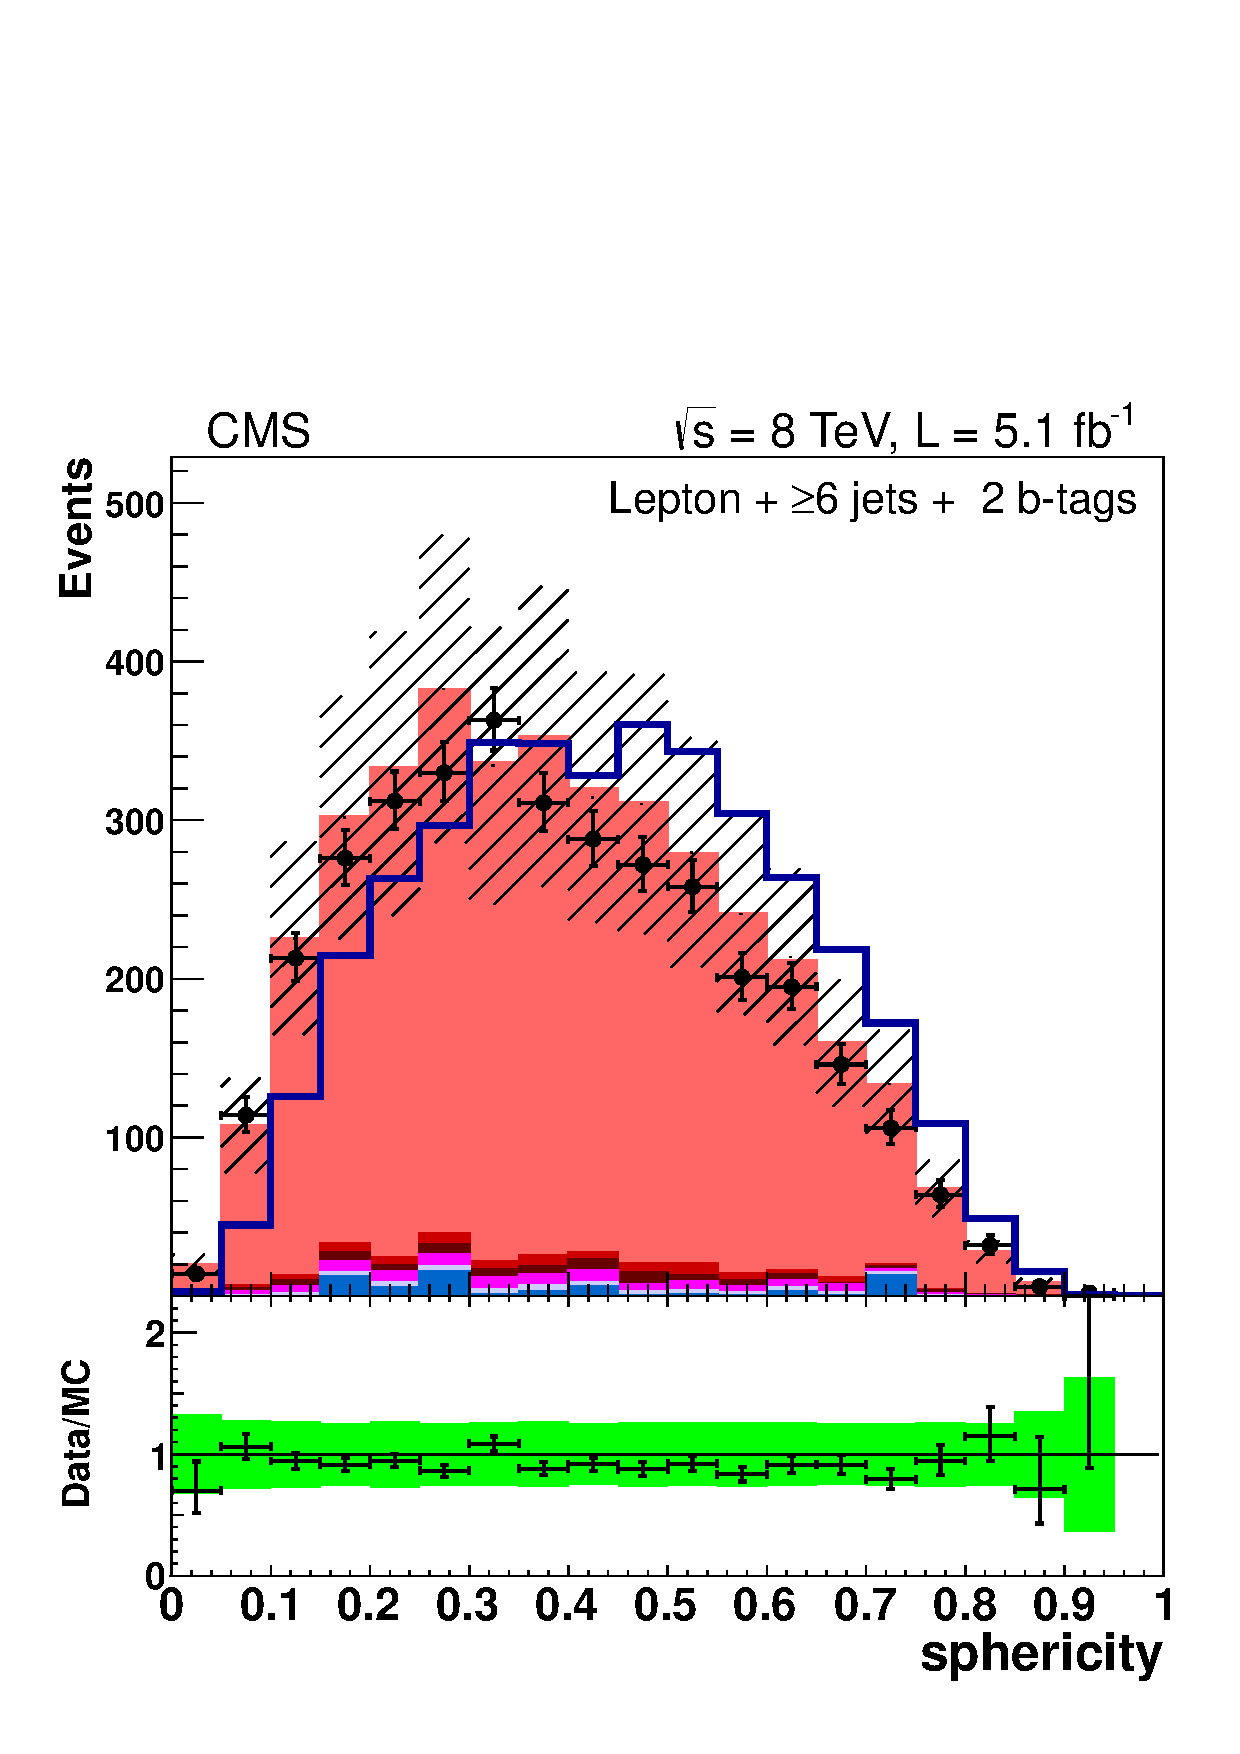
\includegraphics[width=0.31\textwidth]{Figures/Analysis_1_Diagrams/d2MCPlots_sphericity_cut3_jge6_t2_Combined_HtWgt.pdf}
   \raisebox{0.1\height}{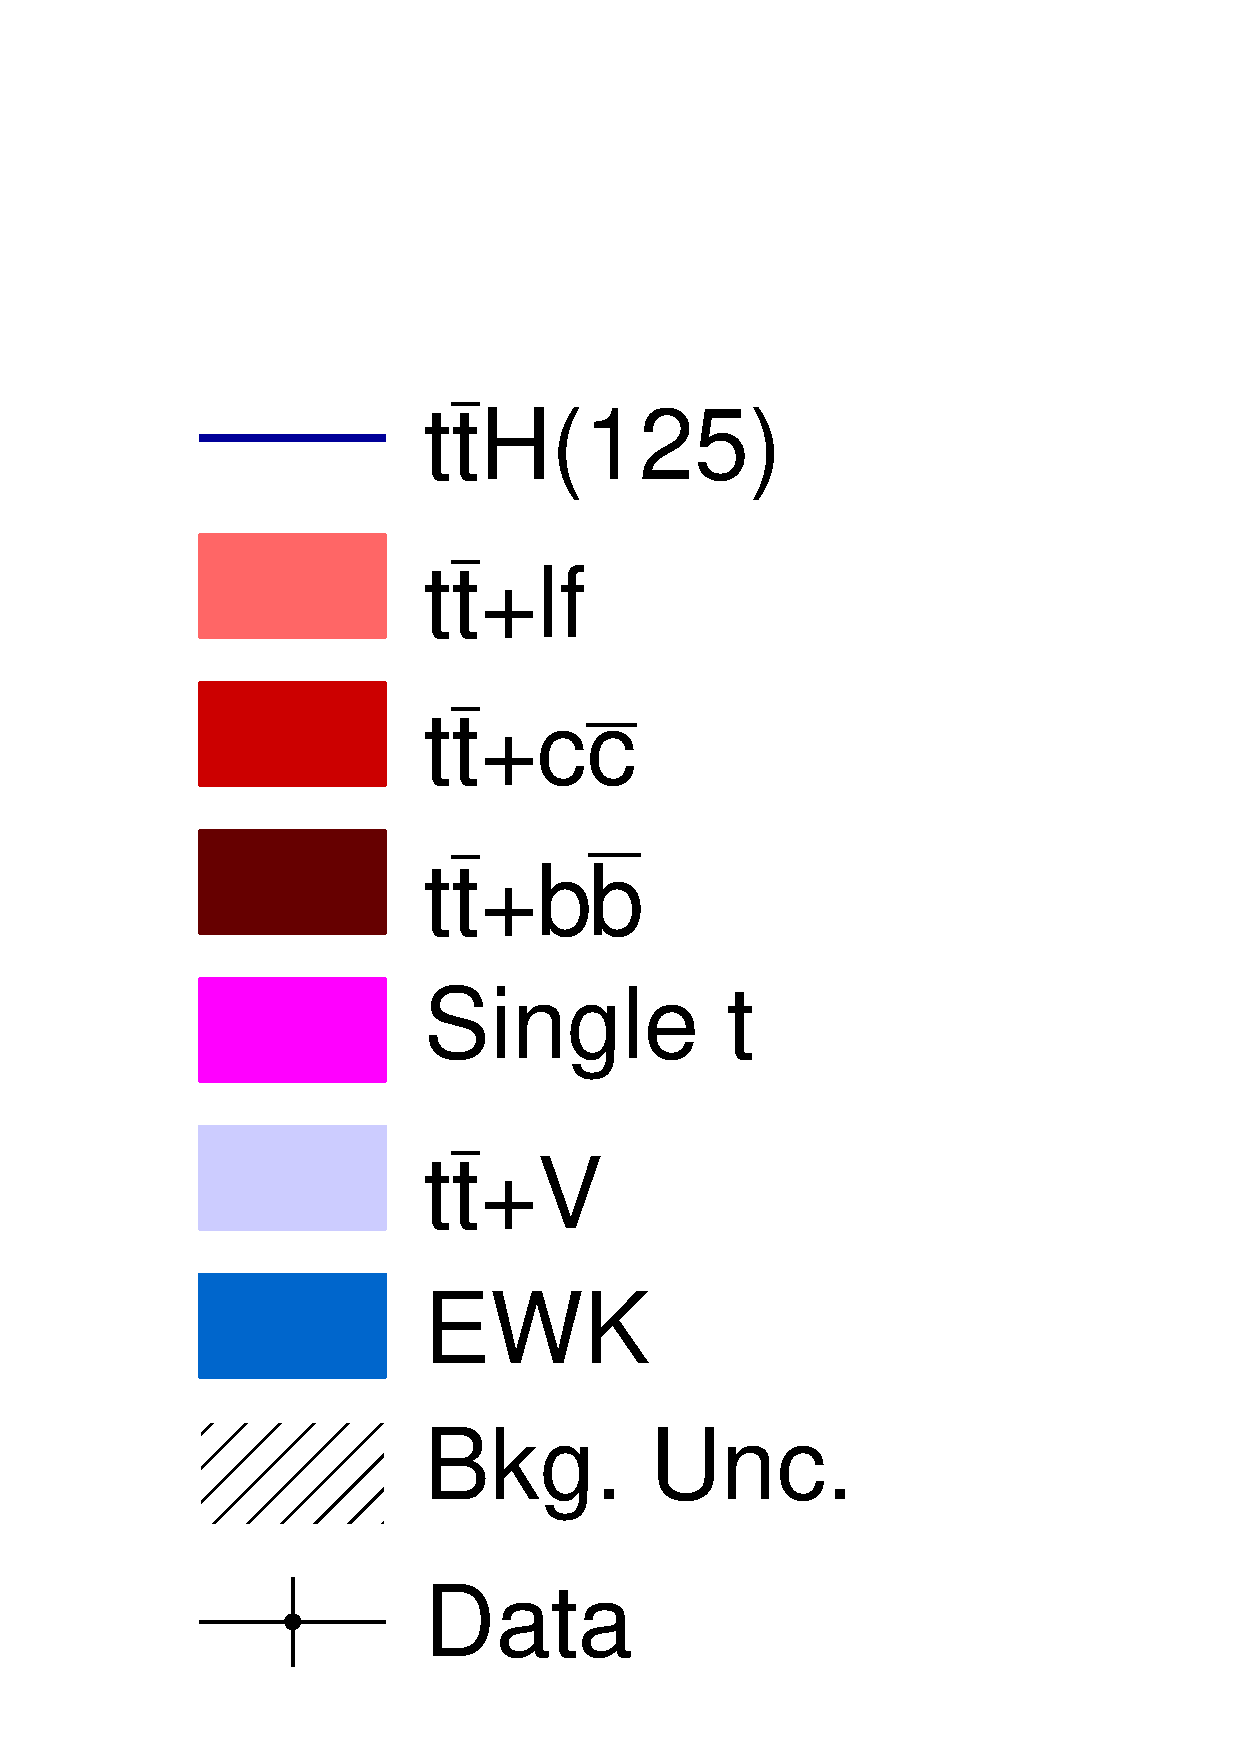
\includegraphics[width=0.25\textwidth]{Figures/Analysis_1_Diagrams/samples_legend_tall_noTTHscale.pdf}}
   \hspace{0.055\textwidth}
   \caption{Lepton + jets data/MC comparison for the $\ge$ 6 jets + 2 tag category.  The uncertainty band includes statistical and systematic uncertainties that affect both the rate and shape of the background distributions.}
   \label{fig:lj_input_6j_2t_part2}
 \end{center}
\end{figure}


%%%%%%%%%%%%%%%%%%%%%%%%%%%%%%%%%%%%%%%%%%%%%%%%%%%%%%%%%%%%%%%
%
%  NN Inputs 4j3t L+J (muon+electron) 8TeV
%
%%%%%%%%%%%%%%%%%%%%%%%%%%%%%%%%%%%%%%%%%%%%%%%%%%%%%%%%%%%%%%%

\clearpage

\begin{figure}[hbtp]
 \begin{center}
   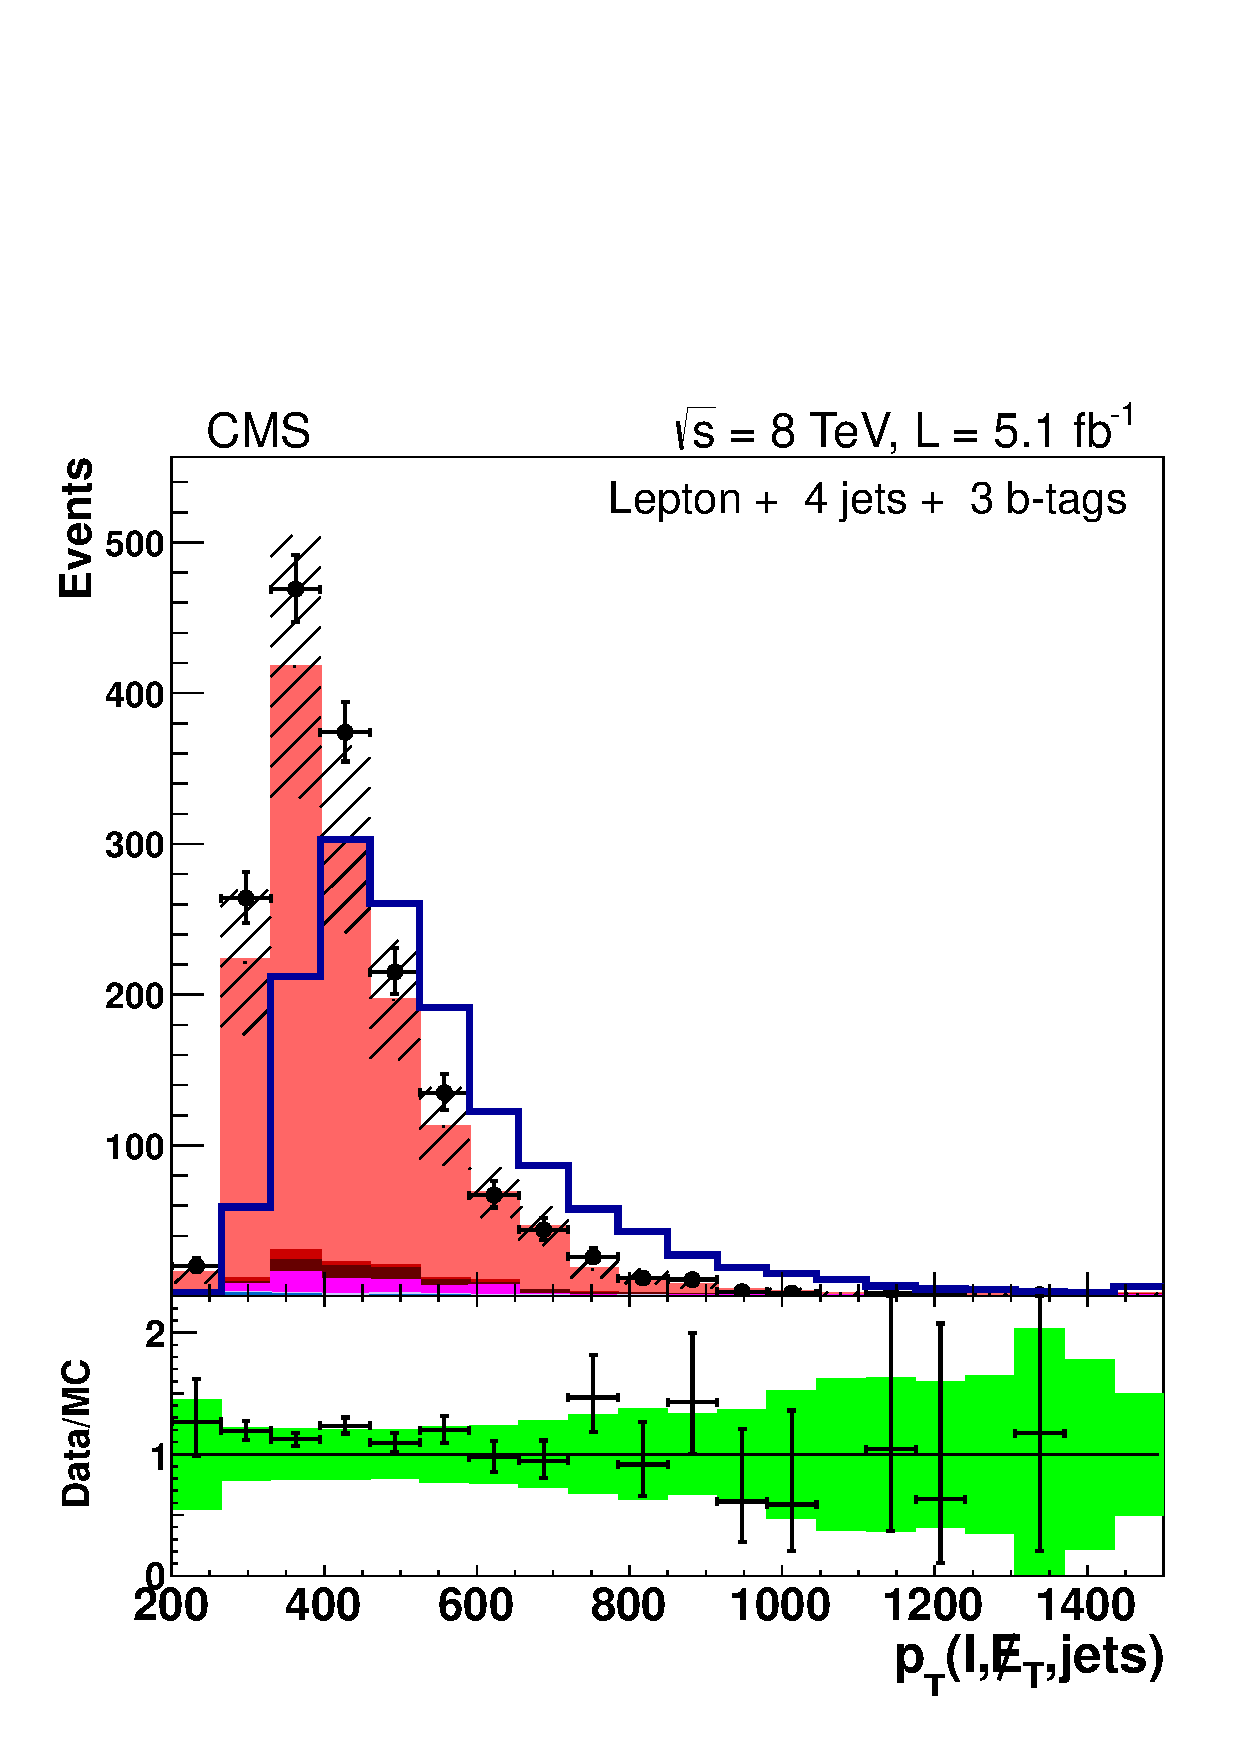
\includegraphics[width=0.31\textwidth]{Figures/Analysis_1_Diagrams/d2MCPlots_all_sum_pt_incl_met_cut4_j4_t3_Combined_HtWgt.pdf}
   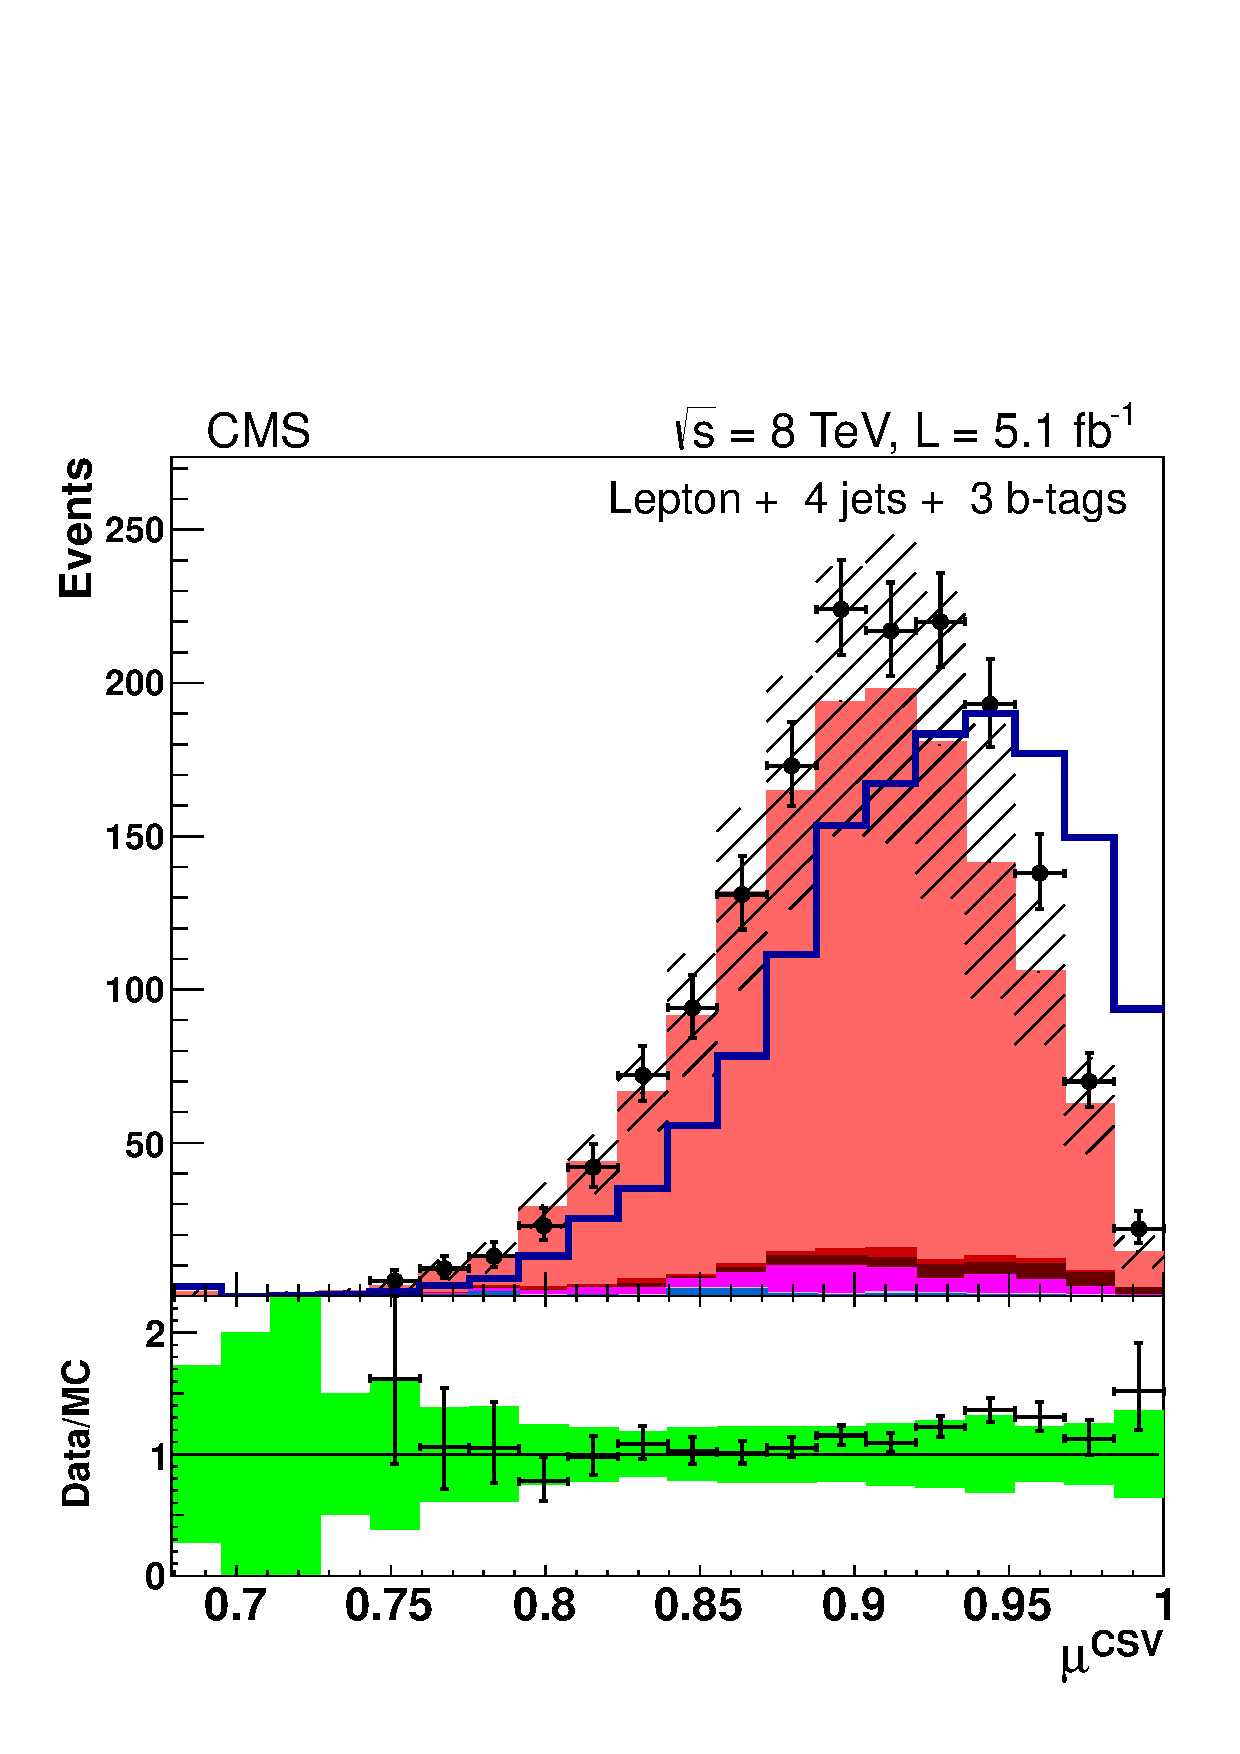
\includegraphics[width=0.31\textwidth]{Figures/Analysis_1_Diagrams/d2MCPlots_avg_btag_disc_btags_cut4_j4_t3_Combined_HtWgt.pdf}
   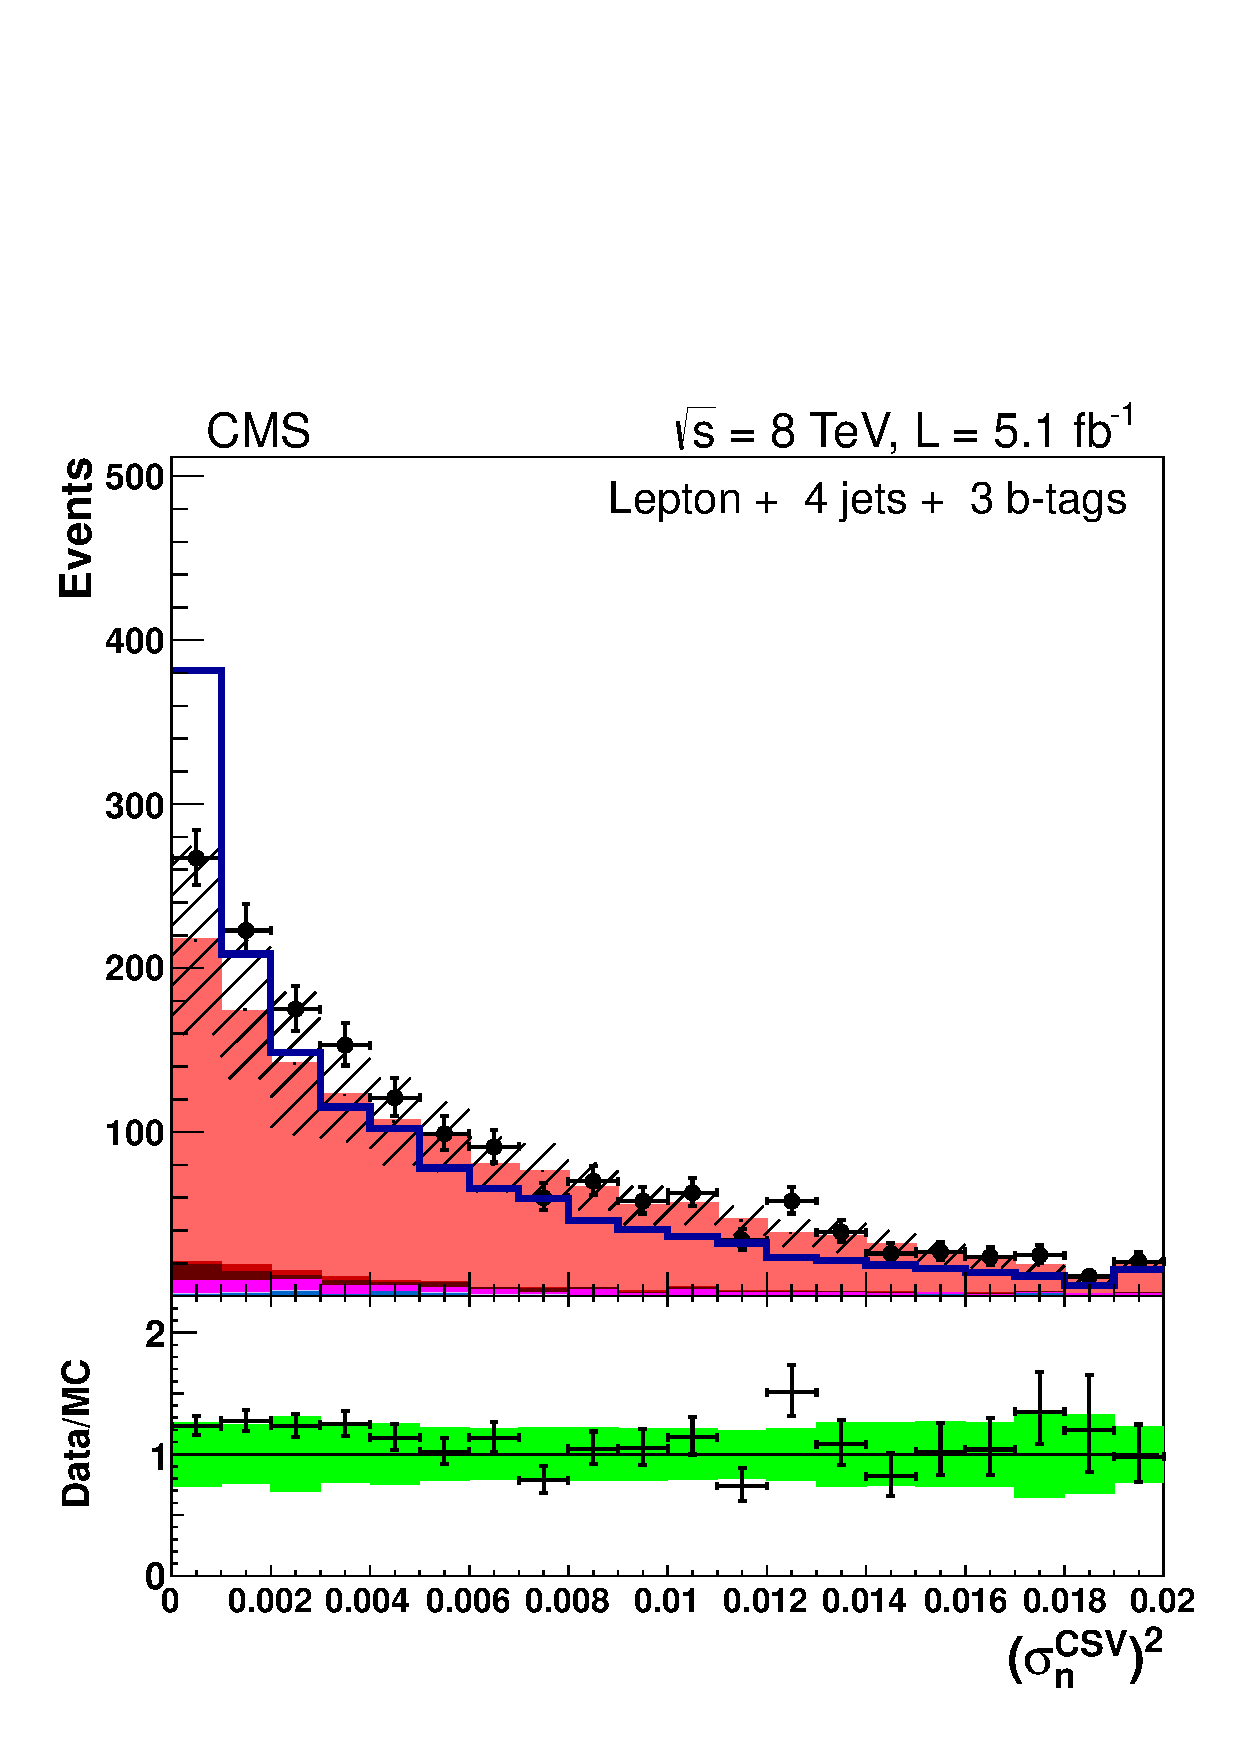
\includegraphics[width=0.31\textwidth]{Figures/Analysis_1_Diagrams/d2MCPlots_dev_from_avg_disc_btags_cut4_j4_t3_Combined_HtWgt.pdf}
   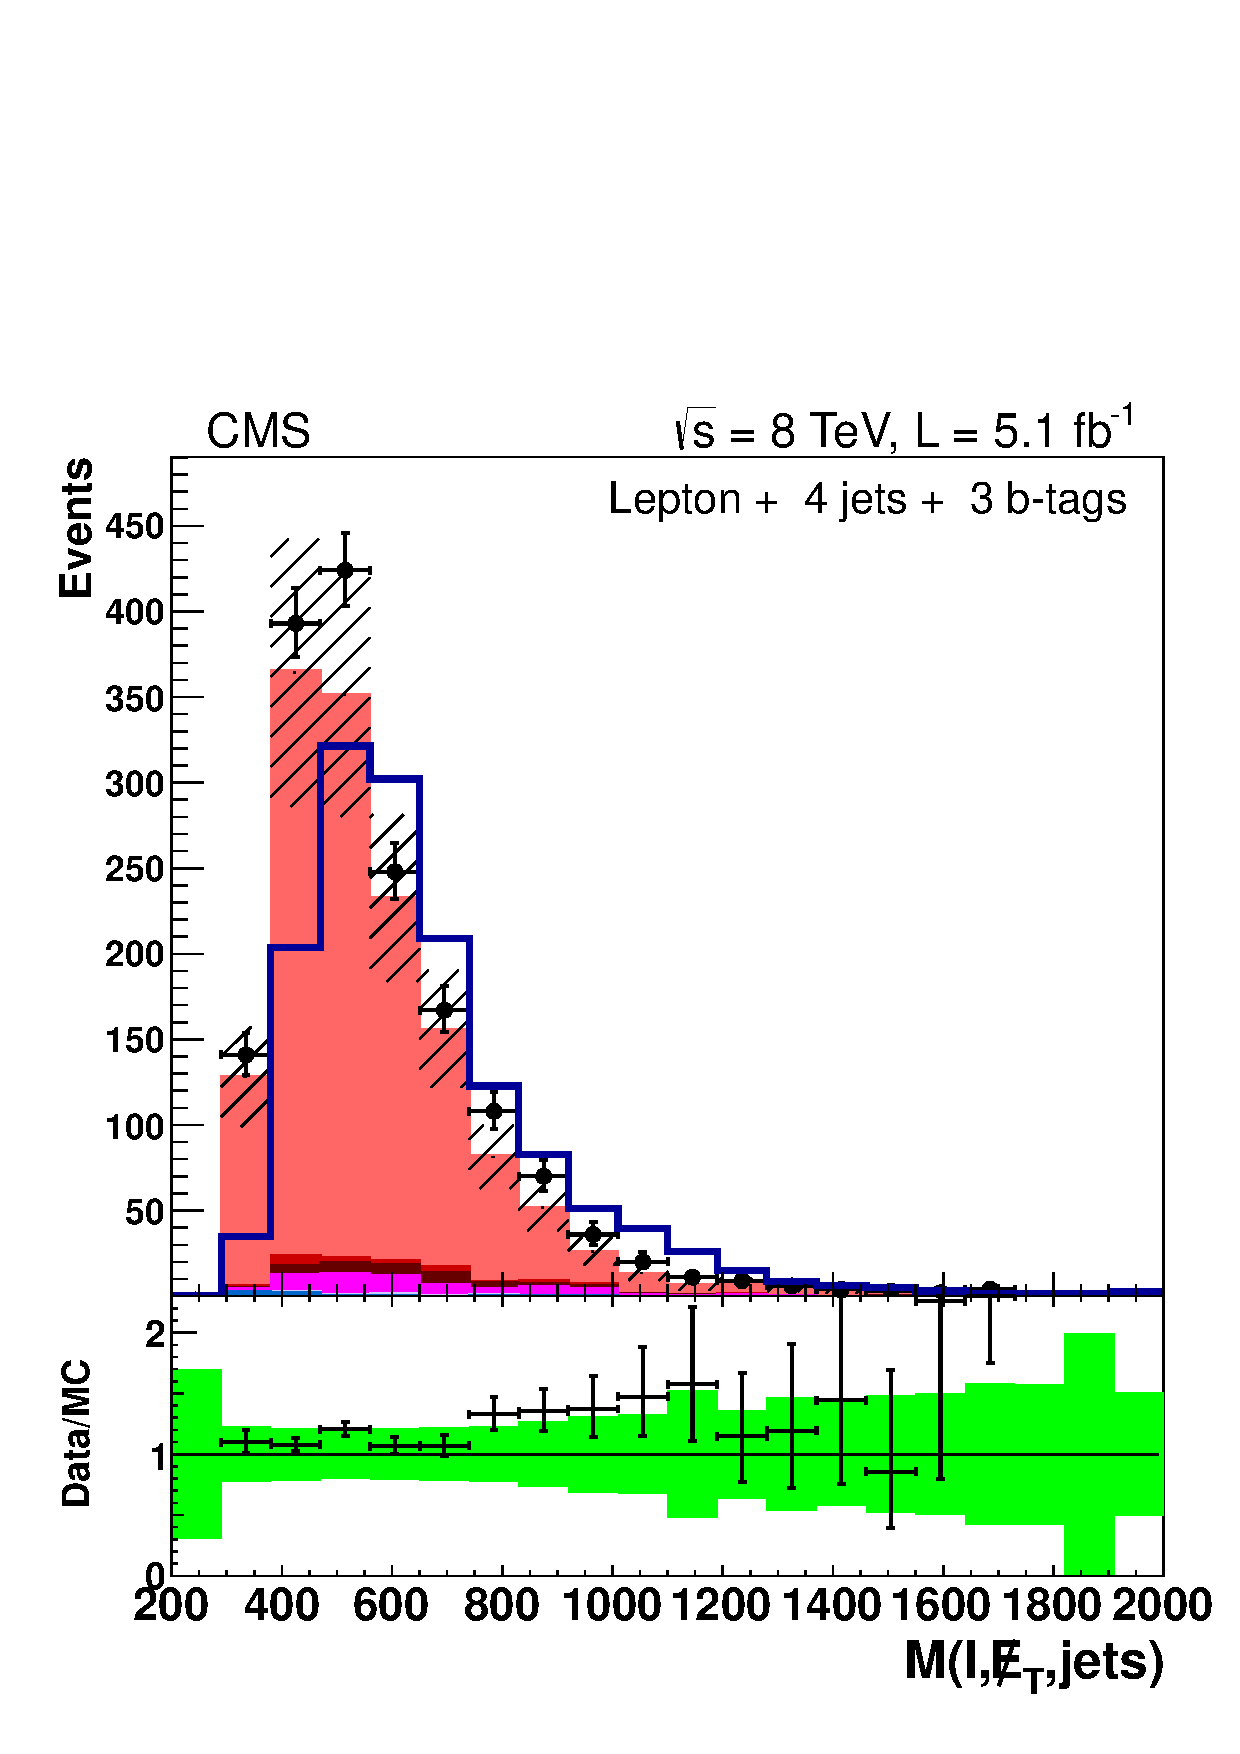
\includegraphics[width=0.31\textwidth]{Figures/Analysis_1_Diagrams/d2MCPlots_dijet_mass_of_everything_cut4_j4_t3_Combined_HtWgt.pdf}
   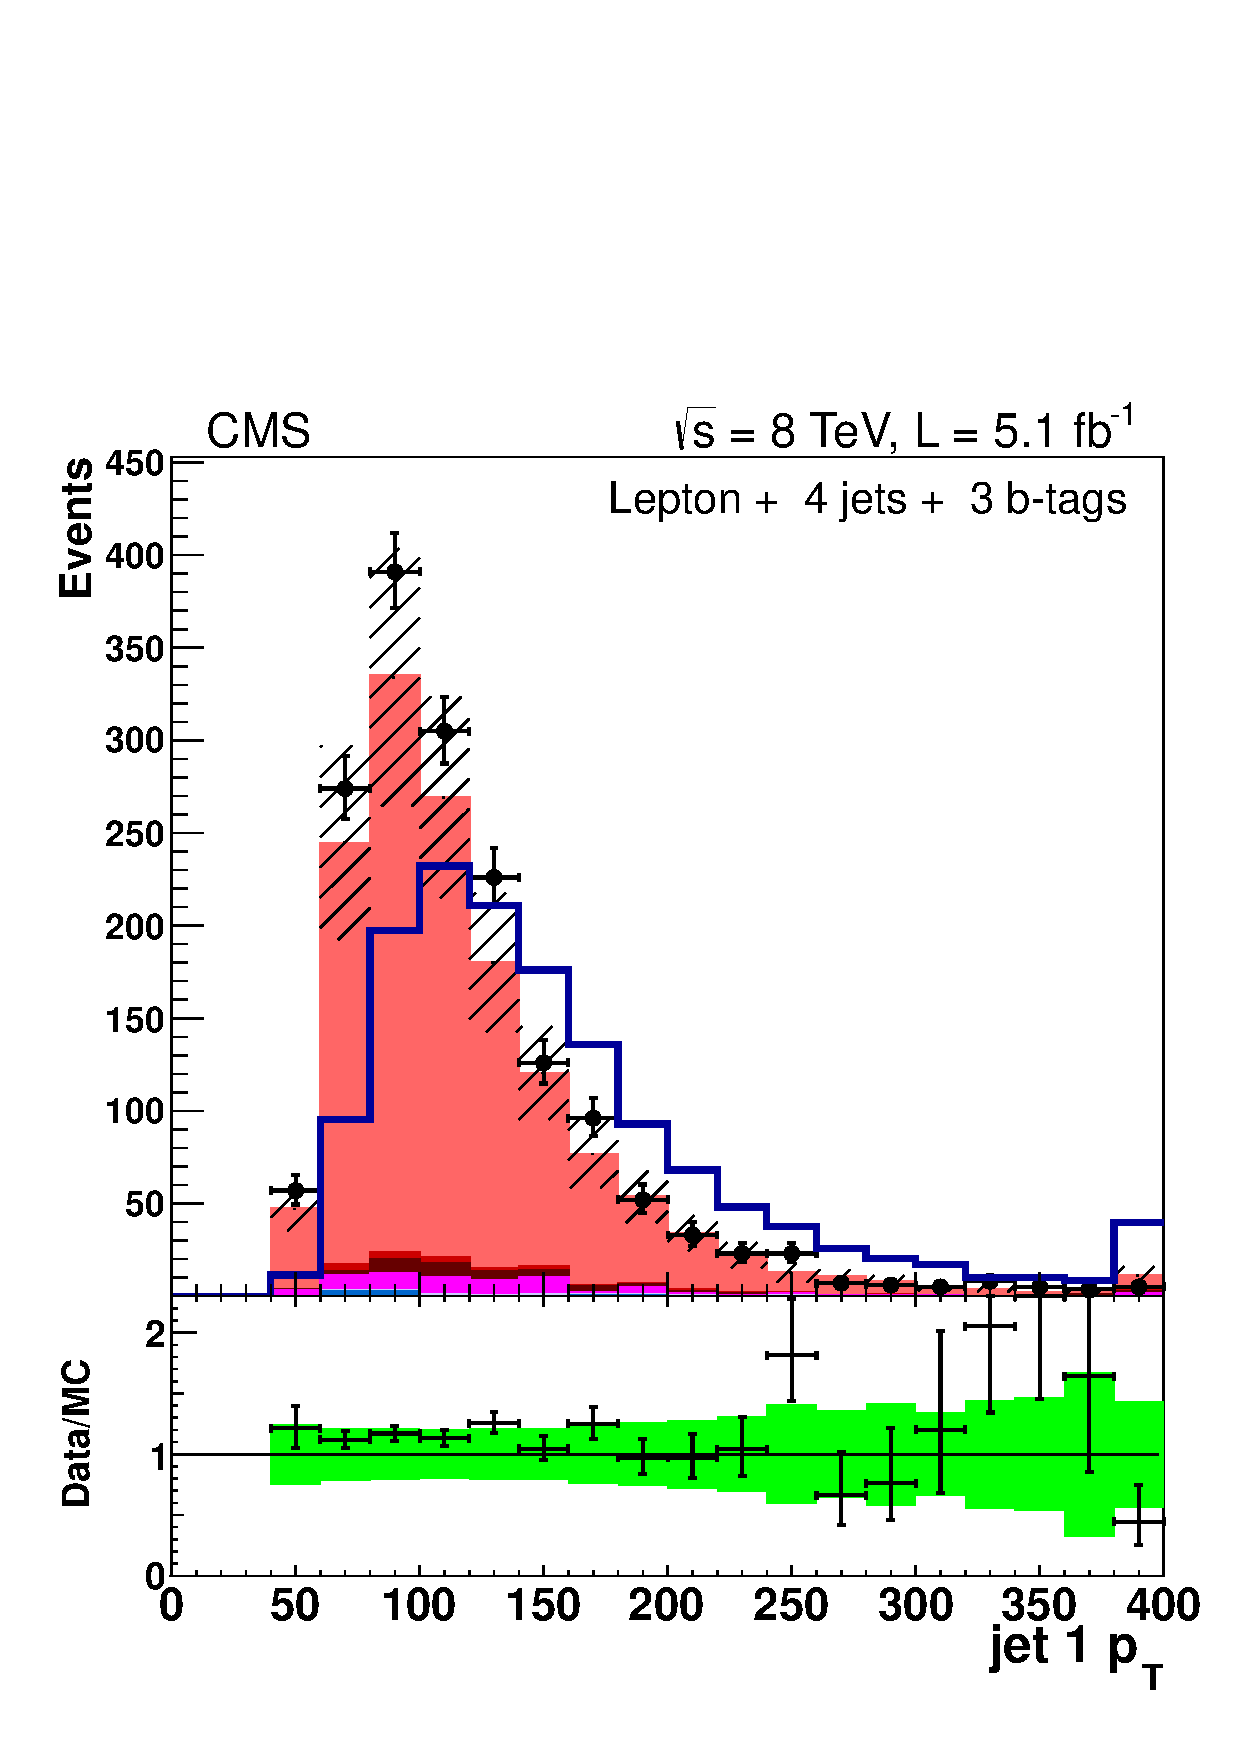
\includegraphics[width=0.31\textwidth]{Figures/Analysis_1_Diagrams/d2MCPlots_first_jet_pt_cut4_j4_t3_Combined_HtWgt.pdf}
   \raisebox{0.1\height}{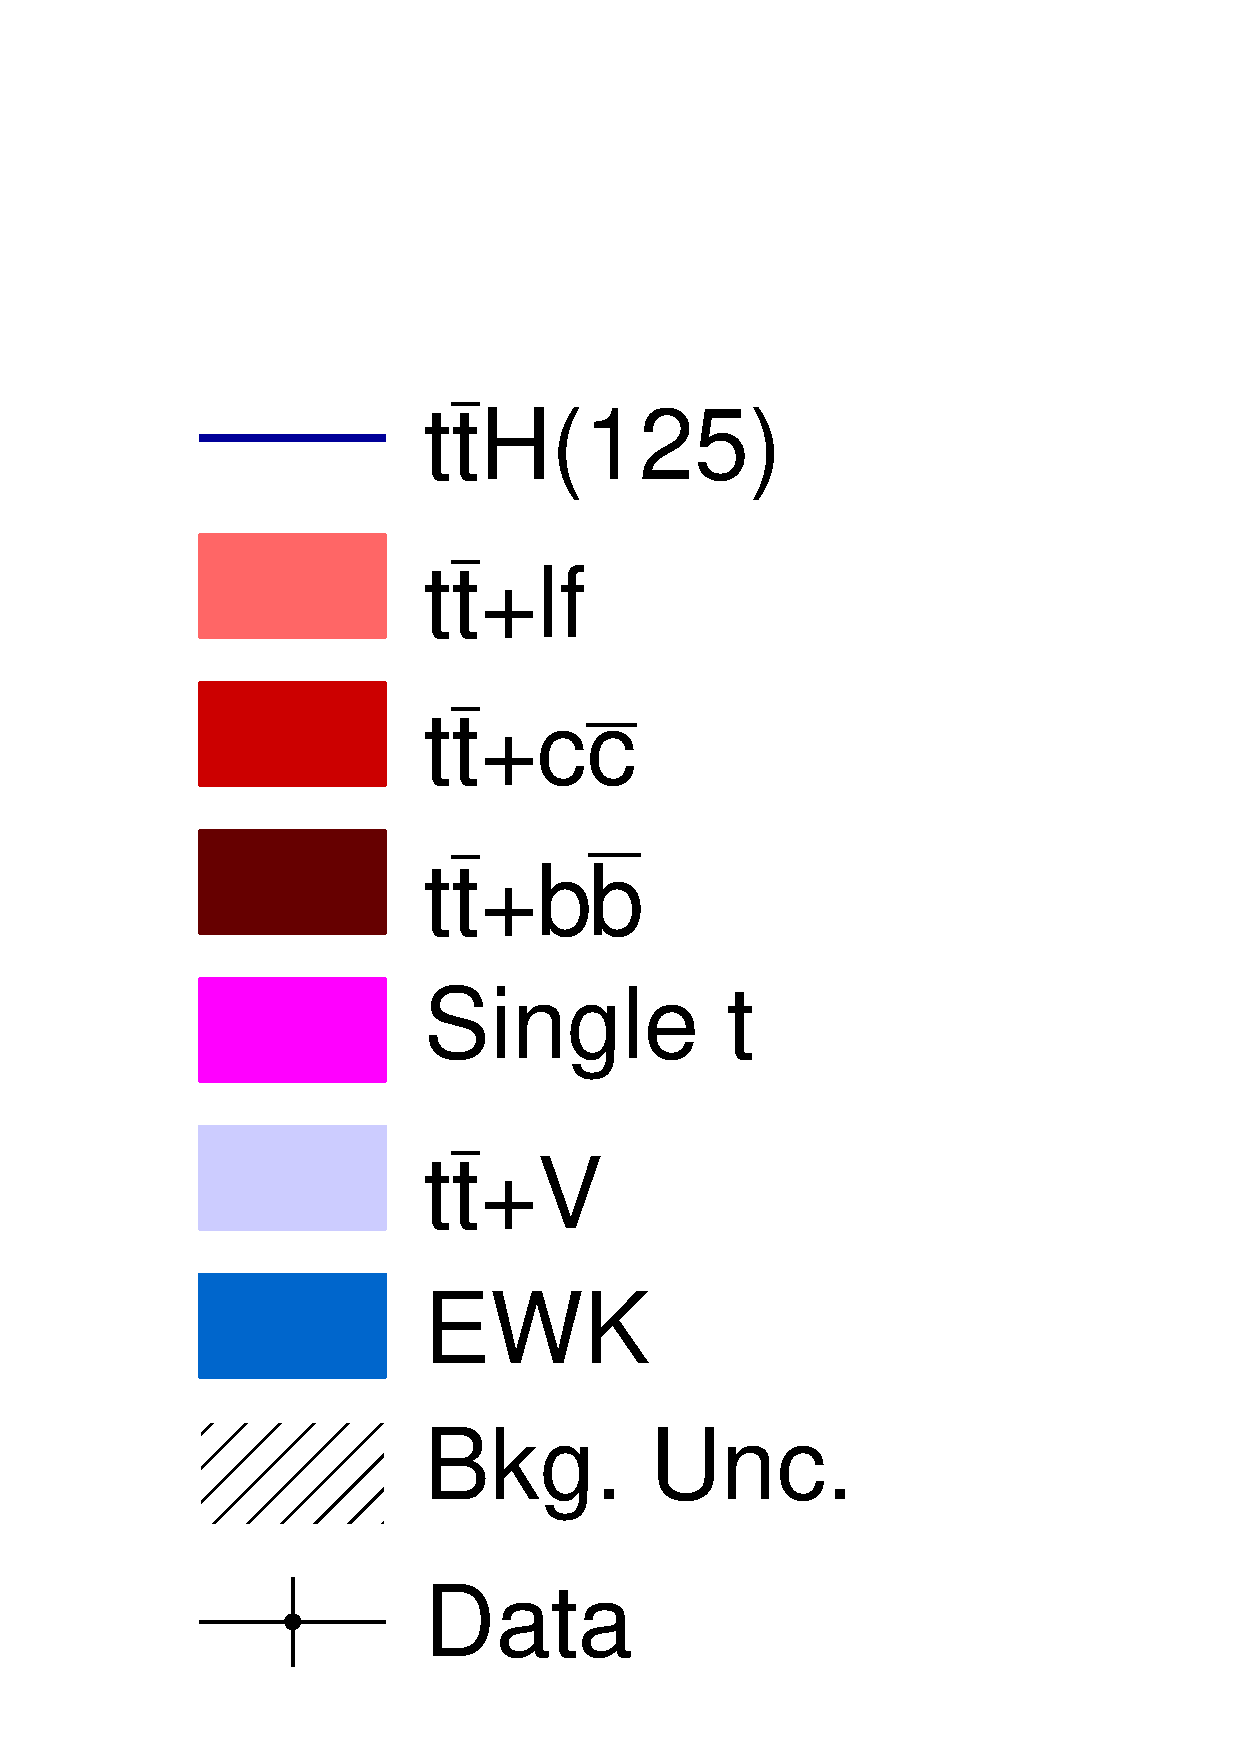
\includegraphics[width=0.25\textwidth]{Figures/Analysis_1_Diagrams/samples_legend_tall_noTTHscale.pdf}}
   \hspace{0.055\textwidth}
   \caption{Lepton + jets data/MC comparison for the 4 jets + 3 tag category.  The uncertainty band includes statistical and systematic uncertainties that affect both the rate and shape of the background distributions.}
   \label{fig:lj_input_4j_3t_part1}
 \end{center}
\end{figure}

\clearpage

\begin{figure}[hbtp]
 \begin{center}
   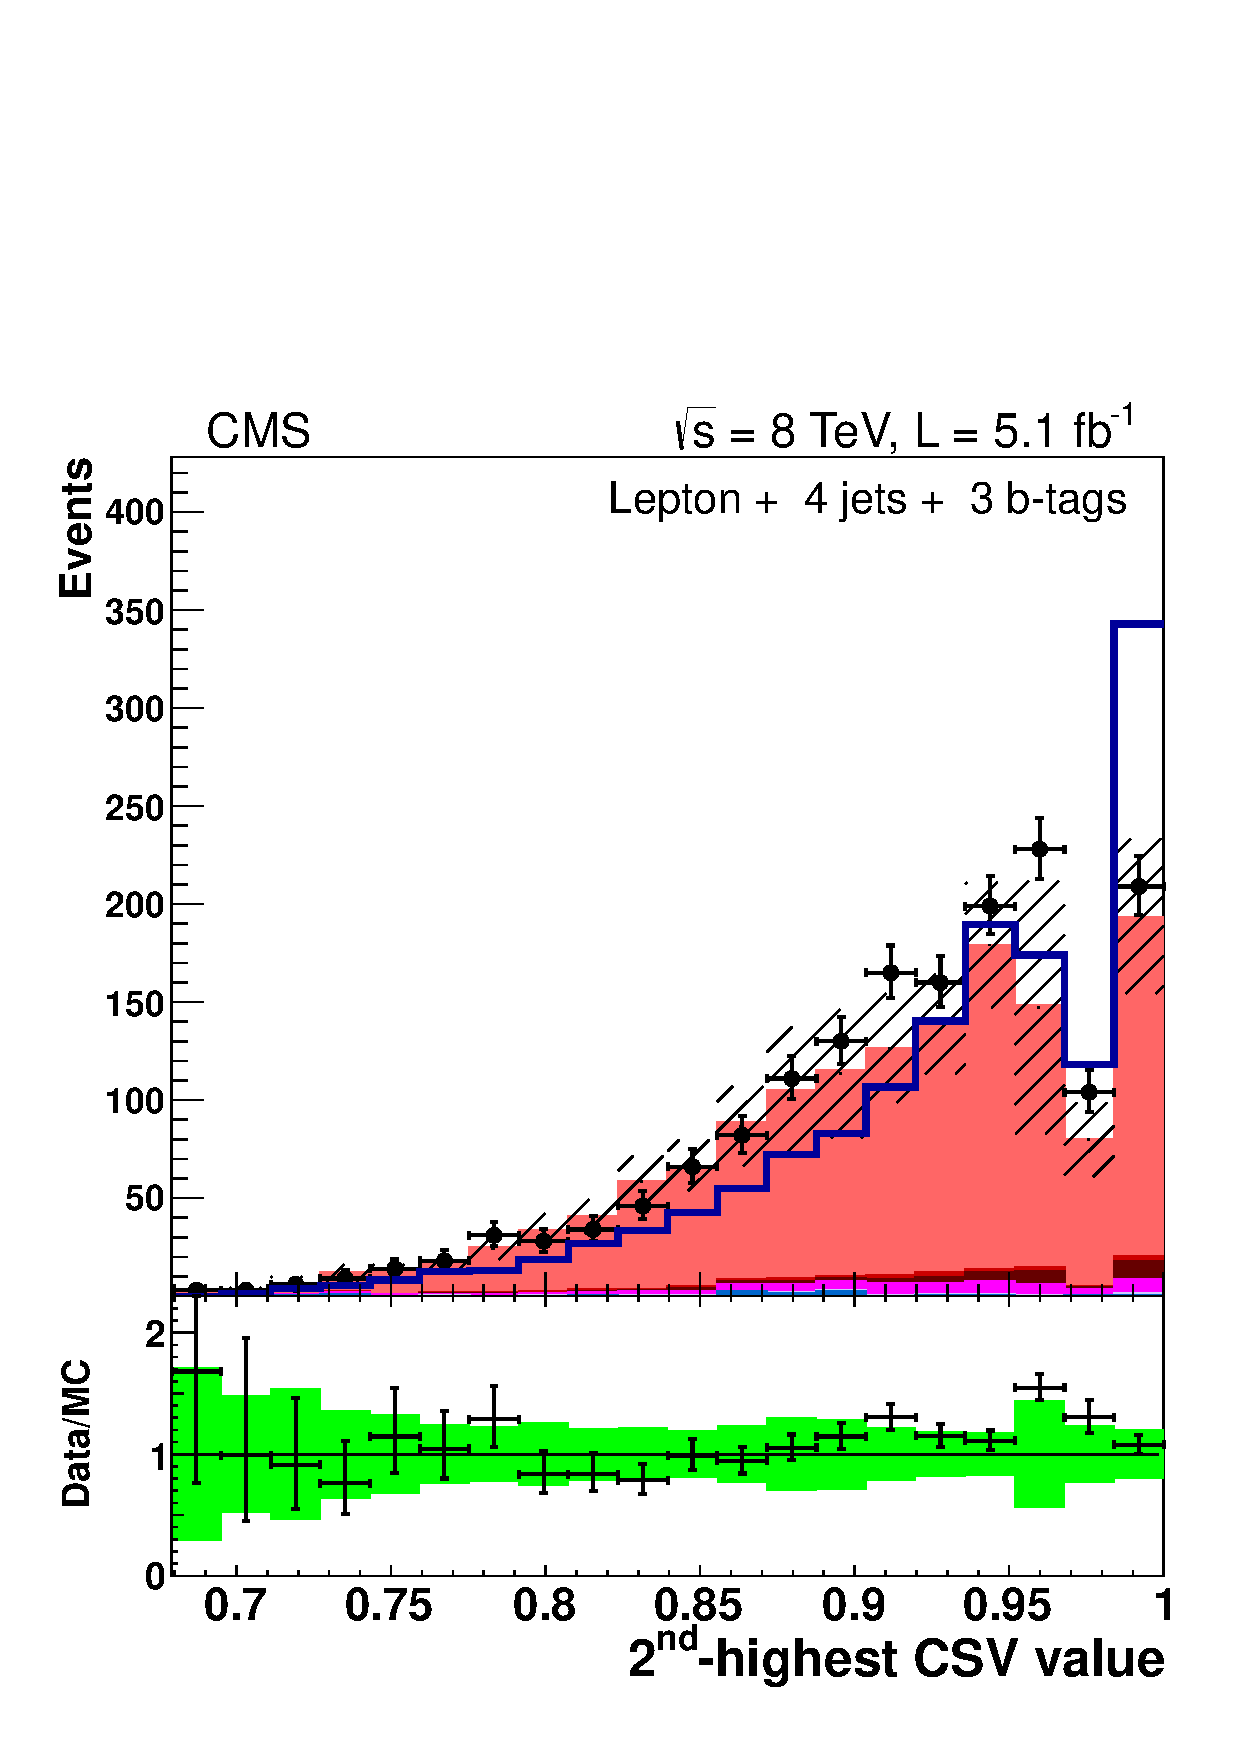
\includegraphics[width=0.31\textwidth]{Figures/Analysis_1_Diagrams/d2MCPlots_second_highest_btag_cut4_j4_t3_Combined_HtWgt.pdf}
   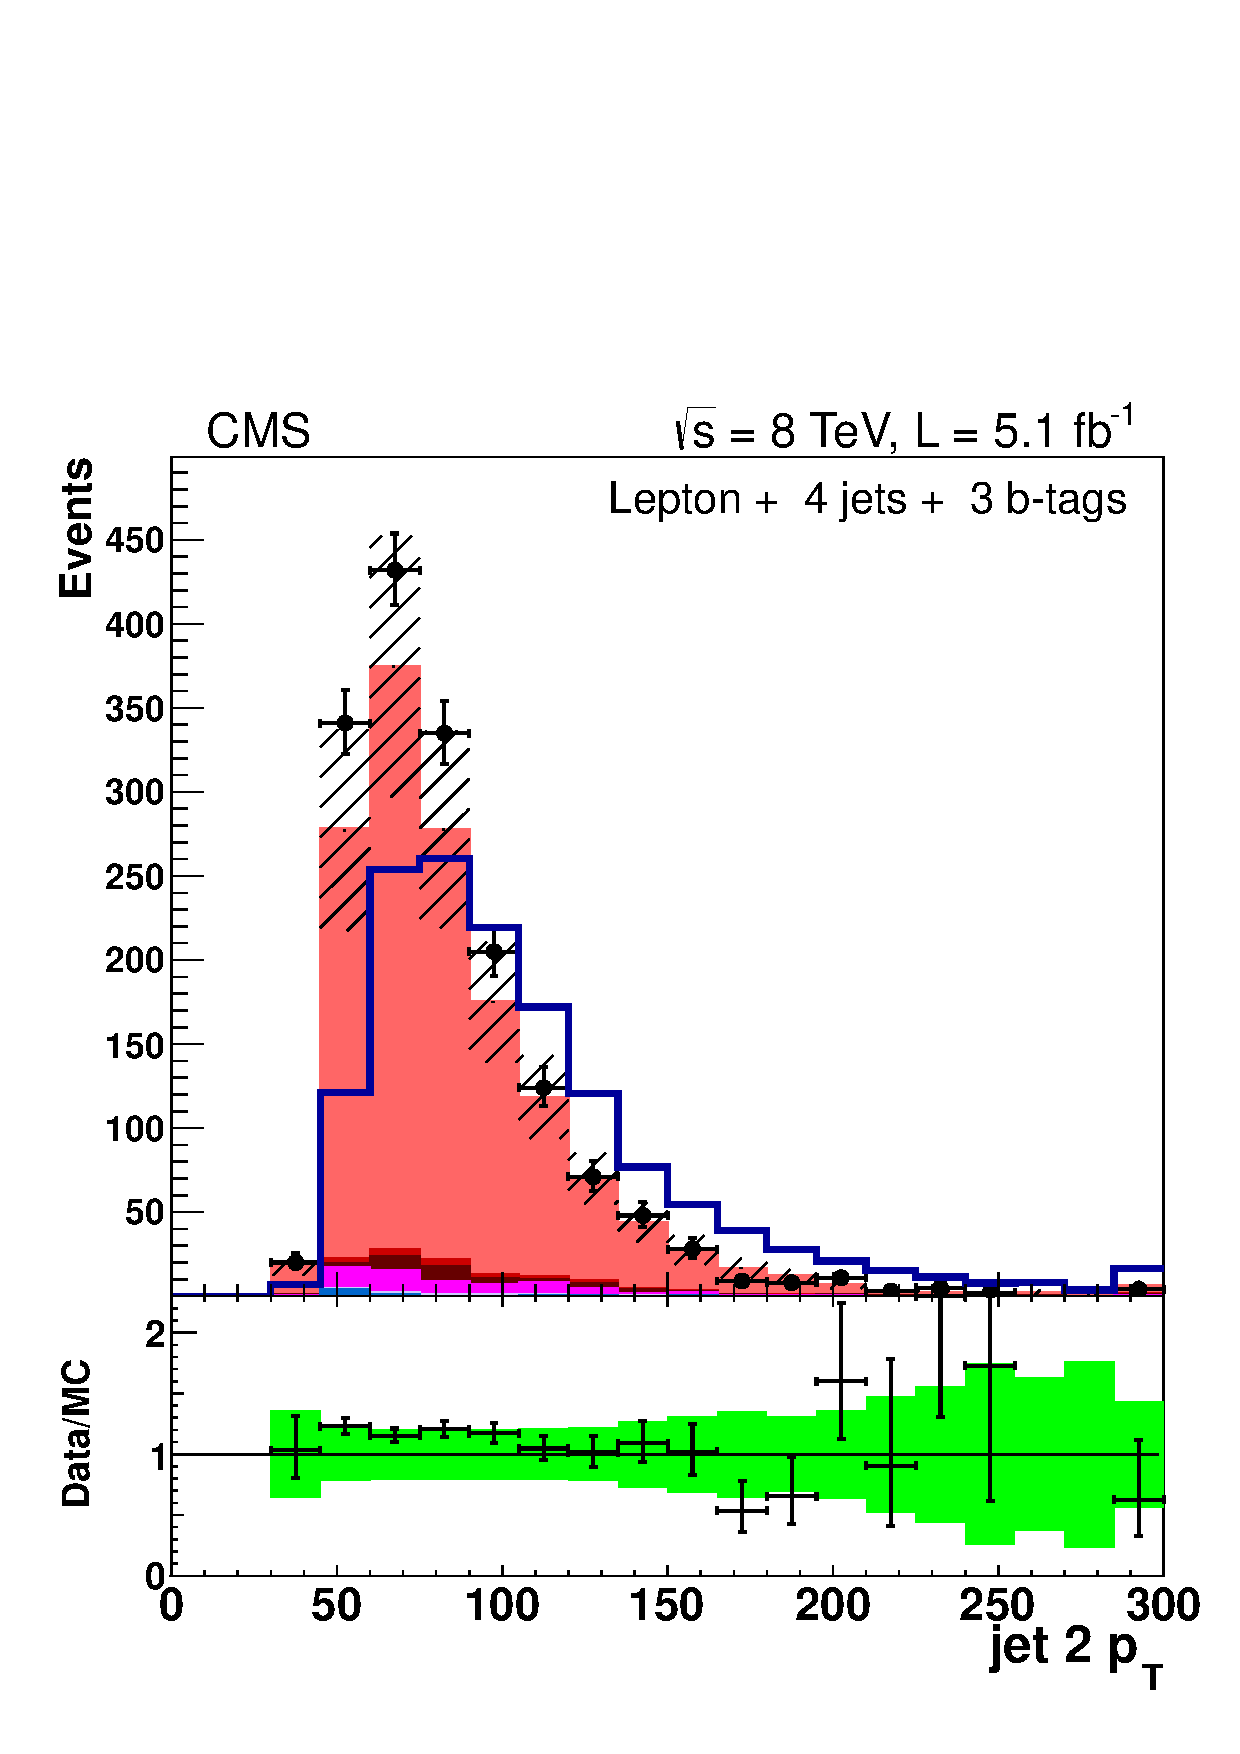
\includegraphics[width=0.31\textwidth]{Figures/Analysis_1_Diagrams/d2MCPlots_second_jet_pt_cut4_j4_t3_Combined_HtWgt.pdf}
   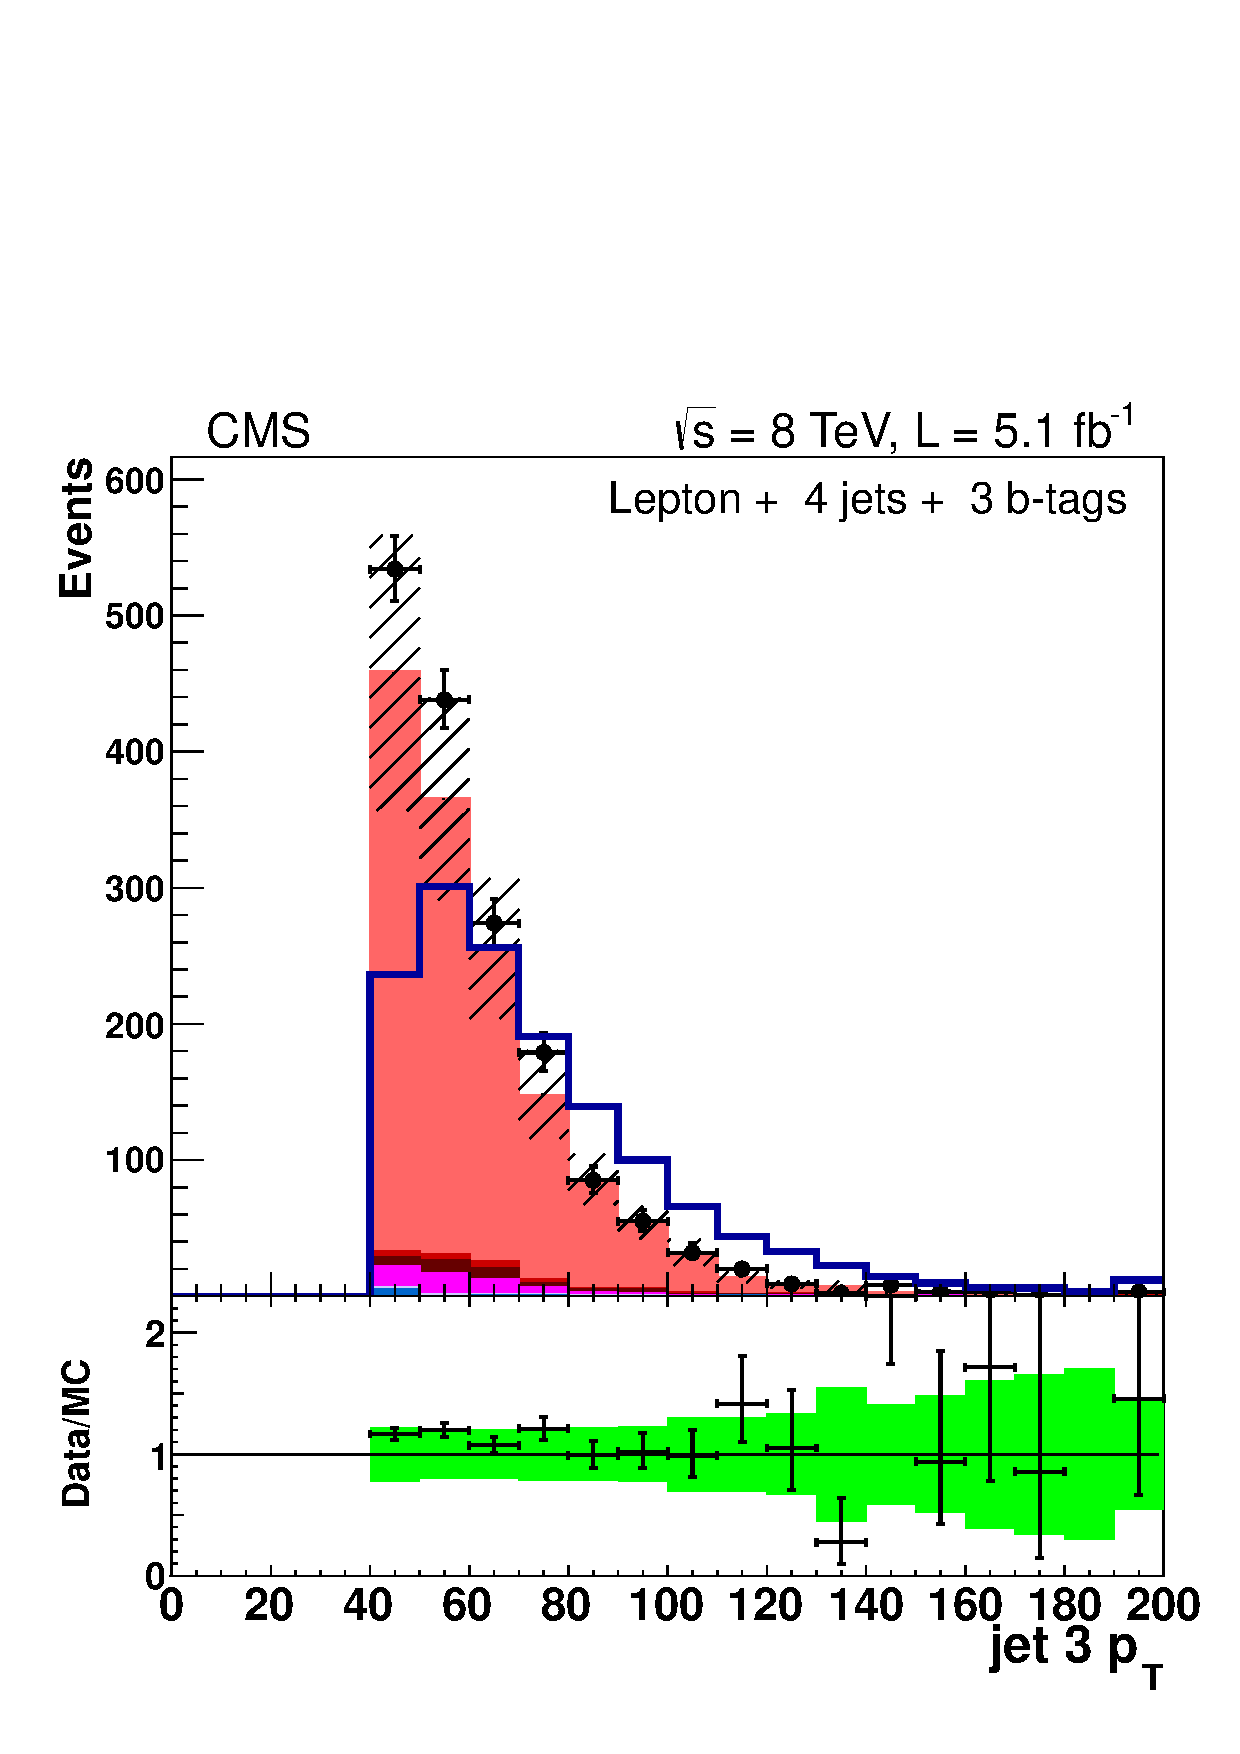
\includegraphics[width=0.31\textwidth]{Figures/Analysis_1_Diagrams/d2MCPlots_third_jet_pt_cut4_j4_t3_Combined_HtWgt.pdf}
   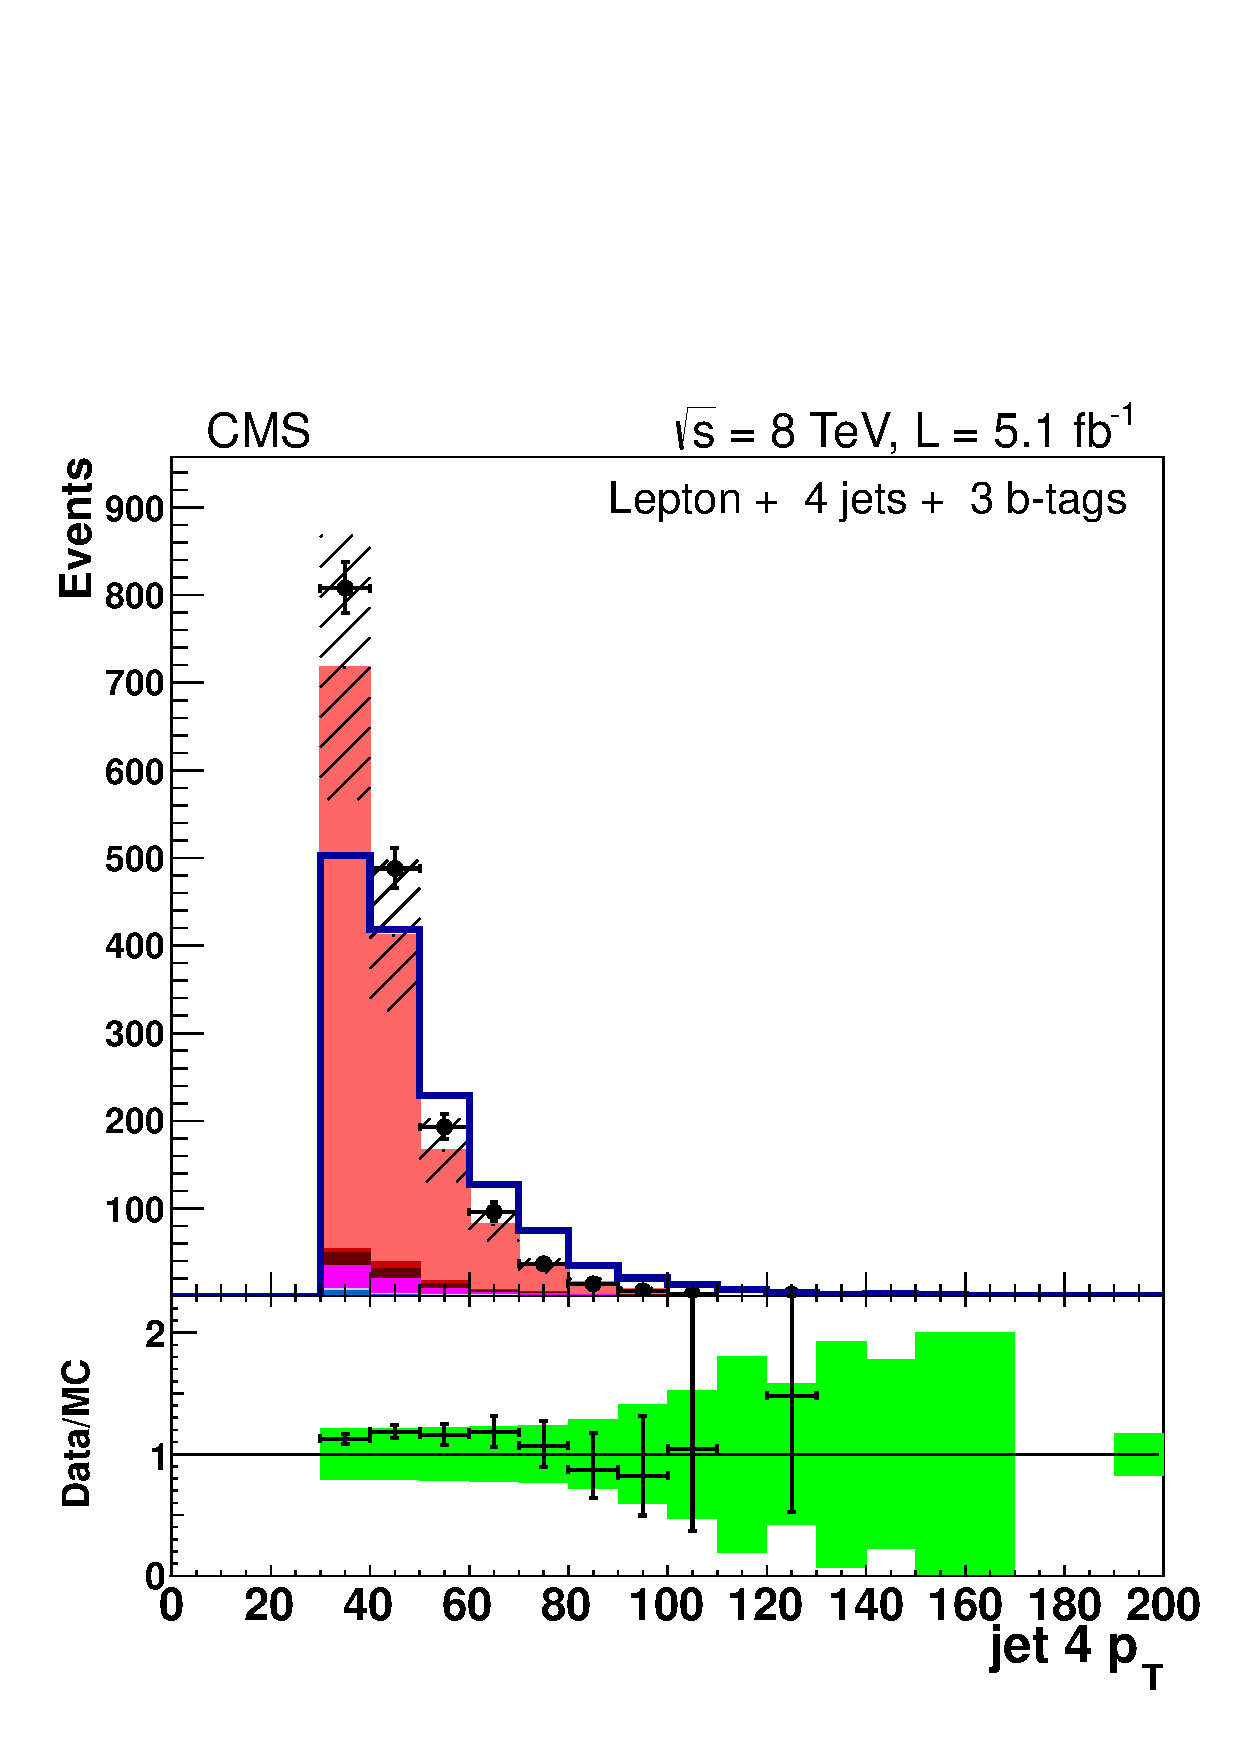
\includegraphics[width=0.31\textwidth]{Figures/Analysis_1_Diagrams/d2MCPlots_fourth_jet_pt_cut4_j4_t3_Combined_HtWgt.pdf}
   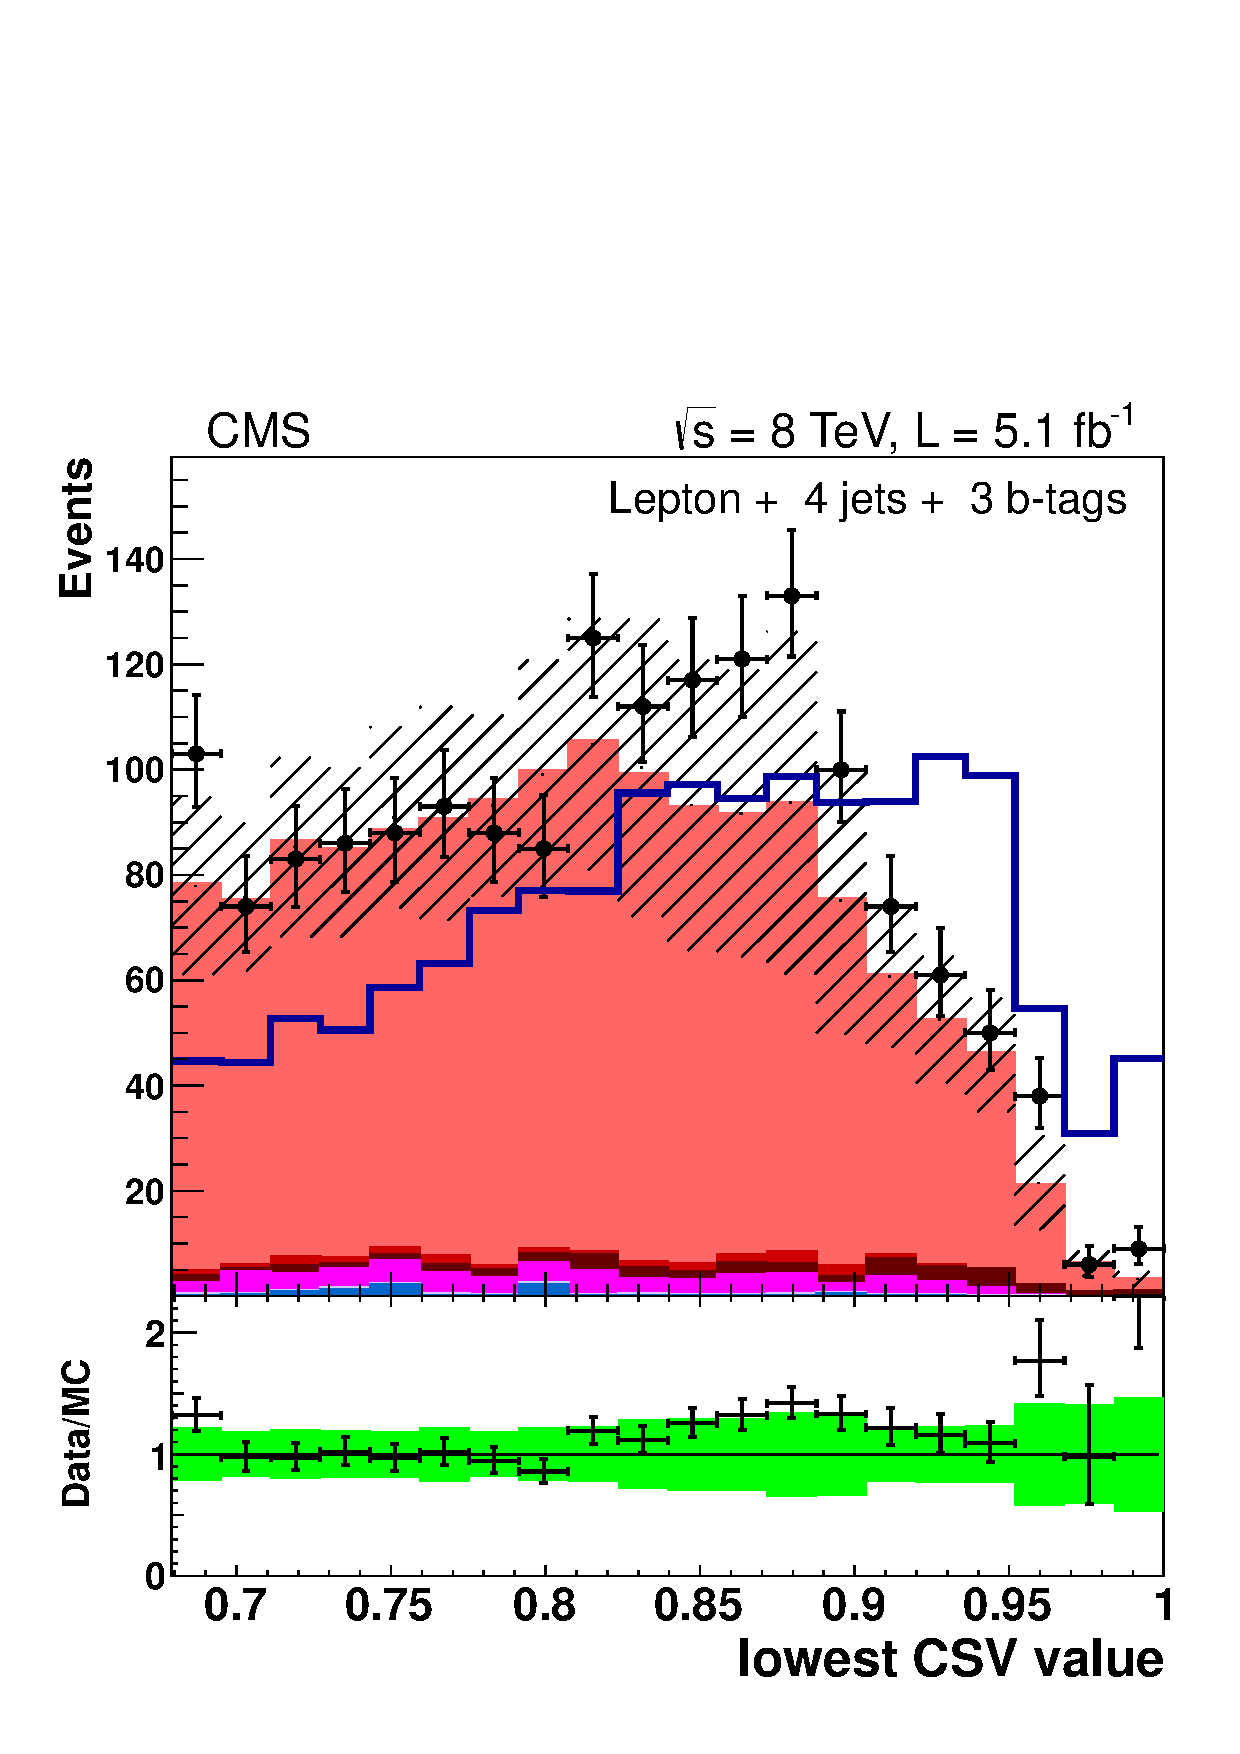
\includegraphics[width=0.31\textwidth]{Figures/Analysis_1_Diagrams/d2MCPlots_lowest_btag_cut4_j4_t3_Combined_HtWgt.pdf}
   \raisebox{0.1\height}{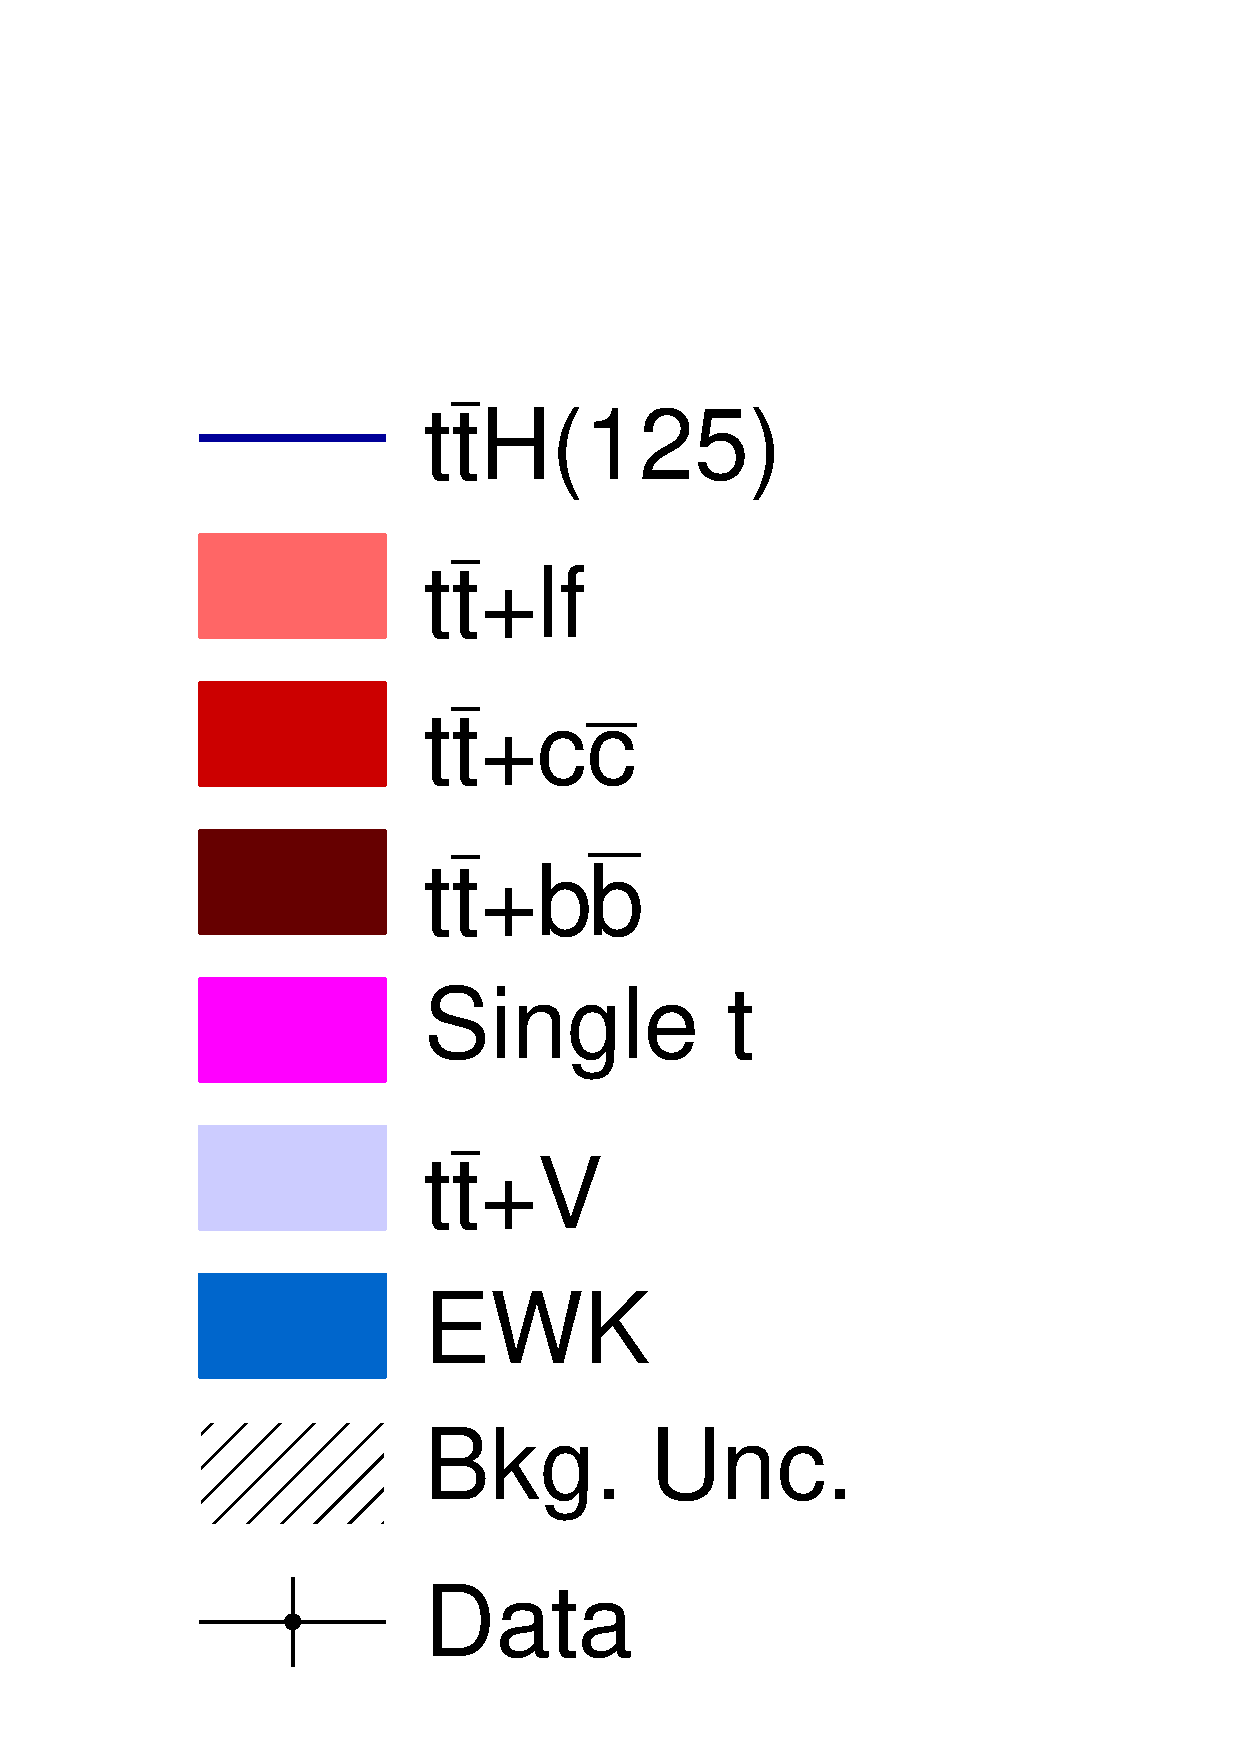
\includegraphics[width=0.25\textwidth]{Figures/Analysis_1_Diagrams/samples_legend_tall_noTTHscale.pdf}}
   \hspace{0.055\textwidth}
   \caption{Lepton + jets data/MC comparison for the 4 jets + 3 tag category.  The uncertainty band includes statistical and systematic uncertainties that affect both the rate and shape of the background distributions.}
   \label{fig:lj_input_4j_3t_part2}
 \end{center}
\end{figure}

%%%%%%%%%%%%%%%%%%%%%%%%%%%%%%%%%%%%%%%%%%%%%%%%%%%%%%%%%%%%%%%
%
%  NN Inputs 5j3t L+J (muon+electron) 8TeV
%
%%%%%%%%%%%%%%%%%%%%%%%%%%%%%%%%%%%%%%%%%%%%%%%%%%%%%%%%%%%%%%%

\clearpage

\begin{figure}[hbtp]
 \begin{center}
   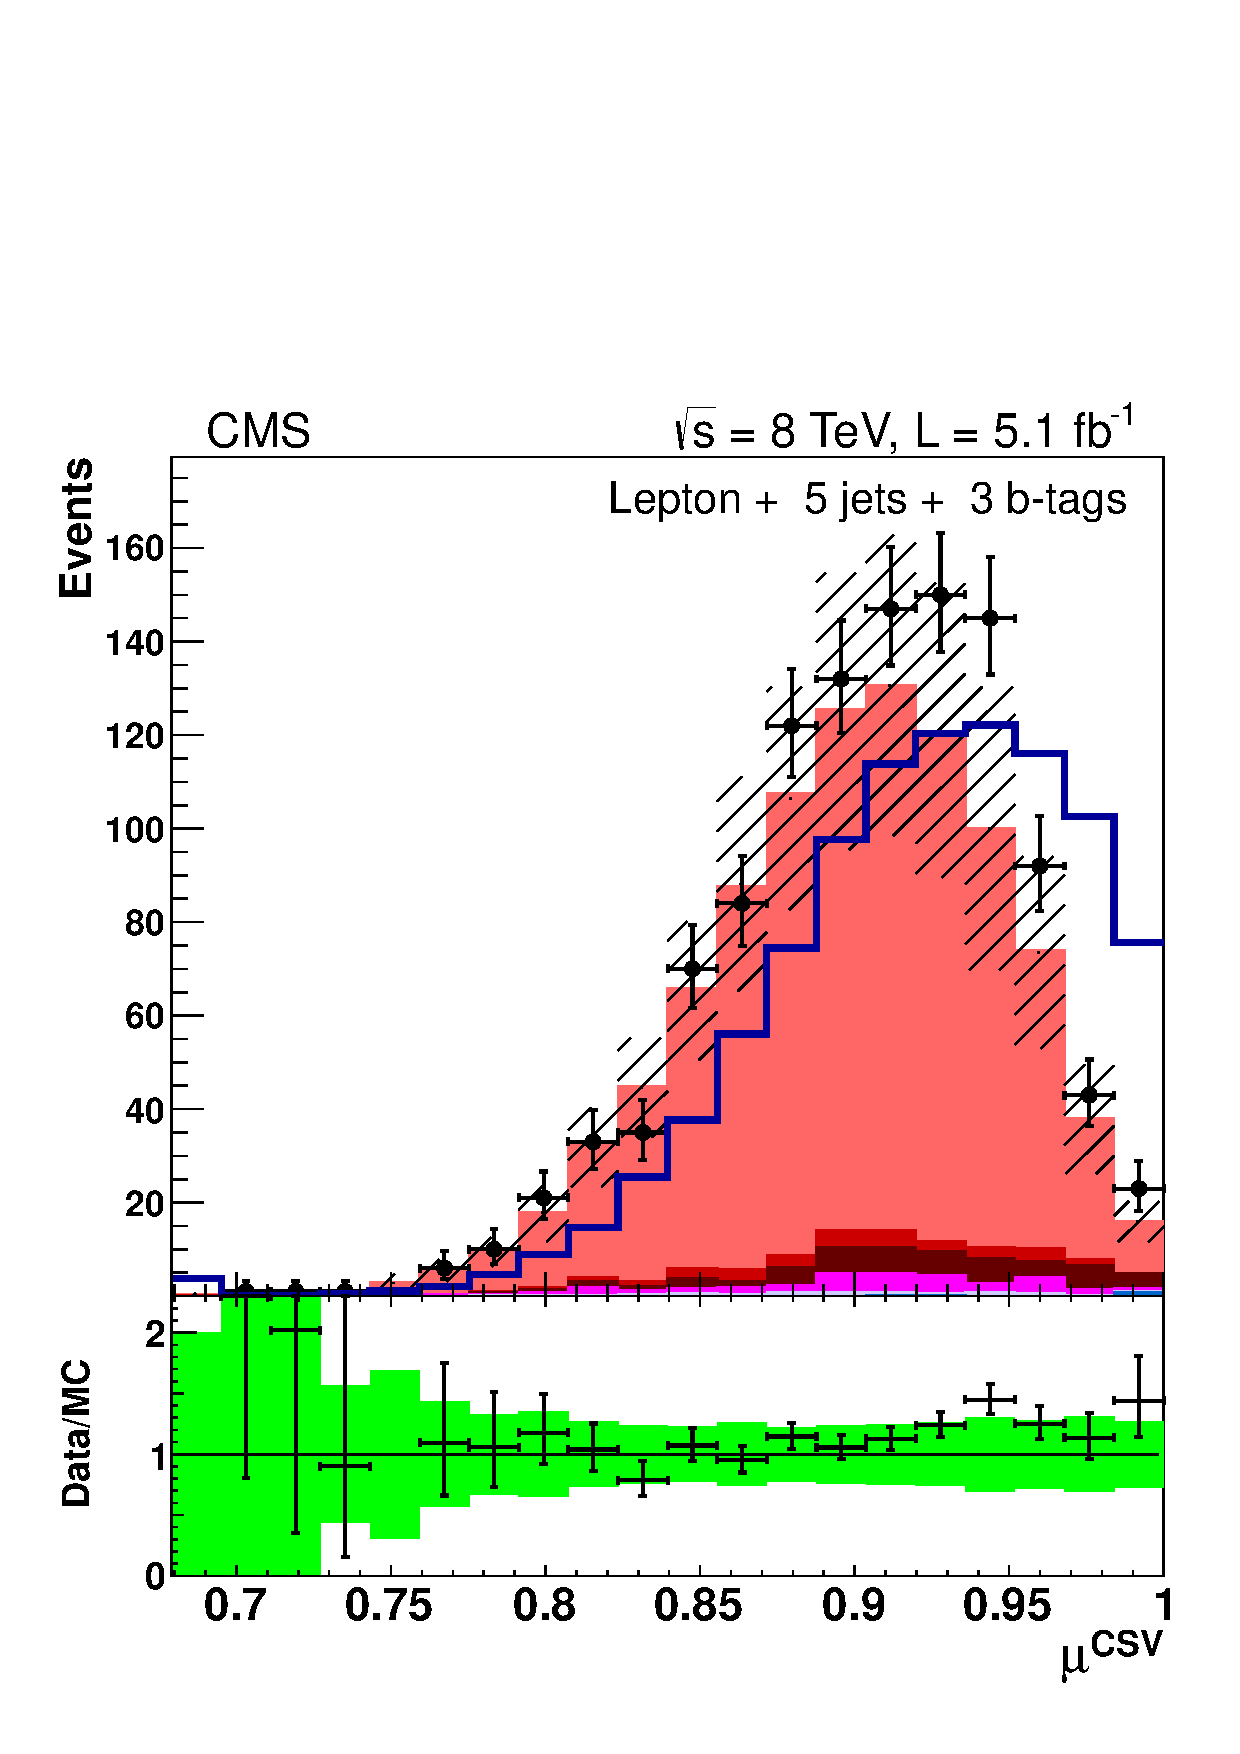
\includegraphics[width=0.31\textwidth]{Figures/Analysis_1_Diagrams/d2MCPlots_avg_btag_disc_btags_cut5_j5_t3_Combined_HtWgt.pdf}
   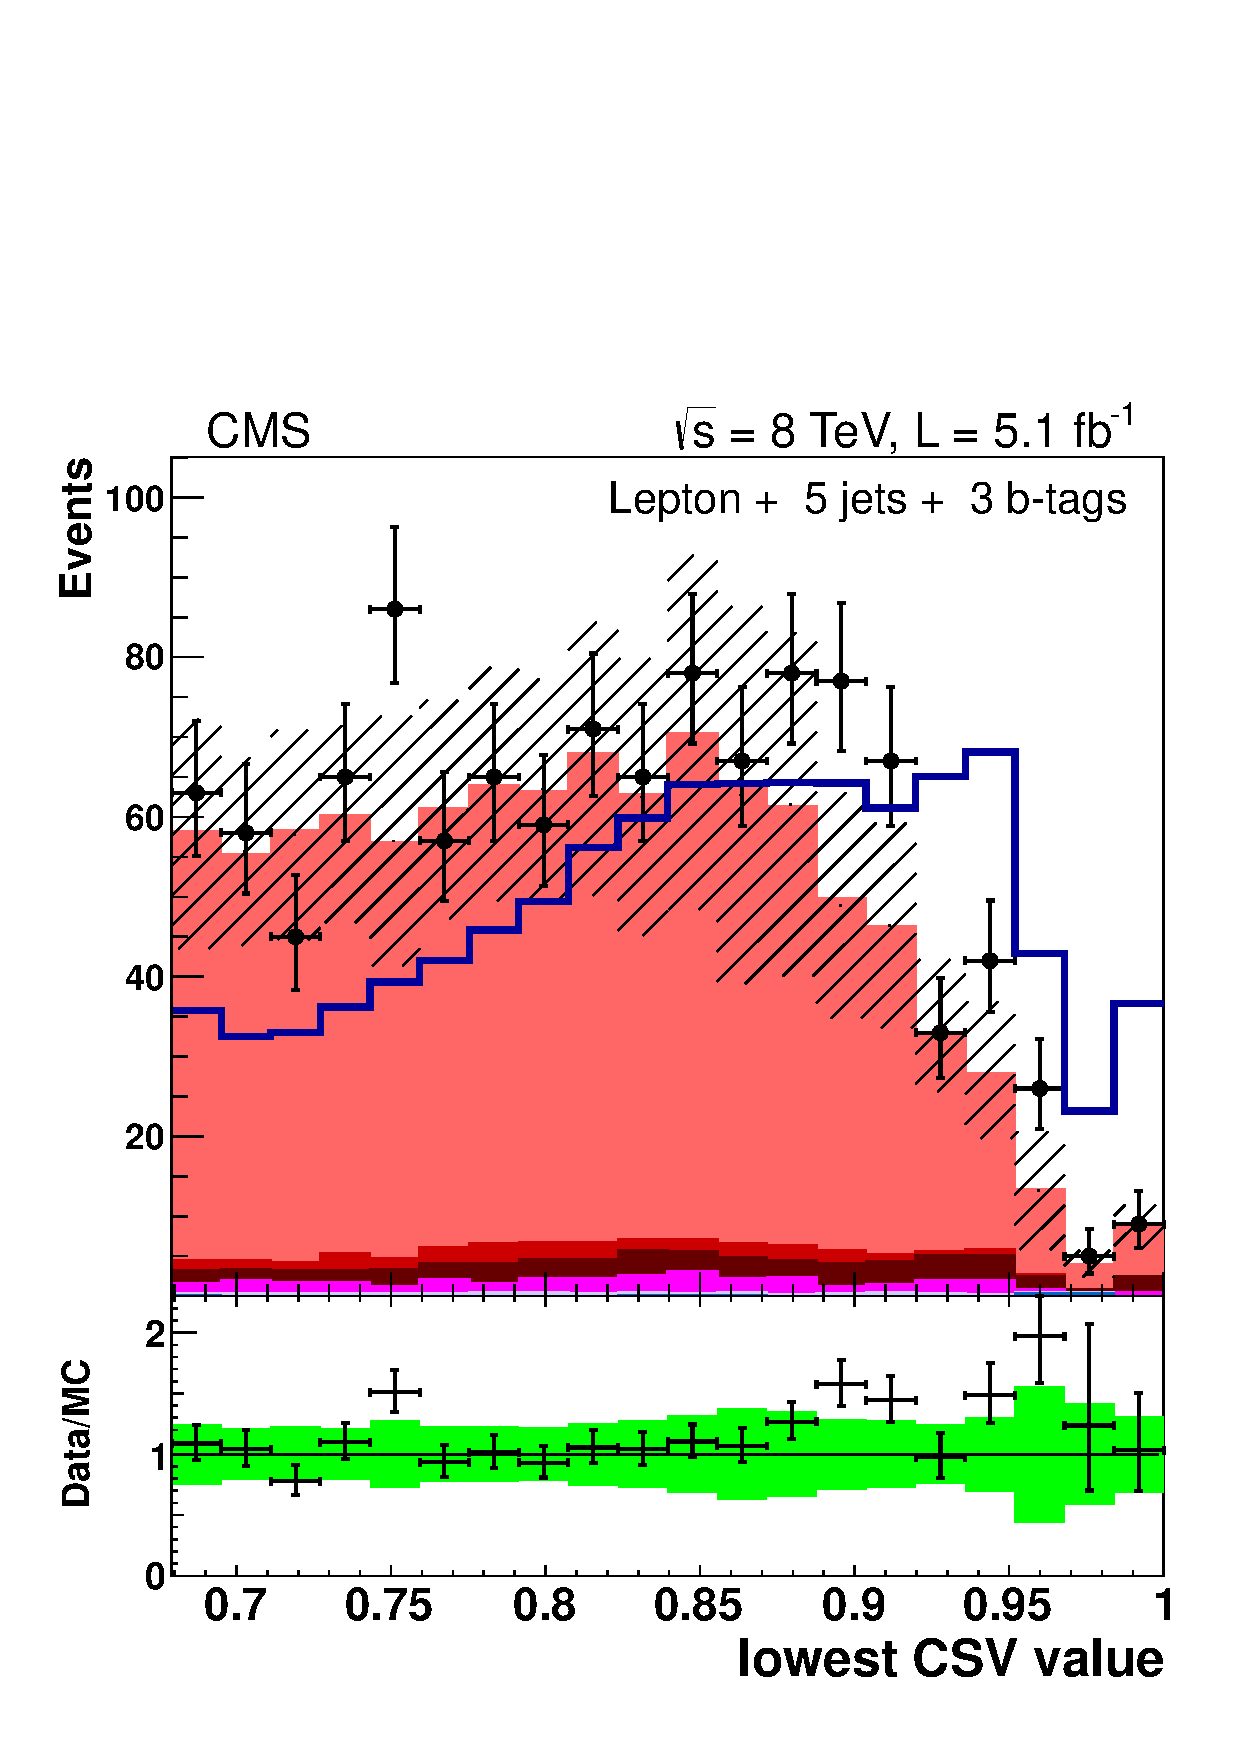
\includegraphics[width=0.31\textwidth]{Figures/Analysis_1_Diagrams/d2MCPlots_lowest_btag_cut5_j5_t3_Combined_HtWgt.pdf}
   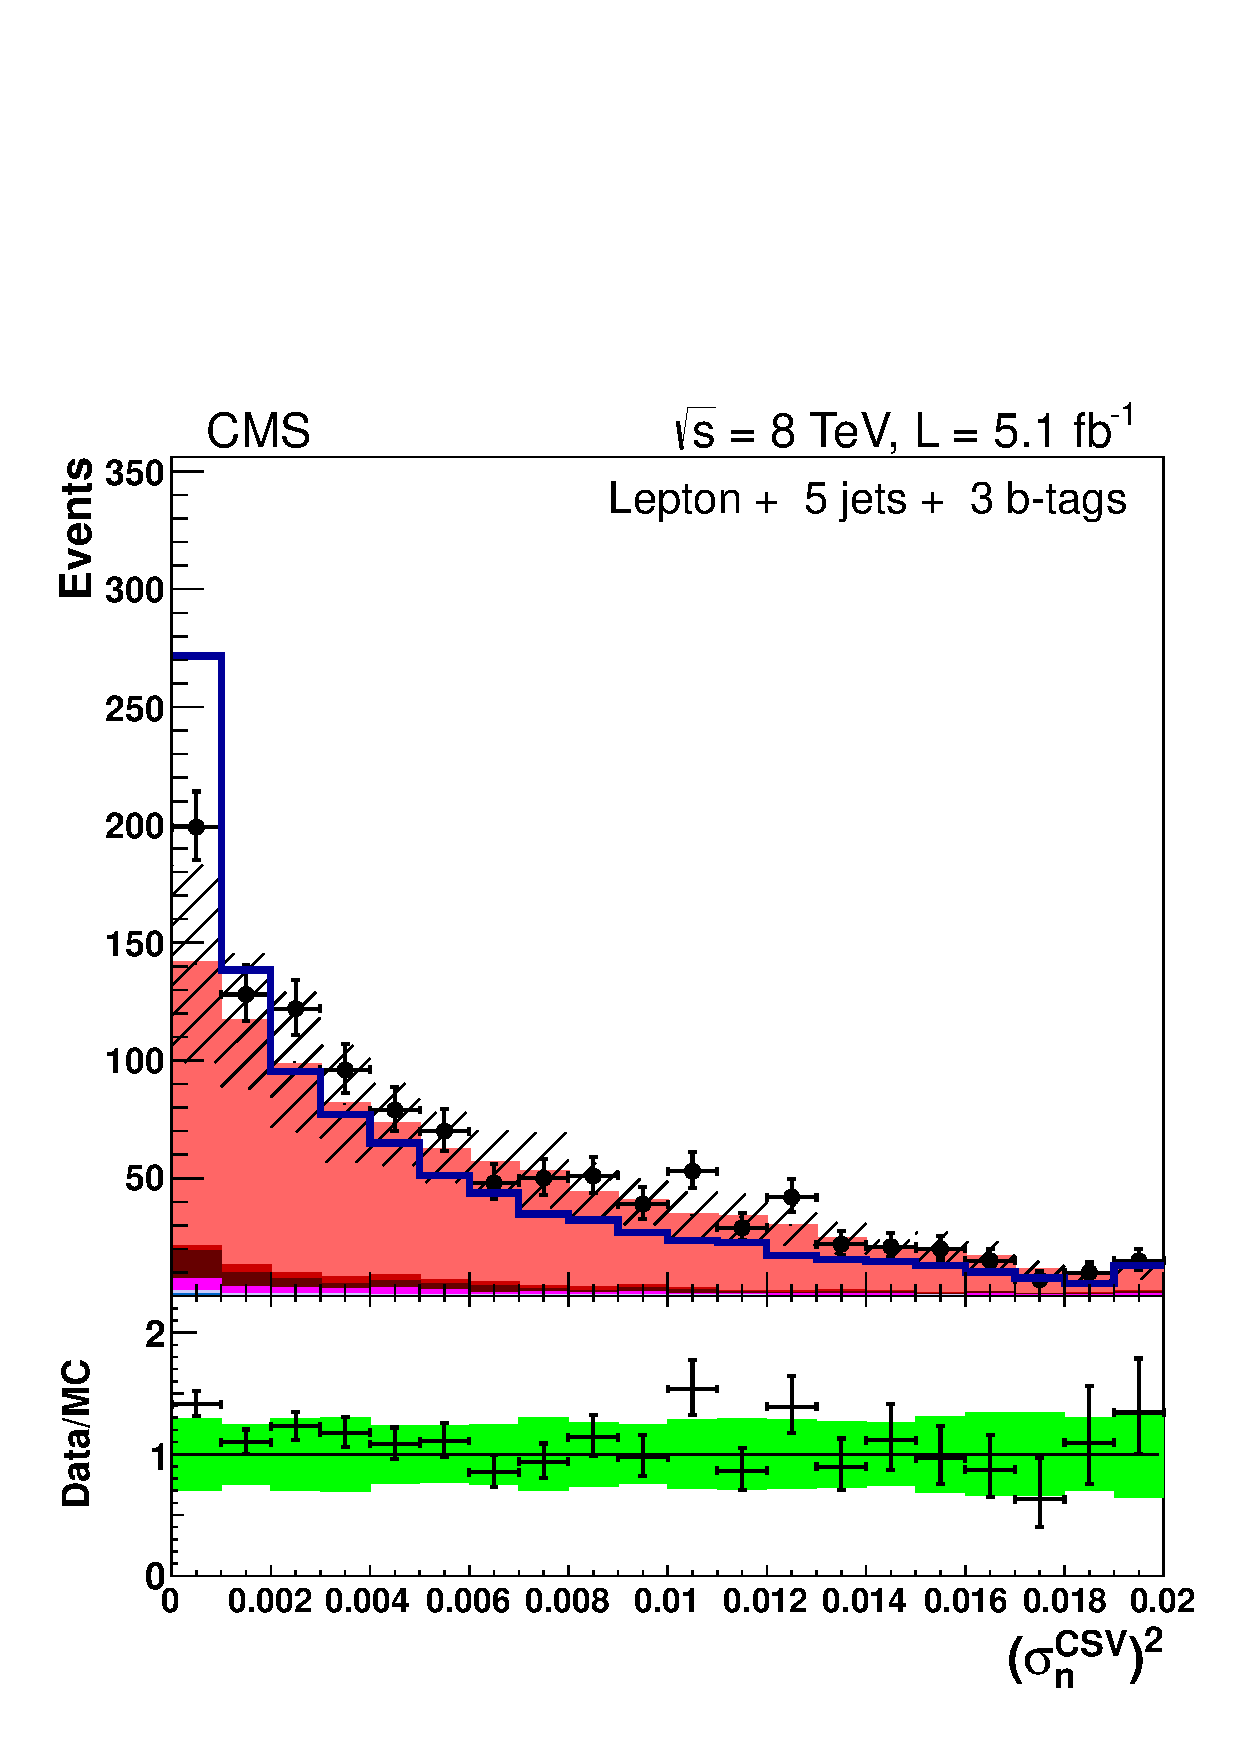
\includegraphics[width=0.31\textwidth]{Figures/Analysis_1_Diagrams/d2MCPlots_dev_from_avg_disc_btags_cut5_j5_t3_Combined_HtWgt.pdf}
   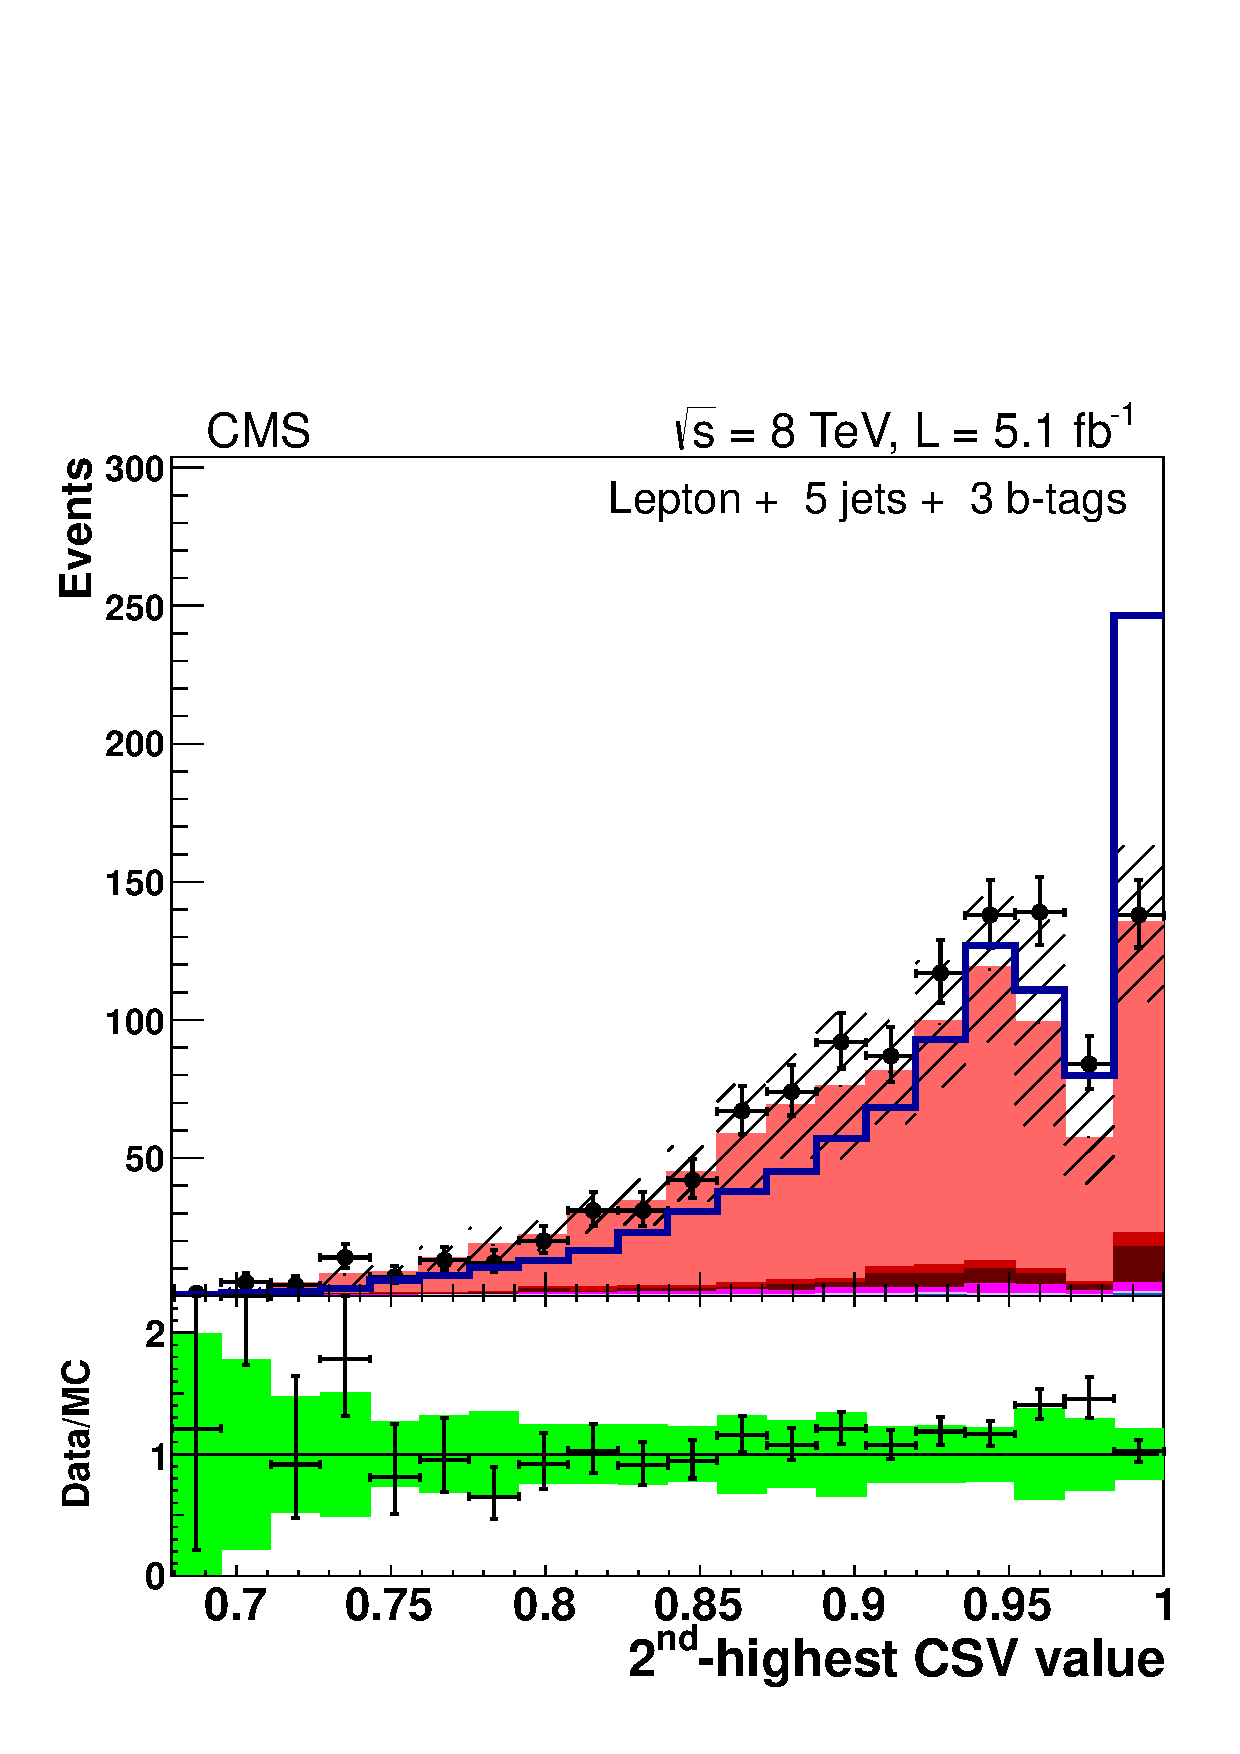
\includegraphics[width=0.31\textwidth]{Figures/Analysis_1_Diagrams/d2MCPlots_second_highest_btag_cut5_j5_t3_Combined_HtWgt.pdf}
   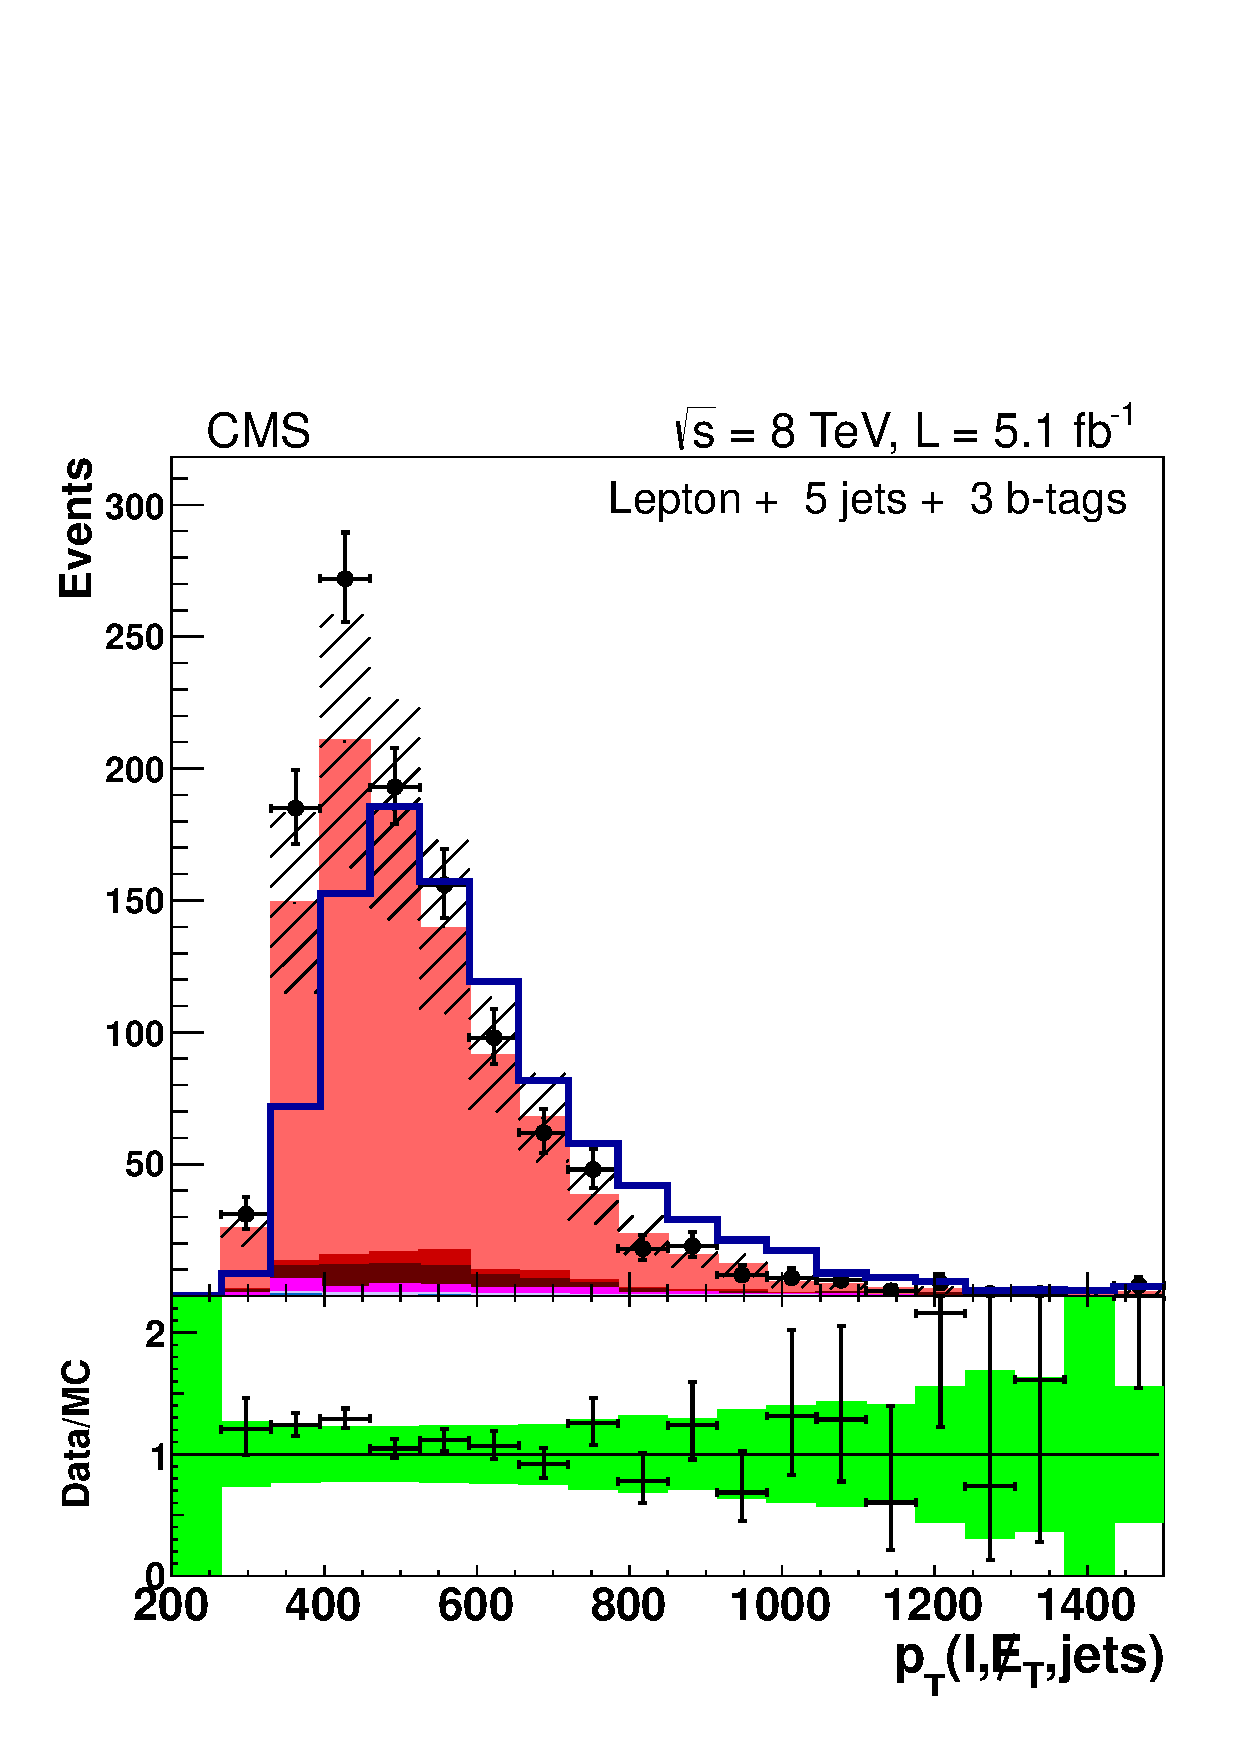
\includegraphics[width=0.31\textwidth]{Figures/Analysis_1_Diagrams/d2MCPlots_all_sum_pt_incl_met_cut5_j5_t3_Combined_HtWgt.pdf}
   \raisebox{0.1\height}{\includegraphics[width=0.25\textwidth]{Figures/Analysis_1_Diagrams/samples_legend_tall_noTTHscale.pdf}}
   \hspace{0.055\textwidth}
   \caption{Distributions of the five ANN input variables with
   rankings 1 through 5, in terms of separation, for the 5~jets +
   3~b-tags category of the lepton+jets channel at $8
   \TeV$. Definitions of the variables are given in the text. The 
   background is normalized to the SM expectation; the
   uncertainty band (shown as a hatched band in the stack plot and a
   green band in the ratio plot) includes statistical and systematic
   uncertainties that affect both the rate and shape of the background
   distributions.  The $\ttH$ signal ($m_{H} = 125 \GeVcc$) is
   normalized to the total background yield, for easier comparison of
   the shapes.} 
   \label{fig:lj_input_5j_3t_part1} \end{center}
\end{figure}

\clearpage

\begin{figure}[hbtp]
 \begin{center}
   \includegraphics[width=0.31\textwidth]{Figures/Analysis_1_Diagrams/d2MCPlots_third_jet_pt_cut5_j5_t3_Combined_HtWgt.pdf}
   \includegraphics[width=0.31\textwidth]{Figures/Analysis_1_Diagrams/d2MCPlots_second_jet_pt_cut5_j5_t3_Combined_HtWgt.pdf}
   \includegraphics[width=0.31\textwidth]{Figures/Analysis_1_Diagrams/d2MCPlots_first_jet_pt_cut5_j5_t3_Combined_HtWgt.pdf}
   \includegraphics[width=0.31\textwidth]{Figures/Analysis_1_Diagrams/d2MCPlots_fourth_jet_pt_cut5_j5_t3_Combined_HtWgt.pdf}
   \includegraphics[width=0.31\textwidth]{Figures/Analysis_1_Diagrams/d2MCPlots_min_dr_tagged_jets_cut5_j5_t3_Combined_HtWgt.pdf}
   \raisebox{0.1\height}{\includegraphics[width=0.25\textwidth]{Figures/Analysis_1_Diagrams/samples_legend_tall_noTTHscale.pdf}}
   \hspace{0.055\textwidth}
   \caption{Distributions of the five ANN input variables with
     rankings 6 through 10, in terms of separation, for the 5~jets +
     3~b-tags category of the lepton+jets channel at $8
     \TeV$. Definitions of the variables are given in the text. The
     background is normalized to the SM expectation; the
     uncertainty band (shown as a hatched band in the stack plot and a
     green band in the ratio plot) includes statistical and systematic
     uncertainties that affect both the rate and shape of the
     background distributions.  The $\ttH$ signal ($m_{H} =
     125 \GeVcc$) is normalized to the total background yield, for
     easier comparison of the
     shapes.}  \label{fig:lj_input_5j_3t_part2} \end{center} 
\end{figure}


%%%%%%%%%%%%%%%%%%%%%%%%%%%%%%%%%%%%%%%%%%%%%%%%%%%%%%%%%%%%%%%
%
%  NN Inputs 6j3t L+J (muon+electron) 8TeV
%
%%%%%%%%%%%%%%%%%%%%%%%%%%%%%%%%%%%%%%%%%%%%%%%%%%%%%%%%%%%%%%%

\clearpage

\begin{figure}[hbtp]
 \begin{center}
   \includegraphics[width=0.31\textwidth]{Figures/Analysis_1_Diagrams/d2MCPlots_avg_dr_tagged_jets_cut6_jge6_t3_Combined_HtWgt.pdf}
   \includegraphics[width=0.31\textwidth]{Figures/Analysis_1_Diagrams/d2MCPlots_avg_untagged_dijet_mass_cut6_jge6_t3_Combined_HtWgt.pdf}
   \includegraphics[width=0.31\textwidth]{Figures/Analysis_1_Diagrams/d2MCPlots_avg_btag_disc_btags_cut6_jge6_t3_Combined_HtWgt.pdf}
   \includegraphics[width=0.31\textwidth]{Figures/Analysis_1_Diagrams/d2MCPlots_dev_from_avg_disc_btags_cut6_jge6_t3_Combined_HtWgt.pdf}
   \includegraphics[width=0.31\textwidth]{Figures/Analysis_1_Diagrams/d2MCPlots_h2_cut6_jge6_t3_Combined_HtWgt.pdf}
   \raisebox{0.1\height}{\includegraphics[width=0.25\textwidth]{Figures/Analysis_1_Diagrams/samples_legend_tall_noTTHscale.pdf}}
   \hspace{0.055\textwidth}
   \caption{Lepton + jets data/MC comparison for the $\ge$6 jets + 3 tag category.  The uncertainty band includes statistical and systematic uncertainties that affect both the rate and shape of the background distributions.}
   \label{fig:lj_input_6j_3t_part1}
 \end{center}
\end{figure}

\clearpage

\begin{figure}[hbtp]
 \begin{center}
   \includegraphics[width=0.31\textwidth]{Figures/Analysis_1_Diagrams/d2MCPlots_h3_cut6_jge6_t3_Combined_HtWgt.pdf}
   \includegraphics[width=0.31\textwidth]{Figures/Analysis_1_Diagrams/d2MCPlots_dijet_mass_of_everything_cut6_jge6_t3_Combined_HtWgt.pdf}
   \includegraphics[width=0.31\textwidth]{Figures/Analysis_1_Diagrams/d2MCPlots_second_highest_btag_cut6_jge6_t3_Combined_HtWgt.pdf}
   \includegraphics[width=0.31\textwidth]{Figures/Analysis_1_Diagrams/d2MCPlots_lowest_btag_cut6_jge6_t3_Combined_HtWgt.pdf}
   \includegraphics[width=0.31\textwidth]{Figures/Analysis_1_Diagrams/d2MCPlots_sphericity_cut6_jge6_t3_Combined_HtWgt.pdf}
   \raisebox{0.1\height}{\includegraphics[width=0.25\textwidth]{Figures/Analysis_1_Diagrams/samples_legend_tall_noTTHscale.pdf}}
   \hspace{0.055\textwidth}
   \caption{Lepton + jets data/MC comparison for the $\ge$6 jets + 3 tag category.  The uncertainty band includes statistical and systematic uncertainties that affect both the rate and shape of the background distributions.}
   \label{fig:lj_input_6j_3t_part2}
 \end{center}
\end{figure}


%%%%%%%%%%%%%%%%%%%%%%%%%%%%%%%%%%%%%%%%%%%%%%%%%%%%%%%%%%%%%%%
%
%  NN Inputs 4j4t L+J (muon+electron) 8TeV
%
%%%%%%%%%%%%%%%%%%%%%%%%%%%%%%%%%%%%%%%%%%%%%%%%%%%%%%%%%%%%%%%

\clearpage

\begin{figure}[hbtp]
 \begin{center}
   \includegraphics[width=0.31\textwidth]{Figures/Analysis_1_Diagrams/d2MCPlots_all_sum_pt_incl_met_cut7_j4_t4_Combined_HtWgt.pdf}
   \includegraphics[width=0.31\textwidth]{Figures/Analysis_1_Diagrams/d2MCPlots_aplanarity_cut7_j4_t4_Combined_HtWgt.pdf}
   \includegraphics[width=0.31\textwidth]{Figures/Analysis_1_Diagrams/d2MCPlots_avg_dr_tagged_jets_cut7_j4_t4_Combined_HtWgt.pdf}
   \includegraphics[width=0.31\textwidth]{Figures/Analysis_1_Diagrams/d2MCPlots_avg_btag_disc_btags_cut7_j4_t4_Combined_HtWgt.pdf}
   \includegraphics[width=0.31\textwidth]{Figures/Analysis_1_Diagrams/d2MCPlots_dev_from_avg_disc_btags_cut7_j4_t4_Combined_HtWgt.pdf}
   \raisebox{0.1\height}{\includegraphics[width=0.25\textwidth]{Figures/Analysis_1_Diagrams/samples_legend_tall_noTTHscale.pdf}}
   \hspace{0.055\textwidth}
   \caption{Lepton + jets data/MC comparison for the 4 jets + 4 tag category.  The uncertainty band includes statistical and systematic uncertainties that affect both the rate and shape of the background distributions.}
   \label{fig:lj_input_4j_4t_part1}
 \end{center}
\end{figure}

\clearpage

\begin{figure}[hbtp]
 \begin{center}
  \includegraphics[width=0.31\textwidth]{Figures/Analysis_1_Diagrams/d2MCPlots_h1_cut7_j4_t4_Combined_HtWgt.pdf}
   \includegraphics[width=0.31\textwidth]{Figures/Analysis_1_Diagrams/d2MCPlots_dijet_mass_of_everything_cut7_j4_t4_Combined_HtWgt.pdf}
   \includegraphics[width=0.31\textwidth]{Figures/Analysis_1_Diagrams/d2MCPlots_first_jet_pt_cut7_j4_t4_Combined_HtWgt.pdf}
   \includegraphics[width=0.31\textwidth]{Figures/Analysis_1_Diagrams/d2MCPlots_second_highest_btag_cut7_j4_t4_Combined_HtWgt.pdf}
   \includegraphics[width=0.31\textwidth]{Figures/Analysis_1_Diagrams/d2MCPlots_lowest_btag_cut7_j4_t4_Combined_HtWgt.pdf}
   \raisebox{0.1\height}{\includegraphics[width=0.25\textwidth]{Figures/Analysis_1_Diagrams/samples_legend_tall_noTTHscale.pdf}}
   \hspace{0.055\textwidth}
   \caption{Lepton + jets data/MC comparison for the 4 jets + 4 tag category.  The uncertainty band includes statistical and systematic uncertainties that affect both the rate and shape of the background distributions.}
   \label{fig:lj_input_4j_4t_part2}
 \end{center}
\end{figure}


%%%%%%%%%%%%%%%%%%%%%%%%%%%%%%%%%%%%%%%%%%%%%%%%%%%%%%%%%%%%%%%
%
%  NN Inputs 5j4t L+J (muon+electron) 8TeV
%
%%%%%%%%%%%%%%%%%%%%%%%%%%%%%%%%%%%%%%%%%%%%%%%%%%%%%%%%%%%%%%%

\clearpage

\begin{figure}[hbtp]
 \begin{center}
   \includegraphics[width=0.31\textwidth]{Figures/Analysis_1_Diagrams/d2MCPlots_all_sum_pt_incl_met_cut8_j5_tge4_Combined_HtWgt.pdf}
   \includegraphics[width=0.31\textwidth]{Figures/Analysis_1_Diagrams/d2MCPlots_avg_dr_tagged_jets_cut8_j5_tge4_Combined_HtWgt.pdf}
   \includegraphics[width=0.31\textwidth]{Figures/Analysis_1_Diagrams/d2MCPlots_avg_btag_disc_btags_cut8_j5_tge4_Combined_HtWgt.pdf}
   \includegraphics[width=0.31\textwidth]{Figures/Analysis_1_Diagrams/d2MCPlots_dev_from_avg_disc_btags_cut8_j5_tge4_Combined_HtWgt.pdf}
   \includegraphics[width=0.31\textwidth]{Figures/Analysis_1_Diagrams/d2MCPlots_first_highest_btag_cut8_j5_tge4_Combined_HtWgt.pdf}
   \raisebox{0.1\height}{\includegraphics[width=0.25\textwidth]{Figures/Analysis_1_Diagrams/samples_legend_tall_noTTHscale.pdf}}
   \hspace{0.055\textwidth}
   \caption{Lepton + jets data/MC comparison for the 5 jets + 4 tag category.  The uncertainty band includes statistical and systematic uncertainties that affect both the rate and shape of the background distributions.}
   \label{fig:lj_input_5j_4t_part1}
 \end{center}
\end{figure}

\clearpage

\begin{figure}[hbtp]
 \begin{center}
   \includegraphics[width=0.31\textwidth]{Figures/Analysis_1_Diagrams/d2MCPlots_second_highest_btag_cut8_j5_tge4_Combined_HtWgt.pdf}
   \includegraphics[width=0.31\textwidth]{Figures/Analysis_1_Diagrams/d2MCPlots_third_jet_pt_cut8_j5_tge4_Combined_HtWgt.pdf}
   \includegraphics[width=0.31\textwidth]{Figures/Analysis_1_Diagrams/d2MCPlots_fourth_jet_pt_cut8_j5_tge4_Combined_HtWgt.pdf}
   \includegraphics[width=0.31\textwidth]{Figures/Analysis_1_Diagrams/d2MCPlots_lowest_btag_cut8_j5_tge4_Combined_HtWgt.pdf}
   \includegraphics[width=0.31\textwidth]{Figures/Analysis_1_Diagrams/d2MCPlots_dr_between_lep_and_closest_jet_cut8_j5_tge4_Combined_HtWgt.pdf}
   \raisebox{0.1\height}{\includegraphics[width=0.25\textwidth]{Figures/Analysis_1_Diagrams/samples_legend_tall_noTTHscale.pdf}}
   \hspace{0.055\textwidth}
   \caption{Lepton + jets data/MC comparison for the 5 jets + 4 tag category.  The uncertainty band includes statistical and systematic uncertainties that affect both the rate and shape of the background distributions.}
   \label{fig:lj_input_5j_4t_part2}
 \end{center}
\end{figure}

%%%%%%%%%%%%%%%%%%%%%%%%%%%%%%%%%%%%%%%%%%%%%%%%%%%%%%%%%%%%%%%
%
%  NN Inputs 6j4t L+J (muon+electron) 8TeV
%
%%%%%%%%%%%%%%%%%%%%%%%%%%%%%%%%%%%%%%%%%%%%%%%%%%%%%%%%%%%%%%%

\clearpage

\begin{figure}[hbtp]
 \begin{center}
   \includegraphics[width=0.31\textwidth]{Figures/Analysis_1_Diagrams/d2MCPlots_avg_dr_tagged_jets_cut9_jge6_tge4_Combined_HtWgt.pdf}
   \includegraphics[width=0.31\textwidth]{Figures/Analysis_1_Diagrams/d2MCPlots_sphericity_cut9_jge6_tge4_Combined_HtWgt.pdf}
   \includegraphics[width=0.31\textwidth]{Figures/Analysis_1_Diagrams/d2MCPlots_min_dr_tagged_jets_cut9_jge6_tge4_Combined_HtWgt.pdf}
   \includegraphics[width=0.31\textwidth]{Figures/Analysis_1_Diagrams/d2MCPlots_avg_btag_disc_btags_cut9_jge6_tge4_Combined_HtWgt.pdf}
   \includegraphics[width=0.31\textwidth]{Figures/Analysis_1_Diagrams/d2MCPlots_second_highest_btag_cut9_jge6_tge4_Combined_HtWgt.pdf}
   \raisebox{0.1\height}{\includegraphics[width=0.25\textwidth]{Figures/Analysis_1_Diagrams/samples_legend_tall_noTTHscale.pdf}}
   \hspace{0.055\textwidth}
   \caption{Lepton + jets data/MC comparison for the $\ge$ 6 jets + 4 tag category.  The uncertainty band includes statistical and systematic uncertainties that affect both the rate and shape of the background distributions.}
   \label{fig:lj_input_6j_4t_part1}
 \end{center}
\end{figure}

\clearpage

\begin{figure}[hbtp]
 \begin{center}
   \includegraphics[width=0.31\textwidth]{Figures/Analysis_1_Diagrams/d2MCPlots_h2_cut9_jge6_tge4_Combined_HtWgt.pdf}
   \includegraphics[width=0.31\textwidth]{Figures/Analysis_1_Diagrams/d2MCPlots_lowest_btag_cut9_jge6_tge4_Combined_HtWgt.pdf}
   \includegraphics[width=0.31\textwidth]{Figures/Analysis_1_Diagrams/d2MCPlots_closest_tagged_dijet_mass_cut9_jge6_tge4_Combined_HtWgt.pdf}
   \includegraphics[width=0.31\textwidth]{Figures/Analysis_1_Diagrams/d2MCPlots_h3_cut9_jge6_tge4_Combined_HtWgt.pdf}
   \includegraphics[width=0.31\textwidth]{Figures/Analysis_1_Diagrams/d2MCPlots_dijet_mass_of_everything_cut9_jge6_tge4_Combined_HtWgt.pdf}
   \includegraphics[width=0.31\textwidth]{Figures/Analysis_1_Diagrams/d2MCPlots_best_higgs_mass_cut9_jge6_tge4_Combined_HtWgt.pdf}
   \raisebox{0.1\height}{\includegraphics[width=0.8\textwidth]{Figures/Analysis_1_Diagrams/samples_legend_wide_noTTHscale.pdf}}
   \hspace{0.055\textwidth}
   \caption{Lepton + jets data/MC comparison for the $\ge$ 6 jets + 4 tag category.  The uncertainty band includes statistical and systematic uncertainties that affect both the rate and shape of the background distributions.}
   \label{fig:lj_input_6j_4t_part2}
 \end{center}
\end{figure}


\subsection{MVA Output, Data to Monte Carlo Comparisons}
\label{mva_input_vars_data_to_mc_overview}

\par Data to Monte Carlo comparisons for the CFMlpANN output can be
seen on figure \ref{fig:lj_ANNoutput_8TeV}.  In the plots, the signal
shape has been multiplied by a factor of 30 in order to make its shape
visible, and in order to gauge a scale of the expected size of signal
to background in each jet/tag category.  

%%%%%%%%%%%%%%%%%%%%%%%%%%%%%%%%%%%%%%%%%%%%%%%%%%%%%%%%%%%%%%%
%
%  NN Output all-categories L+J (muon+electron) 8TeV
%
%%%%%%%%%%%%%%%%%%%%%%%%%%%%%%%%%%%%%%%%%%%%%%%%%%%%%%%%%%%%%%%

\begin{figure}{h}
    \centering
    \begin{subfigure}[h]{0.31\textwidth}
        \includegraphics[width=\textwidth]{Figures/Analysis_1_Diagrams/d2MCPlots_CFMlpANN_cut3_jge6_t2_Combined_HtWgt.pdf}
        \caption{$\ge$6 jets, 2 $b$-tags}\label{lj_ANNoutput_8TeV_1}
      \end{subfigure}
      ~ %add desired spacing between images, e. g. ~, \quad, \qquad, \hfill etc.
      % (or a blank line to force the subfigure onto a new line)
      \begin{subfigure}[h]{0.31\textwidth}
        \includegraphics[width=\textwidth]{Figures/Analysis_1_Diagrams/d2MCPlots_CFMlpANN_cut4_j4_t3_Combined_HtWgt.pdf}
        \caption{4 jets, 3 $b$-tags}\label{lj_ANNoutput_8TeV_2}
      \end{subfigure}
      ~ %add desired spacing between images, e. g. ~, \quad, \qquad, \hfill etc.
      % (or a blank line to force the subfigure onto a new line)
      \begin{subfigure}[h]{0.31\textwidth}
        \includegraphics[width=\textwidth]{Figures/Analysis_1_Diagrams/d2MCPlots_CFMlpANN_cut5_j5_t3_Combined_HtWgt.pdf}
        \caption{5 jets, 3 $b$-tags}\label{lj_ANNoutput_8TeV_3}
      \end{subfigure}
      ~ %add desired spacing between images, e. g. ~, \quad, \qquad, \hfill etc.
      % (or a blank line to force the subfigure onto a new line)
      \begin{subfigure}[h]{0.31\textwidth}
        \includegraphics[width=\textwidth]{Figures/Analysis_1_Diagrams/d2MCPlots_CFMlpANN_cut6_jge6_t3_Combined_HtWgt.pdf}
        \caption{$\ge$6 jets, 3 $b$-tags}\label{lj_ANNoutput_8TeV_4}
      \end{subfigure}
      ~ %add desired spacing between images, e. g. ~, \quad, \qquad, \hfill etc.
      % (or a blank line to force the subfigure onto a new line)
      \begin{subfigure}[h]{0.31\textwidth}
        \includegraphics[width=\textwidth]{Figures/Analysis_1_Diagrams/d2MCPlots_CFMlpANN_cut7_j4_t4_Combined_HtWgt.pdf}
        \caption{4 jets, 4 $b$-tags}\label{lj_ANNoutput_8TeV_5}
      \end{subfigure}
      ~ %add desired spacing between images, e. g. ~, \quad, \qquad, \hfill etc.
      % (or a blank line to force the subfigure onto a new line)
      \begin{subfigure}[h]{0.31\textwidth}
        \includegraphics[width=\textwidth]{Figures/Analysis_1_Diagrams/d2MCPlots_CFMlpANN_cut8_j5_tge4_Combined_HtWgt.pdf}
        \caption{5 jets, $\ge$4 $b$-tags}\label{lj_ANNoutput_8TeV_6}
      \end{subfigure}
      ~ %add desired spacing between images, e. g. ~, \quad, \qquad, \hfill etc.
      % (or a blank line to force the subfigure onto a new line)
      \begin{subfigure}[h]{0.31\textwidth}
        \includegraphics[width=\textwidth]{Figures/Analysis_1_Diagrams/d2MCPlots_CFMlpANN_cut9_jge6_tge4_Combined_HtWgt.pdf}
        \caption{$\ge$6 jets, $\ge$4 $b$-tags}\label{lj_ANNoutput_8TeV_7}
      \end{subfigure}
      ~ %add desired spacing between images, e. g. ~, \quad, \qquad, \hfill etc.
      % (or a blank line to force the subfigure onto a new line)
      \begin{subfigure}[h]{0.25\textwidth}
        \includegraphics[width=\textwidth]{Figures/Analysis_1_Diagrams/samples_legend_tall_noTTHscale.pdf}
        \caption{Legend}\label{lj_ANNoutput_8TeV_8_leg}
      \end{subfigure}
      \caption{The distributions of the CFMlpANN output for lepton+jets
     events at $8 \TeV$ in the various analysis categories.
     Background-like events have a
     low CFMlpANN output value. Signal-like events have a high
     CFMlpANN output value.  The background is normalized to the SM expectation; 
     the uncertainty (shown as a
     hatched band in the stack plot and a green band in the ratio
     plot) includes statistical and systematic uncertainties that
     affect both the rate and shape of the background distributions.
     The $\ttH$ signal ($m_{H} = 125 \GeVcc$) is normalized to
     30 $\times$ SM expectation.}  \label{fig:lj_ANNoutput_8TeV}
\end{figure}


\section{Systematic Uncertainties}
\label{systematics_overview}

\par There are three types of systematic effects considered in this
analysis: those that affect only the rates of signal or background
processes, those that affect only the shapes of the CFMlpANN
discriminants for signal or background processes, and those that
affect both the rate and the shape.  In the last case, the rate and
shape effects are treated simultaneously so that they are considered
completely correlated.  Unless otherwise noted, all of the
uncertainties listed here apply equally to signal and background and
are treated as 100\%  correlated between the two.  Below is a list of
systematic effects considered for this analysis:

\begin{table}[hbtp] \small
\centering
\caption{Summary of the systematic uncertainties considered on the inputs to the limit calculation.  Except where noted, each row in this table will be treated as a single, independent nuisance parameter.} 
\label{tab:syst}
\begin{tabular}{|l|c|c|l|}
\hline\hline
Source & Rate Uncertainty & Shape & Remarks \\
\hline
Luminosity ($8 \TeV$) & 2.2\% & No & All signal and backgrounds \\
Lepton ID/Trig & 4\% & No & All signal and backgrounds \\
Pileup & 1\% & No & All signal and backgrounds \\
Additional Pileup Corr. & -- & Yes & All signal and backgrounds \\
Jet Energy Resolution & 1.5\% & No & All signal and backgrounds \\
Jet Energy Scale & 0-60\% & Yes & All signal and backgrounds \\
b-Tag SF ($b/c$) & 0-33.6\% & Yes & All signal and backgrounds \\
b-Tag SF (mistag) & 0-23.5\% & Yes & All signal and backgrounds \\
MC Statistics & -- & Yes & All backgrounds \\ 
\hline
PDF ($gg$) & 9\% & No & For $gg$ initiated processes ($\ttbar$, $\ttbar$Z, $\ttH$) \\
PDF ($q\bar{q}$) & 4.2-7\% & No & For $q\bar{q}$ initiated processes ($\ttbar W$, $W$, $Z$). \\
PDF ($qg$) & 4.6\% & No & For $qg$ initiated processes (single top) \\
\hline
QCD Scale ($\ttH$) & 15\% & No & For NLO $t\bar{t}H$ prediction \\
QCD Scale ($\ttbar$) & 2-12\% & No & For NLO $t\bar{t}$ and single top predictions \\
QCD Scale (V) & 1.2-1.3\% & No & For NNLO $W$ and $Z$ prediction \\
QCD Scale (VV) & 3.5\% & No & For NLO diboson prediction \\
\hline
Madgraph Scale ($\ttbar$) & 0-20\% & Yes & $\ttbar+$jets$/b\bar{b}/c\bar{c}$ uncorrelated. Varies by jet bin.\\
Madgraph Scale (V) & 20-60\% & No & Varies by jet bin. \\
\hline
$\ttbar + \bbbar$ & 50\% & No & Only $t\bar{t} + b\bar{b}$. \\
\hline\hline
\end{tabular}
\end{table}


\begin{description}
  \item[Jet Energy Scale (JES):]  THe Jet Energy Scale systematic is
    based on the uncertainy on the L1, L2, L3, and L2L3 residual
    corrections to the reconstructed jet energy, as described in
    section \ref{jet_selection_overview}.  To evaluate the effect on
    the CFMlpANN output, the jet energy scale is shifted by one
    standard deviation up and down using the standard JetMET
    procedure~\cite{JESJetMET}.  For each variation, the jet energies 
    are recalulated, allowing for new jets to pass the selection where
    once they failed, or fail the selection where once they passed,
    resulting in a migration of events across jet/tag cateogries.
    Finally, the CFMlpANN response is recalculated, and the effect for
    signal and the \ttjets background is shown in figure
    \ref{fig:JESShift}. 

\begin{figure}[h]
  \centering
   \includegraphics[width=0.45\textwidth]{Figures/Analysis_1_Diagrams/SystPlot_CMS_scale_j_ttH120_ljets_jge6_tge4.pdf}
   \includegraphics[width=0.45\textwidth]{Figures/Analysis_1_Diagrams/SystPlot_CMS_scale_j_ttbar_ljets_jge6_tge4.pdf}
   \caption{ Comparison of the MVA discriminator for JES shift upwards
     (red) and downwards (blue) relative to the nominal (black) shape
     for the $t\bar{t}H(120)$ signal (left) and the main background sample
     $t\bar{t}+$ light flavor (right).  The plots shown are from the
     $\ge$6 jet $\ge$4 tag category in the lepton+jets channel.  All plots are normalized to unit area.}\label{fig:JESShift}
\end{figure}


\begin{table}[h] 
  \centering 
   \begin{tabular}{|c|c|c|c|c|c|} \hline 
\multicolumn{4}{|c|}{JES systematic yield change} \\ \hline
\multicolumn{2}{|c|}{ } & \multicolumn{2}{|c|}{lepton+jets} \\ \hline
sys & shift & $t\bar{t}H(120)$ & $t\bar{t}$  \\ \hline 
\multirow{2}{*}{JES} & up  & +8.6\% & +12.1\% \\
                     & down & -8.4\% & -7.3\% \\ \hline
  \end{tabular} 
  \caption{Relative yield change due to JES shift up/down for the
    $\ge$ 6 jets + $\ge$ 4 tags category in the
     lepton+jets channel.}
  \label{tab:JESShift}
\end{table} 

\item[Jet Energy Resolution (JER):]  The jet $p_T$ resolution in MC
  differs from that observed in data by approximately 10\% in a $\eta$
  dependent way, as described in table \ref{tab:JERtab}, as per the
  recommendations of the JetMET group~\cite{JERJetMET}.  The value of
  the jet $p_T$  is adjusted according to the formula:
\begin{equation}\label{eq:jer_formula}
p_T^{\prime} = \max{\left[0,p_T^{gen}+c(p_T^{reco}-p_T^{gen})\right]}
\end{equation}

  The correction factor $c$ is taken from table \ref{tab:JERtab}.  To
  assess the effect of the systematic uncertainty on the JER, the
  value of $c$ is shifted up and down by standard deviation, the JER
  correction is applied to the jets using this new $c$ value, and the
  event rates and ANN shapes are recalculated.  The effect of the JER
  on the shape variation is negligible, so it is treated as a
  rate-only effect in limit setting.  


\item[$b$-tag Scale Factor:] The uncertainty in the $b$-tagging
    scale factor is assessed according to the prescriptions developed
    by the BTag POG~\cite{btagSF}.  Each per-jet $b$-tag scale factor
    is shifted up or down by its uncertainty, and the new CSV output
    value corresponding to that uncertainty is recalculated  This new
    CSV value is used to determine both the number of tags associated with
    that systematic and the new shape of
    variables that use the CSV output, such as the average CSV value
    for $b$-tagged jets.  This uncertainty effects both rate and shape estimates.  
    The effects of the $b$-tag scale factors on the ANN shape and
    event yields are summarized in Fig.~\ref{fig:btagSFShift} and
    Table~\ref{tab:btagSFShift} respectively. 

\begin{figure}[hbtp]
 \begin{center}
   \includegraphics[width=0.35\textwidth]{Figures/Analysis_1_Diagrams/SystPlot_CMS_eff_b_ttH120_ljets_jge6_tge4}
   \includegraphics[width=0.35\textwidth]{Figures/Analysis_1_Diagrams/SystPlot_CMS_eff_b_ttbar_ljets_jge6_tge4}
   \includegraphics[width=0.35\textwidth]{Figures/Analysis_1_Diagrams/SystPlot_CMS_fake_b_ttH120_ljets_jge6_tge4}
   \includegraphics[width=0.35\textwidth]{Figures/Analysis_1_Diagrams/SystPlot_CMS_fake_b_ttbar_ljets_jge6_tge4}
   \caption{ Comparison of the MVA discriminator for  $b$-tag scale factor shift upwards
     (red) and downwards (blue) relative to the nominal (black) shape
     for the $t\bar{t}H(120)$ signal (left) and the main background sample
     $t\bar{t}~+$ light flavor (right).  The plots are from the $\ge$6
     jets + $\ge$4 tags category in the lepton+jets channel.  All
     plots are normalized to unit area.}\label{fig:btagSFShift}
 \end{center}
\end{figure}


 \begin{table}[hbtp] 
   \centering 
   \begin{tabular}{|c|c|c|c|} \hline 
     \multicolumn{4}{|c|}{$b$-tag systematic yield change} \\ \hline
     \multicolumn{2}{|c}{ } & \multicolumn{2}{|c|}{lepton+jets} \\ \hline
     sys & shift & $t\bar{t}H(120)$ & $t\bar{t}$  \\ \hline 
     \multirow{2}{*}{heavy flavor SF} & up     & +14.9\%  & +23.7\% \\
                            & down & -15.3\%  & -16.0\% \\ \hline
     \multirow{2}{*}{light flavor SF} & up     & +0.7\%  & +5.7\% \\
                            & down & -1.1\%  & -4.2\% \\ \hline
   \end{tabular} 
   \caption{Relative yield change due to $b$-tag scale factor shift up/down for the
     $\ge$6 jets + $\ge$4 tags category in the  lepton+jets channel.}
   \label{tab:btagSFShift}
 \end{table} 


  \item[Lepton ID and Trigger Scale Factors:] As discussed previously,
    an uncertainty of 4\% covers variations of the combined trigger,
    ID, and isolation scale factor.  

  \item[Pileup Reweighting:]  The uncertainty on the pileup
    reweighting comes from changing the minimum bias cross section
    used to calculate the pileup reweighting by $\pm$7\% from the
    default value of 69.4~mb.  The pileup reweighting is calculated
    using the shifted cross sections and the new weights are applied
    to determine the uncertainty on both the rate and shapes. Since
    the effect of the pileup on the shape variation is negligible, the
    effects of pileup are accounted through a rate-only uncertainty
    for the limit calculations. 

    \item[Additional Pileup Correction] The uncertainty associated
      with the additional pileup correction, described in section
      \ref{additional_pileup_reweight_overview}, is applied as a pure
      shape uncertainty to all processes.  Fig.~\ref{fig:addPUCorr} shows
      the effects of the additional pileup correct uncertainty on the
      CFMlpANN shape. 

\begin{figure}[hbtp]
 \begin{center}
   \includegraphics[width=0.35\textwidth]{Figures/Analysis_1_Diagrams/SystPlot_rwt_ttH120_ljets_jge6_tge4.pdf}
   \includegraphics[width=0.35\textwidth]{Figures/Analysis_1_Diagrams/SystPlot_rwt_ttbar_ljets_jge6_tge4.pdf}
  \caption{Comparison of the MVA discriminator for  additional PU correction systematic upwards
     (red) and downwards (blue) relative to the nominal (black) shape
     for the $t\bar{t}H(120)$ signal (left) and the main background sample
     $t\bar{t}\ +$ light flavor (right).  The plots are from the
     $\ge$6 jets + $\ge$4 tags category in the lepton+jets channel.
     All plots are normalized to unit area.}\label{fig:addPUCorr}
 \end{center}
\end{figure}

  \item[Cross Sections:] The expectation for signal and background
    yields are derived from theoretical predictions of at least NLO
    accuracy.  Uncertainties affecting these normalizations are
    summarized in table~\ref{tab:xsUncertainty}.  Where appropriate,
    factors contributing to these uncertainties that are common to
    multiple processes are treated as 100\% correlated.  Note that for
    the $t\bar{t}+$jets (including $t\bar{t}+b\bar{b}$ and
    $t\bar{t}+c\bar{c}$ processes, as well as the $V+$jets processes,
    there is an additional uncertainty coming from the scale choice in
    Madgraph that effects these channels in a jet-bin specific way.
    This uncertainty is not included in the
    table~\ref{tab:xsUncertainty}, but is detailed in the next point.  

\begin{table}[hbtp]
\centering
\begin{tabular}{|l|c|c|c|c|c|c|c|c|}
\hline\hline
\multirow{2}{*}{Process} & \multicolumn{3}{c|}{pdf} & \multicolumn{4}{c|}{QCD Scale} \\
\cline{2-8}
                & $gg$  & $q\bar{b}$ & $qg$  & $t\bar{t}$ & $V$   & $VV$  & $t\bar{t}H$\\
\hline
$t\bar{t}H$     & 9\%   &            &       &            &       &       & 12.5\% \\
\hline
$t\bar{t}+$jets & 9\%   &            &       & 12\%       &       &       &      \\
\hline
$t\bar{t}+W$    &       & 7\%        &       & 15\%       &       &       &  \\
\hline
$t\bar{t}+Z$    & 9\%   &            &       & 15\%        &       &       &  \\
\hline
Single top      &       &            & 4.6\% &  2\%       &       &       &    \\
\hline
$W+$jets        &       & 4.8\%      &       &            & 1.3\% &       &   \\
\hline
$Z+$jets        &       & 4.2\%      &       &            & 1.2\% &       &  \\
\hline
Dibosons        &       &            &       &            &       & 3.5\% &  \\
\hline\hline
\end{tabular}
\caption{Cross section uncertainties used for the limit settings.  Each column in the table is an independent source of uncertainty, except for the last column which represents uncertainties uncorrelated with any others.  Uncertainties in the same column for two different processes (different rows) are completely correlated.}
\label{tab:xsUncertainty}
\end{table}

 \item[Luminosity:] The uncertainty on the luminosity estimate is 2.2\%.  This affects all rates.

 \item[Madgraph $Q^2$ Uncertainty:] Although that backgrounds are
   normalizaed using NLO accurate theoretical caluclations, these are
   only applicable to inclusive distributions.  To extrapolate these
   inclusive predictions to exclusive rates in particular jet bins
   requires the use of a Monte Carlo sample.  The {\sc
     Madgraph} generator is used at the matrix element level and
   includes tree-level calculations for processes with multiple
   additional jets, matched to the {\sc Pythia} parton shower to model
   additional soft and colinear radiation.  Since the {\sc Madgraph +
     Pythia} is tree-level, the choice of the renormalizations and
   factorizations scales in this calculation has a significant
   impact.  To include the effects of this uncertainty, the
   factorization and renomaralization scales are varied by a factor of
   two.  The ideal way to study this effect would be to generate
  dedicated samples with the varied scale choice, however the required
  statistics to get a precise determination of the systematic effect
  is computationally prohibitive.  Therefore, as an alternative, we
  reweight the amples, dividing by the appropriate power of $\alpha_s$
  and the $pdf$ values at the original scale, and multiplying by the
  values at the new scale choice.  This reweighting procedure is supported by
  the CMS Monte Carlo Generators group, and has been validated against
  dedicated scale-varied samples and has been shown to produce consistent
  results~\cite{Q2-REWEIGHT-PRESENTATION}.  This reweighting procedure
  provides both a rate and a shape uncertainty, separately for
  $t\bar{t}+$light flavor, $t\bar{t}+c\bar{c}$, and
  $t\bar{t}+b\bar{b}$ components of the $t\bar{t}$ sample.
  Figure~\ref{fig:Q2plots} shows the shape and rate variations for
  selected event categories.  To prevent the strength of the
  $t\bar{t}+$jets constraint from overconstraining the
  $t\bar{t}+b\bar{b}$ and $t\bar{t}+c\bar{c}$ components, we allow the
  Madgraph scale to vary independently for these three components. 

\begin{figure}[hbtp]
 \begin{center}
   \includegraphics[width=0.3\textwidth]{Figures/Analysis_1_Diagrams/Q2Plot_ttbar_CFMlpANN_ljets_j5_t3_Q2scale_ttH_ttbar}
   \includegraphics[width=0.3\textwidth]{Figures/Analysis_1_Diagrams/Q2Plot_ttbarPlusCCbar_CFMlpANN_ljets_j5_t3_Q2scale_ttH_ttbar_cc}
   \includegraphics[width=0.3\textwidth]{Figures/Analysis_1_Diagrams/Q2Plot_ttbarPlusBBbar_CFMlpANN_ljets_j5_t3_Q2scale_ttH_ttbar_bb}
   \includegraphics[width=0.3\textwidth]{Figures/Analysis_1_Diagrams/Q2Plot_ttbar_CFMlpANN_ljets_jge6_tge4_Q2scale_ttH_ttbar}
   \includegraphics[width=0.3\textwidth]{Figures/Analysis_1_Diagrams/Q2Plot_ttbarPlusCCbar_CFMlpANN_ljets_jge6_tge4_Q2scale_ttH_ttbar_cc}
   \includegraphics[width=0.3\textwidth]{Figures/Analysis_1_Diagrams/Q2Plot_ttbarPlusBBbar_CFMlpANN_ljets_jge6_tge4_Q2scale_ttH_ttbar_bb}
   \caption{The rate and shape variations for selected categories due to the $Q^2$ uncertainty.}
   \label{fig:Q2plots}
 \end{center}
\end{figure}

  \item[MC Statistics Uncertainty:]  To account for the effect of
    limitied MC statistics in the analysis, a method described by
    Barlow and Beeston, is used to select regions of the CFMlpANN
    output that should have additional nuisance parameters applied
    \cite{BarlowBeeston,BarlowBeeston2}. For the CFMlpANN shapes of
    every MC process in all different categories, each bin is allowed
    to float within statistic uncertainty and a corresponding nuisance
    parameter is added. To make the limit computation more efficient
    and stable, bins are removed as nuisance parametrs if the MC
    statistics uncertainty is negligible compared to the data
    statistics  uncertainty or where there is no appreciable
    contribution from signal. In total, there are 60 nuisance
    parameters used to describe the MC statistics for this analysis.
    Tests show that the effect of neglecting bins as 
    described above is smaller than 5\%. 

  \item[Additional $t\bar{t}+b\bar{b}$ Rate Uncertainty:]
    $t\bar{t}+b\bar{b}$ background is very similar to our signal, the
    uncertainty on its rate and shape will have a big impact on our
    search. Due to the lack of more accurate next leading order(NLO)
    theoretical predication for this process, we obtained this
    background and assessed its uncertainty based on the inclusive
    8~TeV $t\bar{t}$ sample. Since the inclusive $t\bar{t}$ sample is
    generated with Madgraph + Pythia, we need to apply a K-factor to
    the Madgraph cross section. According to calculations done
    in~\cite{kfactor}, the K-factor from leading order(LO) to NLO
    ranges between 1.2 and 1.8, depending on the scale choice.  To be
    conservative, an extra 50\% rate uncertainty is assigned to
    $t\bar{t}+b\bar{b}$ which corresponds to a K-factor of 1.7 for
    $\sigma_{NLO}/\sigma_{Madgraph}$. Studies also showed consistantly
    that $t\bar{t}+b\bar{b}$ rate is correct to within factor of 2 in
    control regions dominated by $t\bar{t}+$light flavor statistics.
    The extra 50\% rate uncertaity should possibly include additional
    uncertainty beyond the 20\% from $Q^{2}$ scale to account for the
    differences between NLO and Madgraph. 

    \begin{figure}[hbtp]
 \begin{center}
   \includegraphics[width=0.45\textwidth]{Figures/Analysis_1_Diagrams/d2MCPlots_CFMlpANN_cut2_6JIncl_3TIncl_Combined_HtWgt_ttlf_ttbb_nominal.pdf}
   \includegraphics[width=0.45\textwidth]{Figures/Analysis_1_Diagrams/d2MCPlots_CFMlpANN_cut2_6JIncl_3TIncl_Combined_topPagCSV_ttlf_ttbb_x2ttbbXS.pdf}
   \caption{A dedicated CFMlpANN trained to isolate \ttbb from
     \ttjets.  The left plot shows is for the case of nominal \ttbb
     cross-section, the right plot shows the case for x2 \ttbb
     cross-section.  The left-most region of both plots is the most
     sensistive to the \ttbb normalization, and shows no significant
     improment in data to MC agreement, justifying the reasoning that
     an uncertainty larger than 50\% is needed.}
   \label{fig:ttbb_ttlf_disc}
 \end{center}
\end{figure}

    In order to validate this assessment further, a dedicated CFMlpANN
    was trained to separate \ttbb from the \ttjets background.  In
    order to have suffcient statistics, two jet/tag categories are
    used: 5jets, $\ge$3$b$-tags, and $\ge$6jets, $\ge$3$b$-tags.  The
    nominal \ttbb cross section was doubled, in an attempt to observe
    an improvment in the range of the discriminant that was enriched
    in \ttbb.  However, as figure \ref{fig:ttbb_ttlf_disc} shows, no
    significant improvement was seen, justifying the reasoning that an
    uncertainty much larger  than 50\% is needed.  

\end{description}

\section{Statistical Methods}
\label{statistical_methods_overview}

\par In the lack of an observation of any deviation from SM
predictions, upper limits are set on the Higgs boson production cross
section, with respect to the SM expectation,
$\sigma^{95\%}$/$\sigma^{SM}$. Although the analysis has been
optimized for Higgs decays to $b$-quarks, there is still acceptance
from $WW$ and $ZZ$ decays.  As such, limits on the inclusive decay of
the Higgs boson are set.  The statistical method used to report
results is the modified frequentist approach, also known as
$CL_{s}$.

\par For the $CL_{s}$ method, the likelihood function
$\mathcal{L}(\mathrm{data}|\mu,\theta)$ is defined as  

\begin{eqnarray}\label{eq:Likelihood}
\mathcal{L}(\mathrm{data}|\mu,\theta)      & = & Poisson(\mathrm{data}|\mu \cdot s(\theta) + b(\theta)) \cdot p(\tilde{\theta}|\theta)  \\  
   								& = & \prod_{i} \frac{(\mu s_{i} + b_{i})^{n_{i}}}{n_{i}!} e^{-(\mu s_{i}+b_{i}) }  \cdot p(\tilde{\theta}|\theta) 
\end{eqnarray}

\noindent where $\mu$ is the signal strength modifier which is often
reported in the upper limit results as the ratio of the cross-section
upper limit over the standard model cross-section and $\theta$
represents a full set of nuisance parameters that are used to
incorporate systematic uncertainties. The Probability Distribution
Function ($pdf$) of the nuisance parameter $p(\tilde{\theta}|\theta)$,
where $\tilde{\theta}$ is the default value, reflects the degree of
confidence in what the true value of $\theta$ is. 

\par To compare the compatibility of the data with the
$background-only$ and $signal+background$ hypotheses, where the signal
is allowed to be scaled by some factor $\mu$, the test statistic
$\tilde{q}_{\mu}$ is constructed based on the profile likelihood
ratio: 

\begin{eqnarray}
\tilde{q}_{\mu} =  -2 \ln \frac{\mathcal{L}(\mathrm{data}|\mu,\hat{\theta}_{\mu})}{\mathcal{L}(\mathrm{data}|\hat{\mu},\hat{\theta})} & \quad \ , 0 \le \hat{\mu} \le \mu 
\end{eqnarray}

\noindent where $\hat{\theta}_{\mu}$ refers to the conditional maximum
likelihood estimator of $\theta$, given the signal strength parameter
$\mu$ and data. The pair of parameter estimators $\hat{\mu}$ and
$\hat{\theta}$ correspond to the global maximum of the likelihood.

\par To perform the computation of the limits, RooStats-based
statistical analysis tools recommended by Higgs PAG have been
used. The corresponding software is the  "Higgs Combination''
package.  There are two versions of the limit calculation technique
that we use.  The frequentist CL$_s$ approach uses a large number of
pseudo-experiments to extract the limit results.  The "asymptoptic''
approach makes an analytic approximation of the full CL$_s$ technique
and therefore avoids throwing pseudo-experiments.  The
asymptotic approach is used for optimizing the analysis, for the
results of this anlaysis.  However, for the limits set from the
combined Lepton+Jets and di-Lepton channels, using both 7 and 8 TeV
data, the results are calculated using the full CL$_s$ treatment.
Comparisons have shown that limits obtained with the two techniques
agree at the 10\% level.  

\par In the limit calculation, the backgrounds are decomposed into the
following distinct categories: $t\bar{t}+$jets, $t\bar{t}+b\bar{b}$,
$t\bar{t}+c\bar{c}$, single top ($s$-channel, $t$-channel, and
$tW$-channel combined), $W+$jets, $Z+$jets, $t\bar{t}+W$,
$t\bar{t}+Z$, and dibosons ($WW$, $WZ$, and $ZZ$ combined).  The rates
and shapes of these background processes, as well as the signal are
allowed to vary according to a set of nuisance parameters, and the
values of these nuisance parameters are constrained according to the
uncertainties summarized in Table~\ref{tab:systSummary}.  Except where
noted below, each row in that table represents a single nuisance
parameter, completely correlated across all categories and processes
to which it applies.  The execptions to this approach are as follows: 

\begin{itemize}

  \item  In the case of the Madgraph $Q^2$ uncertainty, there are
    separate nuisance parameters for each of the three compents of the
    $t\bar{t}$ background ($+$jets, $+b\bar{b}$, and $+c\bar{c}$).
    Furthermore, for the $t\bar{t}+$jets component, the uncertainty is
    actually broken into three nuisance parameters for the
    contributions coming from diagrams with zero extra partons, one
    extra parton, or at least two extra partons. 

  \item For the $b$-tagging efficiency and mistag rate uncertainties,
    the rate and shape components are described by seprate,
    independent nuisance parameters.  Furthermore, each event
    selection category has its own, independent nuisance parameter.
    This is to prevent the high statistics background rich regions
    from overconstraining the shape uncertainties in the lower
    statistics, more signal rich regions. 

\end{itemize}

\par For systematic effects such as the jet energy scale or the rate
component of the $b$-tagging scale factor that may cause migration
between event categories, care has been taken to correlate properly
the different categories so that, for example, increasing the jet
energy scale will cause the appropriate increases and decreases in the
yields in various categories.  The binning of the CFMlpANN output is
chosen to mimize the impact of MC statistics and, as described in 
section~\ref{systematics_overview} the MC statistics for bins where
the MC statistical uncertainty causes a significant impact are
accounted for. 


\section{Results and Conclusions}
\label{results_and_conclusions_overview}

\par The variable used for signal extraction is the shape of the MVA
output discriminator distribution.  The fit of the simulated samples
to the measured data will test for the presence of signal and, in its
absence, it will set upper limits on the Higgs boson cross
section. Besides the MVA discriminator shapes for data, background 
and signal, inputs to the "Higgs Combination'' package also include
the number of events passing our selection for each of the above
processes. Various systematic uncertainties described in
section \ref{systematics_overview} have all been taken into account in our
limit calculation. The Higgs mass points we set limits for are: 110,
115, 120, 125, 130, 135 and 140 GeV/c$^2$.  The upper limits are shown
in Tab.~\ref{tab:lvjj_limitTable} and Fig.~\ref{fig:lvjj_limit}.    

\begin{table}[hbtp] 
  \centering 
{
\begin{tabular}{|c|c|ccc|} \hline 
           &          & \multicolumn{3}{c|}{Expected} \\
Higgs Mass & Observed & Median & 68\% C.L. Range &  95\% C.L. Range  \\ \hline
110 GeV/c$^2$ & 5.9 & 3.1 & [2.1,4.6] & [1.6,6.8] \\
115 GeV/c$^2$ & 7.2 & 3.9 & [2.7,5.7] & [2.0,8.1] \\
120 GeV/c$^2$ & 8.8 & 4.8 & [3.4,6.9] & [2.5,9.7] \\
125 GeV/c$^2$ & 9.5 & 5.4 & [3.8,7.9] & [2.8,11.1] \\
130 GeV/c$^2$ & 11.4 & 6.6 & [4.6,9.6] & [3.4,13.7] \\
135 GeV/c$^2$ & 15.0 & 8.9 & [6.3,12.8] & [4.7,18.1] \\
140 GeV/c$^2$ & 17.0 & 11.0 & [7.7,15.9] & [5.7,22.5] \\
\hline
\end{tabular}}
    \caption{Expected and observed upper limits for SM Higgs for
      lepton + jets channel using the first 5.1 \fbinv of the 2012 dataset.  These limits were extracted using the asymptotic method.} 	
  \label{tab:lvjj_limitTable}
\end{table} 


\begin{figure}[hbtp] 
  {\centering
    \includegraphics[width=1.0\textwidth]{Figures/Analysis_1_Diagrams/limits_lj_ttH_mH_limit_ExpAndObs_shape.pdf}
    \caption{The expected and observed 95\% CL upper limits on the signal strength parameter $\mu = \sigma / \sigma_{SM}$ for the lepton+jets channel using the 2012 dataset.  These limits were extracted using the asymptotic method.}
    \label{fig:lvjj_limit}}
\end{figure}

\par  For this first 5.1 \fbinv of data collected by the CMS detector,
the first search for the Standard Model Higgs boson produced in
association with top-quark pairs.  Although there have been no
observed sign of Higgs production in association with top quarks,
upper limits are set on the production cross-section,  using the
statistical methods  described above.  If this data set was repeatedly
collected, allowing for statistical fluctuations, it should be
expected that 95$\%$ of the results would fail to observe the signal
unless its cross-section was modified by a factor of 9.5.  From
simulations alone, this exepected factor is 5.4, an difference of less
than 2 $\sigma$ from the observed data.   